\documentclass[twoside]{book}

% Packages required by doxygen
\usepackage{fixltx2e}
\usepackage{calc}
\usepackage{doxygen}
\usepackage[export]{adjustbox} % also loads graphicx
\usepackage{graphicx}
\usepackage[utf8]{inputenc}
\usepackage{makeidx}
\usepackage{multicol}
\usepackage{multirow}
\PassOptionsToPackage{warn}{textcomp}
\usepackage{textcomp}
\usepackage[nointegrals]{wasysym}
\usepackage[table]{xcolor}

% Font selection
\usepackage[T1]{fontenc}
\usepackage[scaled=.90]{helvet}
\usepackage{courier}
\usepackage{amssymb}
\usepackage{sectsty}
\renewcommand{\familydefault}{\sfdefault}
\allsectionsfont{%
  \fontseries{bc}\selectfont%
  \color{darkgray}%
}
\renewcommand{\DoxyLabelFont}{%
  \fontseries{bc}\selectfont%
  \color{darkgray}%
}
\newcommand{\+}{\discretionary{\mbox{\scriptsize$\hookleftarrow$}}{}{}}

% Page & text layout
\usepackage{geometry}
\geometry{%
  a4paper,%
  top=2.5cm,%
  bottom=2.5cm,%
  left=2.5cm,%
  right=2.5cm%
}
\tolerance=750
\hfuzz=15pt
\hbadness=750
\setlength{\emergencystretch}{15pt}
\setlength{\parindent}{0cm}
\setlength{\parskip}{3ex plus 2ex minus 2ex}
\makeatletter
\renewcommand{\paragraph}{%
  \@startsection{paragraph}{4}{0ex}{-1.0ex}{1.0ex}{%
    \normalfont\normalsize\bfseries\SS@parafont%
  }%
}
\renewcommand{\subparagraph}{%
  \@startsection{subparagraph}{5}{0ex}{-1.0ex}{1.0ex}{%
    \normalfont\normalsize\bfseries\SS@subparafont%
  }%
}
\makeatother

% Headers & footers
\usepackage{fancyhdr}
\pagestyle{fancyplain}
\fancyhead[LE]{\fancyplain{}{\bfseries\thepage}}
\fancyhead[CE]{\fancyplain{}{}}
\fancyhead[RE]{\fancyplain{}{\bfseries\leftmark}}
\fancyhead[LO]{\fancyplain{}{\bfseries\rightmark}}
\fancyhead[CO]{\fancyplain{}{}}
\fancyhead[RO]{\fancyplain{}{\bfseries\thepage}}
\fancyfoot[LE]{\fancyplain{}{}}
\fancyfoot[CE]{\fancyplain{}{}}
\fancyfoot[RE]{\fancyplain{}{\bfseries\scriptsize Generated by Doxygen }}
\fancyfoot[LO]{\fancyplain{}{\bfseries\scriptsize Generated by Doxygen }}
\fancyfoot[CO]{\fancyplain{}{}}
\fancyfoot[RO]{\fancyplain{}{}}
\renewcommand{\footrulewidth}{0.4pt}
\renewcommand{\chaptermark}[1]{%
  \markboth{#1}{}%
}
\renewcommand{\sectionmark}[1]{%
  \markright{\thesection\ #1}%
}

% Indices & bibliography
\usepackage{natbib}
\usepackage[titles]{tocloft}
\setcounter{tocdepth}{3}
\setcounter{secnumdepth}{5}
\makeindex

% Hyperlinks (required, but should be loaded last)
\usepackage{ifpdf}
\ifpdf
  \usepackage[pdftex,pagebackref=true]{hyperref}
\else
  \usepackage[ps2pdf,pagebackref=true]{hyperref}
\fi
\hypersetup{%
  colorlinks=true,%
  linkcolor=blue,%
  citecolor=blue,%
  unicode%
}

% Custom commands
\newcommand{\clearemptydoublepage}{%
  \newpage{\pagestyle{empty}\cleardoublepage}%
}

\usepackage{caption}
\captionsetup{labelsep=space,justification=centering,font={bf},singlelinecheck=off,skip=4pt,position=top}

%===== C O N T E N T S =====

\begin{document}

% Titlepage & ToC
\hypersetup{pageanchor=false,
             bookmarksnumbered=true,
             pdfencoding=unicode
            }
\pagenumbering{alph}
\begin{titlepage}
\vspace*{7cm}
\begin{center}%
{\Large T\+T\+TT Analysis \\[1ex]\large 0.\+1 }\\
\vspace*{1cm}
{\large Generated by Doxygen 1.8.12}\\
\end{center}
\end{titlepage}
\clearemptydoublepage
\pagenumbering{roman}
\tableofcontents
\clearemptydoublepage
\pagenumbering{arabic}
\hypersetup{pageanchor=true}

%--- Begin generated contents ---
\chapter{A F\+I\+Lter-\/\+V\+A\+Lue System}
\label{md__home_caleb_Sources_TTTT_filval_README}
\hypertarget{md__home_caleb_Sources_TTTT_filval_README}{}
This is a header-\/only, generic, data analysis system that allows for creating performant generation of {\itshape Plots}. {\itshape Plots} contain {\itshape Values} and can make use of {\itshape Filters}. {\itshape Filters} can also depend of {\itshape Values}, and {\itshape Values} can depend on other {\itshape Values}. A {\itshape Dataset} is a generic object that contains a series of observations. The individual observations consist of a series of {\itshape Observed Values}. One can also define {\itshape Derived Values} which are calculated from {\itshape Observed Values} or other {\itshape Derived Values}. Care is taken automatically so {\itshape Derived Values} are calculated at most once per observation.


\begin{DoxyCode}
\{C++\}
MyDataSet myDataSet("somefile.root", "tree"); // MyDataSet subclasses DataSet
TTreeValue<int> countmyDataSet;
myDataSet.addValue

Hist1D myplot(count, myDataSet, ); // Hist1D subclasses Plot
\end{DoxyCode}
 
\chapter{R\+O\+OT compatability layer for F\+I\+Lter-\/\+V\+A\+Lue System}
\label{md__home_caleb_Sources_TTTT_filval_root_README}
\hypertarget{md__home_caleb_Sources_TTTT_filval_root_README}{}
\input{md__home_caleb_Sources_TTTT_filval_root_README}
\chapter{Todo List}
\label{todo}
\hypertarget{todo}{}

\begin{DoxyRefList}
\item[\label{todo__todo000001}%
\hypertarget{todo__todo000001}{}%
Class \hyperlink{classfv_1_1ZipMapFour}{fv\+:\+:Zip\+Map\+Four$<$ R, T $>$} ]find way to implement for arbitrary number(and possibly type) of vector inputs. 
\end{DoxyRefList}
\chapter{Namespace Index}
\section{Namespace List}
Here is a list of all documented namespaces with brief descriptions\+:\begin{DoxyCompactList}
\item\contentsline{section}{\hyperlink{namespacefv}{fv} \\*The namespace containing all filval classes and functions }{\pageref{namespacefv}}{}
\end{DoxyCompactList}

\chapter{Hierarchical Index}
\section{Class Hierarchy}
This inheritance list is sorted roughly, but not completely, alphabetically\+:\begin{DoxyCompactList}
\item \contentsline{section}{filval\+:\+:Data\+Set}{\pageref{classfilval_1_1DataSet}}{}
\begin{DoxyCompactList}
\item \contentsline{section}{Mini\+Tree\+Data\+Set}{\pageref{classMiniTreeDataSet}}{}
\end{DoxyCompactList}
\item \contentsline{section}{filval\+:\+:Gen\+Container}{\pageref{classfilval_1_1GenContainer}}{}
\begin{DoxyCompactList}
\item \contentsline{section}{filval\+:\+:Container$<$ std\+:\+:vector$<$ T $>$ $>$}{\pageref{classfilval_1_1Container}}{}
\begin{DoxyCompactList}
\item \contentsline{section}{filval\+:\+:Container\+Vector$<$ T $>$}{\pageref{classfilval_1_1ContainerVector}}{}
\end{DoxyCompactList}
\item \contentsline{section}{filval\+:\+:Container$<$ T\+Graph $>$}{\pageref{classfilval_1_1Container}}{}
\begin{DoxyCompactList}
\item \contentsline{section}{filval\+:\+:root\+:\+:Container\+T\+Graph}{\pageref{classfilval_1_1root_1_1ContainerTGraph}}{}
\end{DoxyCompactList}
\item \contentsline{section}{filval\+:\+:Container$<$ T\+H1 $>$}{\pageref{classfilval_1_1Container}}{}
\begin{DoxyCompactList}
\item \contentsline{section}{filval\+:\+:root\+:\+:Container\+T\+H1$<$ double $>$}{\pageref{classfilval_1_1root_1_1ContainerTH1}}{}
\begin{DoxyCompactList}
\item \contentsline{section}{filval\+:\+:root\+:\+:Container\+T\+H1D}{\pageref{classfilval_1_1root_1_1ContainerTH1D}}{}
\end{DoxyCompactList}
\item \contentsline{section}{filval\+:\+:root\+:\+:Container\+T\+H1$<$ float $>$}{\pageref{classfilval_1_1root_1_1ContainerTH1}}{}
\begin{DoxyCompactList}
\item \contentsline{section}{filval\+:\+:root\+:\+:Container\+T\+H1F}{\pageref{classfilval_1_1root_1_1ContainerTH1F}}{}
\end{DoxyCompactList}
\item \contentsline{section}{filval\+:\+:root\+:\+:Container\+T\+H1$<$ int $>$}{\pageref{classfilval_1_1root_1_1ContainerTH1}}{}
\begin{DoxyCompactList}
\item \contentsline{section}{filval\+:\+:root\+:\+:Container\+T\+H1I}{\pageref{classfilval_1_1root_1_1ContainerTH1I}}{}
\end{DoxyCompactList}
\item \contentsline{section}{filval\+:\+:root\+:\+:Container\+T\+H1$<$ T $>$}{\pageref{classfilval_1_1root_1_1ContainerTH1}}{}
\end{DoxyCompactList}
\item \contentsline{section}{filval\+:\+:Container$<$ T\+H2 $>$}{\pageref{classfilval_1_1Container}}{}
\begin{DoxyCompactList}
\item \contentsline{section}{filval\+:\+:root\+:\+:Container\+T\+H2$<$ double $>$}{\pageref{classfilval_1_1root_1_1ContainerTH2}}{}
\begin{DoxyCompactList}
\item \contentsline{section}{filval\+:\+:root\+:\+:Container\+T\+H2D}{\pageref{classfilval_1_1root_1_1ContainerTH2D}}{}
\end{DoxyCompactList}
\item \contentsline{section}{filval\+:\+:root\+:\+:Container\+T\+H2$<$ int $>$}{\pageref{classfilval_1_1root_1_1ContainerTH2}}{}
\begin{DoxyCompactList}
\item \contentsline{section}{filval\+:\+:root\+:\+:Container\+T\+H2I}{\pageref{classfilval_1_1root_1_1ContainerTH2I}}{}
\end{DoxyCompactList}
\item \contentsline{section}{filval\+:\+:root\+:\+:Container\+T\+H2$<$ T $>$}{\pageref{classfilval_1_1root_1_1ContainerTH2}}{}
\end{DoxyCompactList}
\item \contentsline{section}{filval\+:\+:Container$<$ H $>$}{\pageref{classfilval_1_1Container}}{}
\end{DoxyCompactList}
\item \contentsline{section}{filval\+:\+:Gen\+Value}{\pageref{classfilval_1_1GenValue}}{}
\begin{DoxyCompactList}
\item \contentsline{section}{filval\+:\+:Value$<$ T $>$}{\pageref{classfilval_1_1Value}}{}
\begin{DoxyCompactList}
\item \contentsline{section}{filval\+:\+:Derived\+Value$<$ T $>$}{\pageref{classfilval_1_1DerivedValue}}{}
\begin{DoxyCompactList}
\item \contentsline{section}{filval\+:\+:Bound\+Value$<$ T $>$}{\pageref{classfilval_1_1BoundValue}}{}
\item \contentsline{section}{filval\+:\+:Constant\+Value$<$ T $>$}{\pageref{classfilval_1_1ConstantValue}}{}
\item \contentsline{section}{filval\+:\+:Reduce$<$ T $>$}{\pageref{classfilval_1_1Reduce}}{}
\begin{DoxyCompactList}
\item \contentsline{section}{filval\+:\+:Element\+Of$<$ T $>$}{\pageref{classfilval_1_1ElementOf}}{}
\item \contentsline{section}{filval\+:\+:Max$<$ T $>$}{\pageref{classfilval_1_1Max}}{}
\item \contentsline{section}{filval\+:\+:Mean$<$ T $>$}{\pageref{classfilval_1_1Mean}}{}
\item \contentsline{section}{filval\+:\+:Min$<$ T $>$}{\pageref{classfilval_1_1Min}}{}
\end{DoxyCompactList}
\end{DoxyCompactList}
\item \contentsline{section}{filval\+:\+:Observed\+Value$<$ T $>$}{\pageref{classfilval_1_1ObservedValue}}{}
\end{DoxyCompactList}
\item \contentsline{section}{filval\+:\+:Value$<$ bool $>$}{\pageref{classfilval_1_1Value}}{}
\begin{DoxyCompactList}
\item \contentsline{section}{filval\+:\+:Derived\+Value$<$ bool $>$}{\pageref{classfilval_1_1DerivedValue}}{}
\begin{DoxyCompactList}
\item \contentsline{section}{filval\+:\+:Filter}{\pageref{classfilval_1_1Filter}}{}
\begin{DoxyCompactList}
\item \contentsline{section}{filval\+:\+:Range\+Filter$<$ T $>$}{\pageref{classfilval_1_1RangeFilter}}{}
\item \contentsline{section}{filval\+:\+:root\+:\+:Mass\+Filter}{\pageref{classfilval_1_1root_1_1MassFilter}}{}
\end{DoxyCompactList}
\end{DoxyCompactList}
\end{DoxyCompactList}
\item \contentsline{section}{filval\+:\+:Value$<$ double $>$}{\pageref{classfilval_1_1Value}}{}
\begin{DoxyCompactList}
\item \contentsline{section}{filval\+:\+:Derived\+Value$<$ double $>$}{\pageref{classfilval_1_1DerivedValue}}{}
\begin{DoxyCompactList}
\item \contentsline{section}{filval\+:\+:root\+:\+:Lorentz\+Vector\+Energy}{\pageref{classfilval_1_1root_1_1LorentzVectorEnergy}}{}
\end{DoxyCompactList}
\end{DoxyCompactList}
\item \contentsline{section}{filval\+:\+:Value$<$ float $>$}{\pageref{classfilval_1_1Value}}{}
\item \contentsline{section}{filval\+:\+:Value$<$ int $>$}{\pageref{classfilval_1_1Value}}{}
\item \contentsline{section}{filval\+:\+:Value$<$ R $>$}{\pageref{classfilval_1_1Value}}{}
\begin{DoxyCompactList}
\item \contentsline{section}{filval\+:\+:Derived\+Value$<$ R $>$}{\pageref{classfilval_1_1DerivedValue}}{}
\begin{DoxyCompactList}
\item \contentsline{section}{filval\+:\+:Multi\+Func$<$ R, T $>$}{\pageref{classfilval_1_1MultiFunc}}{}
\end{DoxyCompactList}
\end{DoxyCompactList}
\item \contentsline{section}{filval\+:\+:Value$<$ std\+:\+:pair$<$ double, double $>$ $>$}{\pageref{classfilval_1_1Value}}{}
\item \contentsline{section}{filval\+:\+:Value$<$ std\+:\+:pair$<$ int, int $>$ $>$}{\pageref{classfilval_1_1Value}}{}
\item \contentsline{section}{filval\+:\+:Value$<$ std\+:\+:pair$<$ T, int $>$ $>$}{\pageref{classfilval_1_1Value}}{}
\begin{DoxyCompactList}
\item \contentsline{section}{filval\+:\+:Derived\+Value$<$ std\+:\+:pair$<$ T, int $>$ $>$}{\pageref{classfilval_1_1DerivedValue}}{}
\begin{DoxyCompactList}
\item \contentsline{section}{filval\+:\+:Reduce\+Index$<$ T $>$}{\pageref{classfilval_1_1ReduceIndex}}{}
\begin{DoxyCompactList}
\item \contentsline{section}{filval\+:\+:Max\+Index$<$ T $>$}{\pageref{classfilval_1_1MaxIndex}}{}
\item \contentsline{section}{filval\+:\+:Min\+Index$<$ T $>$}{\pageref{classfilval_1_1MinIndex}}{}
\end{DoxyCompactList}
\end{DoxyCompactList}
\end{DoxyCompactList}
\item \contentsline{section}{filval\+:\+:Value$<$ std\+:\+:pair$<$ T, T $>$ $>$}{\pageref{classfilval_1_1Value}}{}
\item \contentsline{section}{filval\+:\+:Value$<$ std\+:\+:pair$<$ T1, T2 $>$ $>$}{\pageref{classfilval_1_1Value}}{}
\begin{DoxyCompactList}
\item \contentsline{section}{filval\+:\+:Derived\+Value$<$ std\+:\+:pair$<$ T1, T2 $>$ $>$}{\pageref{classfilval_1_1DerivedValue}}{}
\begin{DoxyCompactList}
\item \contentsline{section}{filval\+:\+:Pair$<$ T1, T2 $>$}{\pageref{classfilval_1_1Pair}}{}
\end{DoxyCompactList}
\end{DoxyCompactList}
\item \contentsline{section}{filval\+:\+:Value$<$ std\+:\+:vector$<$ R $>$ $>$}{\pageref{classfilval_1_1Value}}{}
\begin{DoxyCompactList}
\item \contentsline{section}{filval\+:\+:Derived\+Value$<$ std\+:\+:vector$<$ R $>$ $>$}{\pageref{classfilval_1_1DerivedValue}}{}
\begin{DoxyCompactList}
\item \contentsline{section}{filval\+:\+:Zip\+Map\+Four$<$ R, T $>$}{\pageref{classfilval_1_1ZipMapFour}}{}
\end{DoxyCompactList}
\end{DoxyCompactList}
\item \contentsline{section}{filval\+:\+:Value$<$ std\+:\+:vector$<$ T $>$ $>$}{\pageref{classfilval_1_1Value}}{}
\begin{DoxyCompactList}
\item \contentsline{section}{filval\+:\+:Derived\+Value$<$ std\+:\+:vector$<$ T $>$ $>$}{\pageref{classfilval_1_1DerivedValue}}{}
\begin{DoxyCompactList}
\item \contentsline{section}{filval\+:\+:Wrapper\+Vector$<$ T $>$}{\pageref{classfilval_1_1WrapperVector}}{}
\end{DoxyCompactList}
\end{DoxyCompactList}
\item \contentsline{section}{filval\+:\+:Value$<$ T $\ast$$>$}{\pageref{classfilval_1_1Value}}{}
\item \contentsline{section}{filval\+:\+:Value$<$ T\+Lorentz\+Vector $>$}{\pageref{classfilval_1_1Value}}{}
\begin{DoxyCompactList}
\item \contentsline{section}{filval\+:\+:Derived\+Value$<$ T\+Lorentz\+Vector $>$}{\pageref{classfilval_1_1DerivedValue}}{}
\begin{DoxyCompactList}
\item \contentsline{section}{filval\+:\+:root\+:\+:Lorentz\+Vector}{\pageref{classfilval_1_1root_1_1LorentzVector}}{}
\end{DoxyCompactList}
\end{DoxyCompactList}
\end{DoxyCompactList}
\item \contentsline{section}{Mini\+Tree}{\pageref{classMiniTree}}{}
\begin{DoxyCompactList}
\item \contentsline{section}{Mini\+Tree\+Data\+Set}{\pageref{classMiniTreeDataSet}}{}
\end{DoxyCompactList}
\item \contentsline{section}{utils.\+Output\+Capture}{\pageref{classutils_1_1OutputCapture}}{}
\end{DoxyCompactList}

\chapter{Class Index}
\section{Class List}
Here are the classes, structs, unions and interfaces with brief descriptions\+:\begin{DoxyCompactList}
\item\contentsline{section}{\hyperlink{classfv_1_1root_1_1__ContainerTH1D}{fv\+::root\+::\+\_\+\+Container\+T\+H1\+D$<$ V $>$} }{\pageref{classfv_1_1root_1_1__ContainerTH1D}}{}
\item\contentsline{section}{\hyperlink{classfv_1_1root_1_1__ContainerTH1F}{fv\+::root\+::\+\_\+\+Container\+T\+H1\+F$<$ V $>$} }{\pageref{classfv_1_1root_1_1__ContainerTH1F}}{}
\item\contentsline{section}{\hyperlink{classfv_1_1root_1_1__ContainerTH1I}{fv\+::root\+::\+\_\+\+Container\+T\+H1\+I$<$ V $>$} }{\pageref{classfv_1_1root_1_1__ContainerTH1I}}{}
\item\contentsline{section}{\hyperlink{classfv_1_1root_1_1__ContainerTH2D}{fv\+::root\+::\+\_\+\+Container\+T\+H2\+D$<$ V $>$} }{\pageref{classfv_1_1root_1_1__ContainerTH2D}}{}
\item\contentsline{section}{\hyperlink{classfv_1_1root_1_1__ContainerTH2F}{fv\+::root\+::\+\_\+\+Container\+T\+H2\+F$<$ V $>$} }{\pageref{classfv_1_1root_1_1__ContainerTH2F}}{}
\item\contentsline{section}{\hyperlink{classfv_1_1root_1_1__ContainerTH2I}{fv\+::root\+::\+\_\+\+Container\+T\+H2\+I$<$ V $>$} }{\pageref{classfv_1_1root_1_1__ContainerTH2I}}{}
\item\contentsline{section}{\hyperlink{classfv_1_1util_1_1ArgParser}{fv\+::util\+::\+Arg\+Parser} }{\pageref{classfv_1_1util_1_1ArgParser}}{}
\item\contentsline{section}{\hyperlink{classfv_1_1BoundValue}{fv\+::\+Bound\+Value$<$ T $>$} \\*A generic value owning only a function object }{\pageref{classfv_1_1BoundValue}}{}
\item\contentsline{section}{\hyperlink{classfv_1_1ConstantValue}{fv\+::\+Constant\+Value$<$ T $>$} \\*A \hyperlink{classfv_1_1Value}{Value} which always returns the same value, supplied in the constructor }{\pageref{classfv_1_1ConstantValue}}{}
\item\contentsline{section}{\hyperlink{classfv_1_1Container}{fv\+::\+Container$<$ H $>$} }{\pageref{classfv_1_1Container}}{}
\item\contentsline{section}{\hyperlink{classfv_1_1ContainerMean}{fv\+::\+Container\+Mean$<$ T $>$} }{\pageref{classfv_1_1ContainerMean}}{}
\item\contentsline{section}{\hyperlink{classfv_1_1root_1_1ContainerTGraph}{fv\+::root\+::\+Container\+T\+Graph} }{\pageref{classfv_1_1root_1_1ContainerTGraph}}{}
\item\contentsline{section}{\hyperlink{classfv_1_1root_1_1ContainerTH1}{fv\+::root\+::\+Container\+T\+H1$<$ V, D $>$} }{\pageref{classfv_1_1root_1_1ContainerTH1}}{}
\item\contentsline{section}{\hyperlink{classfv_1_1root_1_1ContainerTH1D}{fv\+::root\+::\+Container\+T\+H1D} }{\pageref{classfv_1_1root_1_1ContainerTH1D}}{}
\item\contentsline{section}{\hyperlink{classfv_1_1root_1_1ContainerTH1DMany}{fv\+::root\+::\+Container\+T\+H1\+D\+Many} }{\pageref{classfv_1_1root_1_1ContainerTH1DMany}}{}
\item\contentsline{section}{\hyperlink{classfv_1_1root_1_1ContainerTH1F}{fv\+::root\+::\+Container\+T\+H1F} }{\pageref{classfv_1_1root_1_1ContainerTH1F}}{}
\item\contentsline{section}{\hyperlink{classfv_1_1root_1_1ContainerTH1FMany}{fv\+::root\+::\+Container\+T\+H1\+F\+Many} }{\pageref{classfv_1_1root_1_1ContainerTH1FMany}}{}
\item\contentsline{section}{\hyperlink{classfv_1_1root_1_1ContainerTH1I}{fv\+::root\+::\+Container\+T\+H1I} }{\pageref{classfv_1_1root_1_1ContainerTH1I}}{}
\item\contentsline{section}{\hyperlink{classfv_1_1root_1_1ContainerTH1IMany}{fv\+::root\+::\+Container\+T\+H1\+I\+Many} }{\pageref{classfv_1_1root_1_1ContainerTH1IMany}}{}
\item\contentsline{section}{\hyperlink{classfv_1_1root_1_1ContainerTH2}{fv\+::root\+::\+Container\+T\+H2$<$ V, D $>$} }{\pageref{classfv_1_1root_1_1ContainerTH2}}{}
\item\contentsline{section}{\hyperlink{classfv_1_1root_1_1ContainerTH2D}{fv\+::root\+::\+Container\+T\+H2D} }{\pageref{classfv_1_1root_1_1ContainerTH2D}}{}
\item\contentsline{section}{\hyperlink{classfv_1_1root_1_1ContainerTH2DMany}{fv\+::root\+::\+Container\+T\+H2\+D\+Many} }{\pageref{classfv_1_1root_1_1ContainerTH2DMany}}{}
\item\contentsline{section}{\hyperlink{classfv_1_1root_1_1ContainerTH2F}{fv\+::root\+::\+Container\+T\+H2F} }{\pageref{classfv_1_1root_1_1ContainerTH2F}}{}
\item\contentsline{section}{\hyperlink{classfv_1_1root_1_1ContainerTH2FMany}{fv\+::root\+::\+Container\+T\+H2\+F\+Many} }{\pageref{classfv_1_1root_1_1ContainerTH2FMany}}{}
\item\contentsline{section}{\hyperlink{classfv_1_1root_1_1ContainerTH2I}{fv\+::root\+::\+Container\+T\+H2I} }{\pageref{classfv_1_1root_1_1ContainerTH2I}}{}
\item\contentsline{section}{\hyperlink{classfv_1_1root_1_1ContainerTH2IMany}{fv\+::root\+::\+Container\+T\+H2\+I\+Many} }{\pageref{classfv_1_1root_1_1ContainerTH2IMany}}{}
\item\contentsline{section}{\hyperlink{classfv_1_1ContainerVector}{fv\+::\+Container\+Vector$<$ T $>$} }{\pageref{classfv_1_1ContainerVector}}{}
\item\contentsline{section}{\hyperlink{classfv_1_1Count}{fv\+::\+Count$<$ T $>$} }{\pageref{classfv_1_1Count}}{}
\item\contentsline{section}{\hyperlink{classfv_1_1DataSet}{fv\+::\+Data\+Set} }{\pageref{classfv_1_1DataSet}}{}
\item\contentsline{section}{\hyperlink{classfv_1_1DerivedValue}{fv\+::\+Derived\+Value$<$ T $>$} \\*A generic, derived, value }{\pageref{classfv_1_1DerivedValue}}{}
\item\contentsline{section}{\hyperlink{classfv_1_1ElementOf}{fv\+::\+Element\+Of$<$ T $>$} \\*Extract the element at a specific index from a vector }{\pageref{classfv_1_1ElementOf}}{}
\item\contentsline{section}{\hyperlink{classfv_1_1Filter}{fv\+::\+Filter} }{\pageref{classfv_1_1Filter}}{}
\item\contentsline{section}{\hyperlink{classfv_1_1Function}{fv\+::\+Function$<$ typename $>$} }{\pageref{classfv_1_1Function}}{}
\item\contentsline{section}{\hyperlink{classfv_1_1Function_3_01R_07ArgTypes_8_8_8_08_4}{fv\+::\+Function$<$ R(\+Arg\+Types...)$>$} \\*In order to enable proper provenance tracking, and at the same time keep the ability to embed functions into values, the \hyperlink{classfv_1_1Function}{Function} class should be used }{\pageref{classfv_1_1Function_3_01R_07ArgTypes_8_8_8_08_4}}{}
\item\contentsline{section}{\hyperlink{classfv_1_1GenContainer}{fv\+::\+Gen\+Container} }{\pageref{classfv_1_1GenContainer}}{}
\item\contentsline{section}{\hyperlink{classfv_1_1GenFunction}{fv\+::\+Gen\+Function} \\*Parent class to all \hyperlink{classfv_1_1Function}{Function} classes }{\pageref{classfv_1_1GenFunction}}{}
\item\contentsline{section}{\hyperlink{classfv_1_1GenValue}{fv\+::\+Gen\+Value} }{\pageref{classfv_1_1GenValue}}{}
\item\contentsline{section}{\hyperlink{classfv_1_1util_1_1Log}{fv\+::util\+::\+Log} }{\pageref{classfv_1_1util_1_1Log}}{}
\item\contentsline{section}{\hyperlink{classfv_1_1root_1_1LorentzVector}{fv\+::root\+::\+Lorentz\+Vector} }{\pageref{classfv_1_1root_1_1LorentzVector}}{}
\item\contentsline{section}{\hyperlink{classfv_1_1root_1_1LorentzVectorEnergy}{fv\+::root\+::\+Lorentz\+Vector\+Energy} }{\pageref{classfv_1_1root_1_1LorentzVectorEnergy}}{}
\item\contentsline{section}{\hyperlink{classfv_1_1root_1_1MassFilter}{fv\+::root\+::\+Mass\+Filter} }{\pageref{classfv_1_1root_1_1MassFilter}}{}
\item\contentsline{section}{\hyperlink{classfv_1_1Max}{fv\+::\+Max$<$ T $>$} \\*Find and return the maximum value of a vector }{\pageref{classfv_1_1Max}}{}
\item\contentsline{section}{\hyperlink{classfv_1_1MaxIndex}{fv\+::\+Max\+Index$<$ T $>$} \\*Find and return the maximum value of a vector and its index }{\pageref{classfv_1_1MaxIndex}}{}
\item\contentsline{section}{\hyperlink{classfv_1_1Mean}{fv\+::\+Mean$<$ T $>$} \\*Calculate the mean value of a vector }{\pageref{classfv_1_1Mean}}{}
\item\contentsline{section}{\hyperlink{classfv_1_1Min}{fv\+::\+Min$<$ T $>$} \\*Find and return the minimum value of a vector }{\pageref{classfv_1_1Min}}{}
\item\contentsline{section}{\hyperlink{classfv_1_1MinIndex}{fv\+::\+Min\+Index$<$ T $>$} \\*Find and return the minimum value of a vector and its index }{\pageref{classfv_1_1MinIndex}}{}
\item\contentsline{section}{\hyperlink{classfv_1_1ObservedValue}{fv\+::\+Observed\+Value$<$ T $>$} \\*A generic, observed, value }{\pageref{classfv_1_1ObservedValue}}{}
\item\contentsline{section}{\hyperlink{classfv_1_1Pair}{fv\+::\+Pair$<$ T1, T2 $>$} \\*Creates a std\+::pair type from a two other \hyperlink{classfv_1_1Value}{Value} objects }{\pageref{classfv_1_1Pair}}{}
\item\contentsline{section}{\hyperlink{classfv_1_1PointerValue}{fv\+::\+Pointer\+Value$<$ T $>$} \\*A \hyperlink{classfv_1_1Value}{Value} of a pointer }{\pageref{classfv_1_1PointerValue}}{}
\item\contentsline{section}{\hyperlink{classfv_1_1Range}{fv\+::\+Range$<$ T $>$} \\*Calculate the range of the values in a vector }{\pageref{classfv_1_1Range}}{}
\item\contentsline{section}{\hyperlink{classfv_1_1RangeFilter}{fv\+::\+Range\+Filter$<$ T $>$} }{\pageref{classfv_1_1RangeFilter}}{}
\item\contentsline{section}{\hyperlink{classfv_1_1Reduce}{fv\+::\+Reduce$<$ T $>$} \\*\hyperlink{classfv_1_1Reduce}{Reduce} a \hyperlink{classfv_1_1Value}{Value} of type vector$<$\+T$>$ to just a T }{\pageref{classfv_1_1Reduce}}{}
\item\contentsline{section}{\hyperlink{classfv_1_1ReduceIndex}{fv\+::\+Reduce\+Index$<$ T $>$} \\*Similar to \hyperlink{classfv_1_1Reduce}{Reduce}, but returns a pair of a T and an int }{\pageref{classfv_1_1ReduceIndex}}{}
\item\contentsline{section}{\hyperlink{classfv_1_1Value}{fv\+::\+Value$<$ T $>$} \\*A generic value }{\pageref{classfv_1_1Value}}{}
\item\contentsline{section}{\hyperlink{classfv_1_1WrapperVector}{fv\+::\+Wrapper\+Vector$<$ T $>$} \\*A std\+::vector wrapper around a C-\/style array }{\pageref{classfv_1_1WrapperVector}}{}
\item\contentsline{section}{\hyperlink{classfv_1_1ZipMapFour}{fv\+::\+Zip\+Map\+Four$<$ R, T $>$} \\*Takes a set of four \hyperlink{classfv_1_1Value}{Value}$<$std\+::vector$<$\+T$>$ $>$ objects and a function of four Ts and returns a std\+::vector$<$\+R$>$ }{\pageref{classfv_1_1ZipMapFour}}{}
\end{DoxyCompactList}

\chapter{File Index}
\section{File List}
Here is a list of all documented files with brief descriptions\+:\begin{DoxyCompactList}
\item\contentsline{section}{/home/caleb/\+Sources/\+T\+T\+T\+T/filval/\hyperlink{argparse_8hpp}{argparse.\+hpp} }{\pageref{argparse_8hpp}}{}
\item\contentsline{section}{/home/caleb/\+Sources/\+T\+T\+T\+T/filval/{\bfseries container.\+hpp} }{\pageref{container_8hpp}}{}
\item\contentsline{section}{/home/caleb/\+Sources/\+T\+T\+T\+T/filval/{\bfseries dataset.\+hpp} }{\pageref{dataset_8hpp}}{}
\item\contentsline{section}{/home/caleb/\+Sources/\+T\+T\+T\+T/filval/\hyperlink{filter_8hpp}{filter.\+hpp} }{\pageref{filter_8hpp}}{}
\item\contentsline{section}{/home/caleb/\+Sources/\+T\+T\+T\+T/filval/{\bfseries filval.\+hpp} }{\pageref{filval_8hpp}}{}
\item\contentsline{section}{/home/caleb/\+Sources/\+T\+T\+T\+T/filval/\hyperlink{log_8hpp}{log.\+hpp} }{\pageref{log_8hpp}}{}
\item\contentsline{section}{/home/caleb/\+Sources/\+T\+T\+T\+T/filval/\hyperlink{value_8hpp}{value.\+hpp} }{\pageref{value_8hpp}}{}
\item\contentsline{section}{/home/caleb/\+Sources/\+T\+T\+T\+T/filval\+\_\+root/{\bfseries container.\+hpp} }{\pageref{root_2container_8hpp}}{}
\item\contentsline{section}{/home/caleb/\+Sources/\+T\+T\+T\+T/filval\+\_\+root/{\bfseries filter.\+hpp} }{\pageref{root_2filter_8hpp}}{}
\item\contentsline{section}{/home/caleb/\+Sources/\+T\+T\+T\+T/filval\+\_\+root/{\bfseries filval\+\_\+root.\+hpp} }{\pageref{filval__root_8hpp}}{}
\item\contentsline{section}{/home/caleb/\+Sources/\+T\+T\+T\+T/filval\+\_\+root/{\bfseries value.\+hpp} }{\pageref{root_2value_8hpp}}{}
\end{DoxyCompactList}

\chapter{Namespace Documentation}
\hypertarget{namespacefv}{}\section{fv Namespace Reference}
\label{namespacefv}\index{fv@{fv}}


The namespace containing all filval classes and functions.  


\subsection*{Classes}
\begin{DoxyCompactItemize}
\item 
class \hyperlink{classfv_1_1BoundValue}{Bound\+Value}
\begin{DoxyCompactList}\small\item\em A generic value owning only a function object. \end{DoxyCompactList}\item 
class \hyperlink{classfv_1_1ConstantValue}{Constant\+Value}
\begin{DoxyCompactList}\small\item\em A \hyperlink{classfv_1_1Value}{Value} which always returns the same value, supplied in the constructor. \end{DoxyCompactList}\item 
class \hyperlink{classfv_1_1Container}{Container}
\item 
class \hyperlink{classfv_1_1ContainerMean}{Container\+Mean}
\item 
class \hyperlink{classfv_1_1ContainerVector}{Container\+Vector}
\item 
class \hyperlink{classfv_1_1Count}{Count}
\item 
class \hyperlink{classfv_1_1DataSet}{Data\+Set}
\item 
class \hyperlink{classfv_1_1DerivedValue}{Derived\+Value}
\begin{DoxyCompactList}\small\item\em A generic, derived, value. \end{DoxyCompactList}\item 
class \hyperlink{classfv_1_1ElementOf}{Element\+Of}
\begin{DoxyCompactList}\small\item\em Extract the element at a specific index from a vector. \end{DoxyCompactList}\item 
class \hyperlink{classfv_1_1Filter}{Filter}
\item 
class \hyperlink{classfv_1_1Function}{Function}
\item 
class \hyperlink{classfv_1_1Function_3_01R_07ArgTypes_8_8_8_08_4}{Function$<$ R(\+Arg\+Types...)$>$}
\begin{DoxyCompactList}\small\item\em In order to enable proper provenance tracking, and at the same time keep the ability to embed functions into values, the \hyperlink{classfv_1_1Function}{Function} class should be used. \end{DoxyCompactList}\item 
class \hyperlink{classfv_1_1GenContainer}{Gen\+Container}
\item 
class \hyperlink{classfv_1_1GenFunction}{Gen\+Function}
\begin{DoxyCompactList}\small\item\em Parent class to all \hyperlink{classfv_1_1Function}{Function} classes. \end{DoxyCompactList}\item 
class \hyperlink{classfv_1_1GenValue}{Gen\+Value}
\item 
class \hyperlink{classfv_1_1Max}{Max}
\begin{DoxyCompactList}\small\item\em Find and return the maximum value of a vector. \end{DoxyCompactList}\item 
class \hyperlink{classfv_1_1MaxIndex}{Max\+Index}
\begin{DoxyCompactList}\small\item\em Find and return the maximum value of a vector and its index. \end{DoxyCompactList}\item 
class \hyperlink{classfv_1_1Mean}{Mean}
\begin{DoxyCompactList}\small\item\em Calculate the mean value of a vector. \end{DoxyCompactList}\item 
class \hyperlink{classfv_1_1Min}{Min}
\begin{DoxyCompactList}\small\item\em Find and return the minimum value of a vector. \end{DoxyCompactList}\item 
class \hyperlink{classfv_1_1MinIndex}{Min\+Index}
\begin{DoxyCompactList}\small\item\em Find and return the minimum value of a vector and its index. \end{DoxyCompactList}\item 
class \hyperlink{classfv_1_1ObservedValue}{Observed\+Value}
\begin{DoxyCompactList}\small\item\em A generic, observed, value. \end{DoxyCompactList}\item 
class \hyperlink{classfv_1_1Pair}{Pair}
\begin{DoxyCompactList}\small\item\em Creates a std\+::pair type from a two other \hyperlink{classfv_1_1Value}{Value} objects. \end{DoxyCompactList}\item 
class \hyperlink{classfv_1_1PointerValue}{Pointer\+Value}
\begin{DoxyCompactList}\small\item\em A \hyperlink{classfv_1_1Value}{Value} of a pointer. \end{DoxyCompactList}\item 
class \hyperlink{classfv_1_1Range}{Range}
\begin{DoxyCompactList}\small\item\em Calculate the range of the values in a vector. \end{DoxyCompactList}\item 
class \hyperlink{classfv_1_1RangeFilter}{Range\+Filter}
\item 
class \hyperlink{classfv_1_1Reduce}{Reduce}
\begin{DoxyCompactList}\small\item\em \hyperlink{classfv_1_1Reduce}{Reduce} a \hyperlink{classfv_1_1Value}{Value} of type vector$<$\+T$>$ to just a T. \end{DoxyCompactList}\item 
class \hyperlink{classfv_1_1ReduceIndex}{Reduce\+Index}
\begin{DoxyCompactList}\small\item\em Similar to \hyperlink{classfv_1_1Reduce}{Reduce}, but returns a pair of a T and an int. \end{DoxyCompactList}\item 
class \hyperlink{classfv_1_1Value}{Value}
\begin{DoxyCompactList}\small\item\em A generic value. \end{DoxyCompactList}\item 
class \hyperlink{classfv_1_1WrapperVector}{Wrapper\+Vector}
\begin{DoxyCompactList}\small\item\em A std\+::vector wrapper around a C-\/style array. \end{DoxyCompactList}\item 
class \hyperlink{classfv_1_1ZipMapFour}{Zip\+Map\+Four}
\begin{DoxyCompactList}\small\item\em Takes a set of four \hyperlink{classfv_1_1Value}{Value}$<$std\+::vector$<$\+T$>$ $>$ objects and a function of four Ts and returns a std\+::vector$<$\+R$>$. \end{DoxyCompactList}\end{DoxyCompactItemize}
\subsection*{Typedefs}
\begin{DoxyCompactItemize}
\item 
\hypertarget{namespacefv_a99804eba279e6002492d49bbd54e1938}{}\label{namespacefv_a99804eba279e6002492d49bbd54e1938} 
typedef std\+::map$<$ std\+::string, \hyperlink{classfv_1_1GenContainer}{Gen\+Container} $\ast$ $>$ {\bfseries Container\+Set}
\item 
\hypertarget{namespacefv_acc10056e9b78553b6a5b2110e63456e9}{}\label{namespacefv_acc10056e9b78553b6a5b2110e63456e9} 
typedef std\+::map$<$ std\+::string, \hyperlink{classfv_1_1GenValue}{Gen\+Value} $\ast$ $>$ {\bfseries Value\+Set}
\end{DoxyCompactItemize}
\subsection*{Enumerations}
\begin{DoxyCompactItemize}
\item 
\hypertarget{namespacefv_a16a191c4b8935d4c7c5aad79fc4ea97e}{}\label{namespacefv_a16a191c4b8935d4c7c5aad79fc4ea97e} 
enum {\bfseries Save\+Option} \{ {\bfseries P\+NG} = 0, 
{\bfseries P\+DF} = 1, 
{\bfseries R\+O\+OT} = 2
 \}
\end{DoxyCompactItemize}
\subsection*{Functions}
\begin{DoxyCompactItemize}
\item 
\hypertarget{namespacefv_a12225ad5af727a02b469015810b7f83f}{}\label{namespacefv_a12225ad5af727a02b469015810b7f83f} 
std\+::ostream \& {\bfseries operator$<$$<$} (std\+::ostream \&os, \hyperlink{classfv_1_1GenValue}{Gen\+Value} \&gv)
\end{DoxyCompactItemize}


\subsection{Detailed Description}
The namespace containing all filval classes and functions. 
\chapter{Class Documentation}
\hypertarget{classfv_1_1root_1_1__ContainerTH1D}{}\section{fv\+:\+:root\+:\+:\+\_\+\+Container\+T\+H1D$<$ V $>$ Class Template Reference}
\label{classfv_1_1root_1_1__ContainerTH1D}\index{fv\+::root\+::\+\_\+\+Container\+T\+H1\+D$<$ V $>$@{fv\+::root\+::\+\_\+\+Container\+T\+H1\+D$<$ V $>$}}


Inheritance diagram for fv\+:\+:root\+:\+:\+\_\+\+Container\+T\+H1D$<$ V $>$\+:
\nopagebreak
\begin{figure}[H]
\begin{center}
\leavevmode
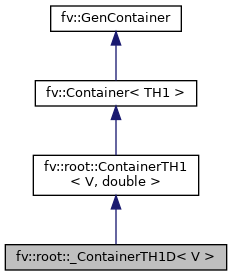
\includegraphics[width=246pt]{classfv_1_1root_1_1__ContainerTH1D__inherit__graph}
\end{center}
\end{figure}


Collaboration diagram for fv\+:\+:root\+:\+:\+\_\+\+Container\+T\+H1D$<$ V $>$\+:
\nopagebreak
\begin{figure}[H]
\begin{center}
\leavevmode
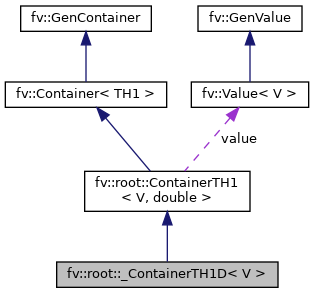
\includegraphics[width=308pt]{classfv_1_1root_1_1__ContainerTH1D__coll__graph}
\end{center}
\end{figure}
\subsection*{Private Member Functions}
\begin{DoxyCompactItemize}
\item 
\hypertarget{classfv_1_1root_1_1__ContainerTH1D_aaa0ad5b59d5b8d3ecf71d8b2c8be1375}{}\label{classfv_1_1root_1_1__ContainerTH1D_aaa0ad5b59d5b8d3ecf71d8b2c8be1375} 
void {\bfseries init\+\_\+\+T\+H1} ()
\end{DoxyCompactItemize}
\subsection*{Additional Inherited Members}


The documentation for this class was generated from the following file\+:\begin{DoxyCompactItemize}
\item 
/home/caleb/\+Sources/\+T\+T\+T\+T/filval\+\_\+root/container.\+hpp\end{DoxyCompactItemize}

\hypertarget{classfv_1_1root_1_1__ContainerTH1F}{}\section{fv\+:\+:root\+:\+:\+\_\+\+Container\+T\+H1F$<$ V $>$ Class Template Reference}
\label{classfv_1_1root_1_1__ContainerTH1F}\index{fv\+::root\+::\+\_\+\+Container\+T\+H1\+F$<$ V $>$@{fv\+::root\+::\+\_\+\+Container\+T\+H1\+F$<$ V $>$}}


Inheritance diagram for fv\+:\+:root\+:\+:\+\_\+\+Container\+T\+H1F$<$ V $>$\+:
\nopagebreak
\begin{figure}[H]
\begin{center}
\leavevmode
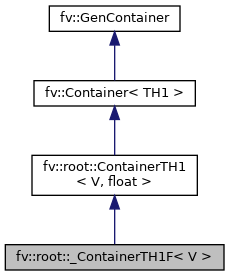
\includegraphics[width=244pt]{classfv_1_1root_1_1__ContainerTH1F__inherit__graph}
\end{center}
\end{figure}


Collaboration diagram for fv\+:\+:root\+:\+:\+\_\+\+Container\+T\+H1F$<$ V $>$\+:
\nopagebreak
\begin{figure}[H]
\begin{center}
\leavevmode
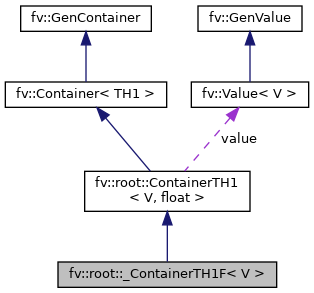
\includegraphics[width=308pt]{classfv_1_1root_1_1__ContainerTH1F__coll__graph}
\end{center}
\end{figure}
\subsection*{Private Member Functions}
\begin{DoxyCompactItemize}
\item 
\hypertarget{classfv_1_1root_1_1__ContainerTH1F_aeb6c270b6ac75c8f39cd89771a9597ee}{}\label{classfv_1_1root_1_1__ContainerTH1F_aeb6c270b6ac75c8f39cd89771a9597ee} 
void {\bfseries init\+\_\+\+T\+H1} ()
\end{DoxyCompactItemize}
\subsection*{Additional Inherited Members}


The documentation for this class was generated from the following file\+:\begin{DoxyCompactItemize}
\item 
/home/caleb/\+Sources/\+T\+T\+T\+T/filval\+\_\+root/container.\+hpp\end{DoxyCompactItemize}

\hypertarget{classfv_1_1root_1_1__ContainerTH1I}{}\section{fv\+:\+:root\+:\+:\+\_\+\+Container\+T\+H1I$<$ V $>$ Class Template Reference}
\label{classfv_1_1root_1_1__ContainerTH1I}\index{fv\+::root\+::\+\_\+\+Container\+T\+H1\+I$<$ V $>$@{fv\+::root\+::\+\_\+\+Container\+T\+H1\+I$<$ V $>$}}


Inheritance diagram for fv\+:\+:root\+:\+:\+\_\+\+Container\+T\+H1I$<$ V $>$\+:
\nopagebreak
\begin{figure}[H]
\begin{center}
\leavevmode
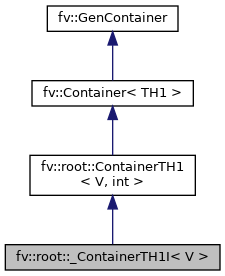
\includegraphics[width=241pt]{classfv_1_1root_1_1__ContainerTH1I__inherit__graph}
\end{center}
\end{figure}


Collaboration diagram for fv\+:\+:root\+:\+:\+\_\+\+Container\+T\+H1I$<$ V $>$\+:
\nopagebreak
\begin{figure}[H]
\begin{center}
\leavevmode
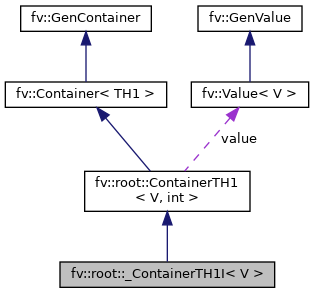
\includegraphics[width=308pt]{classfv_1_1root_1_1__ContainerTH1I__coll__graph}
\end{center}
\end{figure}
\subsection*{Private Member Functions}
\begin{DoxyCompactItemize}
\item 
\hypertarget{classfv_1_1root_1_1__ContainerTH1I_af25ca6034457d40efe3e513ba4ed6333}{}\label{classfv_1_1root_1_1__ContainerTH1I_af25ca6034457d40efe3e513ba4ed6333} 
void {\bfseries init\+\_\+\+T\+H1} ()
\end{DoxyCompactItemize}
\subsection*{Additional Inherited Members}


The documentation for this class was generated from the following file\+:\begin{DoxyCompactItemize}
\item 
/home/caleb/\+Sources/\+T\+T\+T\+T/filval\+\_\+root/container.\+hpp\end{DoxyCompactItemize}

\hypertarget{classfv_1_1root_1_1__ContainerTH2D}{}\section{fv\+:\+:root\+:\+:\+\_\+\+Container\+T\+H2D$<$ V $>$ Class Template Reference}
\label{classfv_1_1root_1_1__ContainerTH2D}\index{fv\+::root\+::\+\_\+\+Container\+T\+H2\+D$<$ V $>$@{fv\+::root\+::\+\_\+\+Container\+T\+H2\+D$<$ V $>$}}


Inheritance diagram for fv\+:\+:root\+:\+:\+\_\+\+Container\+T\+H2D$<$ V $>$\+:
\nopagebreak
\begin{figure}[H]
\begin{center}
\leavevmode
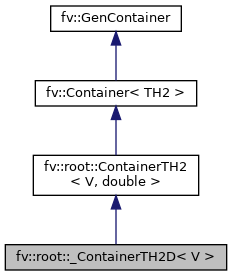
\includegraphics[width=246pt]{classfv_1_1root_1_1__ContainerTH2D__inherit__graph}
\end{center}
\end{figure}


Collaboration diagram for fv\+:\+:root\+:\+:\+\_\+\+Container\+T\+H2D$<$ V $>$\+:
\nopagebreak
\begin{figure}[H]
\begin{center}
\leavevmode
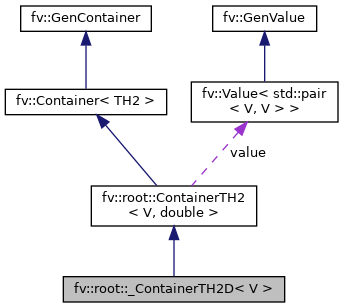
\includegraphics[width=330pt]{classfv_1_1root_1_1__ContainerTH2D__coll__graph}
\end{center}
\end{figure}
\subsection*{Private Member Functions}
\begin{DoxyCompactItemize}
\item 
\hypertarget{classfv_1_1root_1_1__ContainerTH2D_a2d3395e53c89cce573de1e62dcf344bb}{}\label{classfv_1_1root_1_1__ContainerTH2D_a2d3395e53c89cce573de1e62dcf344bb} 
void {\bfseries init\+\_\+\+T\+H2} ()
\end{DoxyCompactItemize}
\subsection*{Additional Inherited Members}


The documentation for this class was generated from the following file\+:\begin{DoxyCompactItemize}
\item 
/home/caleb/\+Sources/\+T\+T\+T\+T/filval\+\_\+root/container.\+hpp\end{DoxyCompactItemize}

\hypertarget{classfv_1_1root_1_1__ContainerTH2F}{}\section{fv\+:\+:root\+:\+:\+\_\+\+Container\+T\+H2F$<$ V $>$ Class Template Reference}
\label{classfv_1_1root_1_1__ContainerTH2F}\index{fv\+::root\+::\+\_\+\+Container\+T\+H2\+F$<$ V $>$@{fv\+::root\+::\+\_\+\+Container\+T\+H2\+F$<$ V $>$}}


Inheritance diagram for fv\+:\+:root\+:\+:\+\_\+\+Container\+T\+H2F$<$ V $>$\+:
\nopagebreak
\begin{figure}[H]
\begin{center}
\leavevmode
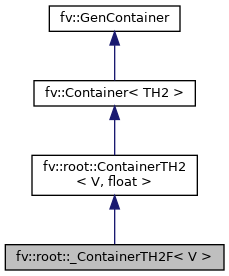
\includegraphics[width=244pt]{classfv_1_1root_1_1__ContainerTH2F__inherit__graph}
\end{center}
\end{figure}


Collaboration diagram for fv\+:\+:root\+:\+:\+\_\+\+Container\+T\+H2F$<$ V $>$\+:
\nopagebreak
\begin{figure}[H]
\begin{center}
\leavevmode
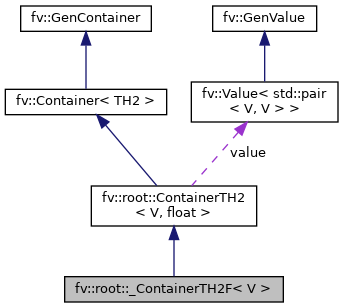
\includegraphics[width=330pt]{classfv_1_1root_1_1__ContainerTH2F__coll__graph}
\end{center}
\end{figure}
\subsection*{Private Member Functions}
\begin{DoxyCompactItemize}
\item 
\hypertarget{classfv_1_1root_1_1__ContainerTH2F_a041722b5c33266f78b1d75a2b2bf9579}{}\label{classfv_1_1root_1_1__ContainerTH2F_a041722b5c33266f78b1d75a2b2bf9579} 
void {\bfseries init\+\_\+\+T\+H2} ()
\end{DoxyCompactItemize}
\subsection*{Additional Inherited Members}


The documentation for this class was generated from the following file\+:\begin{DoxyCompactItemize}
\item 
/home/caleb/\+Sources/\+T\+T\+T\+T/filval\+\_\+root/container.\+hpp\end{DoxyCompactItemize}

\hypertarget{classfv_1_1root_1_1__ContainerTH2I}{}\section{fv\+:\+:root\+:\+:\+\_\+\+Container\+T\+H2I$<$ V $>$ Class Template Reference}
\label{classfv_1_1root_1_1__ContainerTH2I}\index{fv\+::root\+::\+\_\+\+Container\+T\+H2\+I$<$ V $>$@{fv\+::root\+::\+\_\+\+Container\+T\+H2\+I$<$ V $>$}}


Inheritance diagram for fv\+:\+:root\+:\+:\+\_\+\+Container\+T\+H2I$<$ V $>$\+:
\nopagebreak
\begin{figure}[H]
\begin{center}
\leavevmode
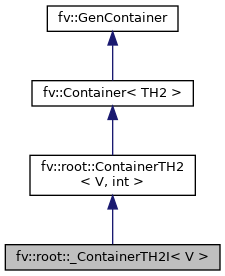
\includegraphics[width=241pt]{classfv_1_1root_1_1__ContainerTH2I__inherit__graph}
\end{center}
\end{figure}


Collaboration diagram for fv\+:\+:root\+:\+:\+\_\+\+Container\+T\+H2I$<$ V $>$\+:
\nopagebreak
\begin{figure}[H]
\begin{center}
\leavevmode
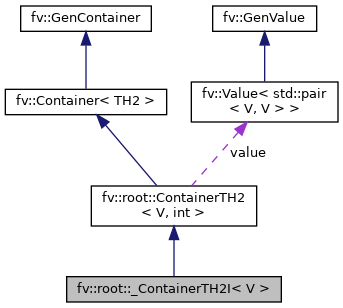
\includegraphics[width=330pt]{classfv_1_1root_1_1__ContainerTH2I__coll__graph}
\end{center}
\end{figure}
\subsection*{Private Member Functions}
\begin{DoxyCompactItemize}
\item 
\hypertarget{classfv_1_1root_1_1__ContainerTH2I_ade6b296e58561d8d255b2ad92f16a895}{}\label{classfv_1_1root_1_1__ContainerTH2I_ade6b296e58561d8d255b2ad92f16a895} 
void {\bfseries init\+\_\+\+T\+H2} ()
\end{DoxyCompactItemize}
\subsection*{Additional Inherited Members}


The documentation for this class was generated from the following file\+:\begin{DoxyCompactItemize}
\item 
/home/caleb/\+Sources/\+T\+T\+T\+T/filval\+\_\+root/container.\+hpp\end{DoxyCompactItemize}

\hypertarget{classfv_1_1util_1_1ArgParser}{}\section{fv\+:\+:util\+:\+:Arg\+Parser Class Reference}
\label{classfv_1_1util_1_1ArgParser}\index{fv\+::util\+::\+Arg\+Parser@{fv\+::util\+::\+Arg\+Parser}}
\subsection*{Public Member Functions}
\begin{DoxyCompactItemize}
\item 
\hypertarget{classfv_1_1util_1_1ArgParser_a4b712cf16ae946cd1c651e4275f1c39b}{}\label{classfv_1_1util_1_1ArgParser_a4b712cf16ae946cd1c651e4275f1c39b} 
{\bfseries Arg\+Parser} (int \&argc, char $\ast$$\ast$argv)
\item 
const std\+::string \& \hyperlink{classfv_1_1util_1_1ArgParser_aaeb266ab0e49cfee9691c8ad578a7688}{get\+Cmd\+Option} (const std\+::string \&option) const
\item 
bool \hyperlink{classfv_1_1util_1_1ArgParser_a4a1b9f8a41c5a6793a7b8f4ad82fc99c}{cmd\+Option\+Exists} (const std\+::string \&option) const
\end{DoxyCompactItemize}
\subsection*{Private Attributes}
\begin{DoxyCompactItemize}
\item 
\hypertarget{classfv_1_1util_1_1ArgParser_ac36e685804472836ec1e698937275242}{}\label{classfv_1_1util_1_1ArgParser_ac36e685804472836ec1e698937275242} 
std\+::vector$<$ std\+::string $>$ {\bfseries tokens}
\item 
\hypertarget{classfv_1_1util_1_1ArgParser_a3924e22ef57f754eb6f9c03a36952b80}{}\label{classfv_1_1util_1_1ArgParser_a3924e22ef57f754eb6f9c03a36952b80} 
std\+::string {\bfseries empty\+\_\+string}
\end{DoxyCompactItemize}


\subsection{Member Function Documentation}
\hypertarget{classfv_1_1util_1_1ArgParser_a4a1b9f8a41c5a6793a7b8f4ad82fc99c}{}\label{classfv_1_1util_1_1ArgParser_a4a1b9f8a41c5a6793a7b8f4ad82fc99c} 
\index{fv\+::util\+::\+Arg\+Parser@{fv\+::util\+::\+Arg\+Parser}!cmd\+Option\+Exists@{cmd\+Option\+Exists}}
\index{cmd\+Option\+Exists@{cmd\+Option\+Exists}!fv\+::util\+::\+Arg\+Parser@{fv\+::util\+::\+Arg\+Parser}}
\subsubsection{\texorpdfstring{cmd\+Option\+Exists()}{cmdOptionExists()}}
{\footnotesize\ttfamily bool fv\+::util\+::\+Arg\+Parser\+::cmd\+Option\+Exists (\begin{DoxyParamCaption}\item[{const std\+::string \&}]{option }\end{DoxyParamCaption}) const\hspace{0.3cm}{\ttfamily [inline]}}

\begin{DoxyAuthor}{Author}
iain 
\end{DoxyAuthor}
\hypertarget{classfv_1_1util_1_1ArgParser_aaeb266ab0e49cfee9691c8ad578a7688}{}\label{classfv_1_1util_1_1ArgParser_aaeb266ab0e49cfee9691c8ad578a7688} 
\index{fv\+::util\+::\+Arg\+Parser@{fv\+::util\+::\+Arg\+Parser}!get\+Cmd\+Option@{get\+Cmd\+Option}}
\index{get\+Cmd\+Option@{get\+Cmd\+Option}!fv\+::util\+::\+Arg\+Parser@{fv\+::util\+::\+Arg\+Parser}}
\subsubsection{\texorpdfstring{get\+Cmd\+Option()}{getCmdOption()}}
{\footnotesize\ttfamily const std\+::string\& fv\+::util\+::\+Arg\+Parser\+::get\+Cmd\+Option (\begin{DoxyParamCaption}\item[{const std\+::string \&}]{option }\end{DoxyParamCaption}) const\hspace{0.3cm}{\ttfamily [inline]}}

\begin{DoxyAuthor}{Author}
iain 
\end{DoxyAuthor}


The documentation for this class was generated from the following file\+:\begin{DoxyCompactItemize}
\item 
/home/caleb/\+Sources/\+T\+T\+T\+T/filval/\hyperlink{argparse_8hpp}{argparse.\+hpp}\end{DoxyCompactItemize}

\hypertarget{classfv_1_1BoundValue}{}\section{fv\+:\+:Bound\+Value$<$ T $>$ Class Template Reference}
\label{classfv_1_1BoundValue}\index{fv\+::\+Bound\+Value$<$ T $>$@{fv\+::\+Bound\+Value$<$ T $>$}}


A generic value owning only a function object.  




{\ttfamily \#include $<$value.\+hpp$>$}



Inheritance diagram for fv\+:\+:Bound\+Value$<$ T $>$\+:
\nopagebreak
\begin{figure}[H]
\begin{center}
\leavevmode
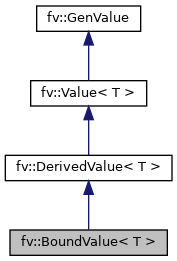
\includegraphics[width=205pt]{classfv_1_1BoundValue__inherit__graph}
\end{center}
\end{figure}


Collaboration diagram for fv\+:\+:Bound\+Value$<$ T $>$\+:
\nopagebreak
\begin{figure}[H]
\begin{center}
\leavevmode
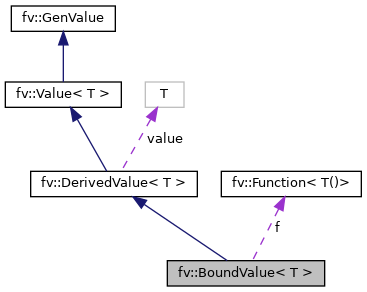
\includegraphics[width=347pt]{classfv_1_1BoundValue__coll__graph}
\end{center}
\end{figure}
\subsection*{Public Member Functions}
\begin{DoxyCompactItemize}
\item 
\hypertarget{classfv_1_1BoundValue_aa5157e0e9ba817cdeaef72f643ba8a79}{}\label{classfv_1_1BoundValue_aa5157e0e9ba817cdeaef72f643ba8a79} 
{\bfseries Bound\+Value} (\hyperlink{classfv_1_1Function}{Function}$<$ T()$>$ \&f, const std\+::string alias=\char`\"{}\char`\"{})
\end{DoxyCompactItemize}
\subsection*{Protected Member Functions}
\begin{DoxyCompactItemize}
\item 
void \hyperlink{classfv_1_1BoundValue_a51ba914f1eac694af4264d62785282a1}{update\+\_\+value} ()
\begin{DoxyCompactList}\small\item\em Updates the internal value. \end{DoxyCompactList}\end{DoxyCompactItemize}
\subsection*{Protected Attributes}
\begin{DoxyCompactItemize}
\item 
\hypertarget{classfv_1_1BoundValue_a09946c7cd867603db1b66d64a6d43e69}{}\label{classfv_1_1BoundValue_a09946c7cd867603db1b66d64a6d43e69} 
\hyperlink{classfv_1_1Function}{Function}$<$ T()$>$ \& {\bfseries f}
\end{DoxyCompactItemize}
\subsection*{Additional Inherited Members}


\subsection{Detailed Description}
\subsubsection*{template$<$typename T$>$\newline
class fv\+::\+Bound\+Value$<$ T $>$}

A generic value owning only a function object. 

All necessary values upon which this value depends must be bound to the function object. 

\subsection{Member Function Documentation}
\hypertarget{classfv_1_1BoundValue_a51ba914f1eac694af4264d62785282a1}{}\label{classfv_1_1BoundValue_a51ba914f1eac694af4264d62785282a1} 
\index{fv\+::\+Bound\+Value@{fv\+::\+Bound\+Value}!update\+\_\+value@{update\+\_\+value}}
\index{update\+\_\+value@{update\+\_\+value}!fv\+::\+Bound\+Value@{fv\+::\+Bound\+Value}}
\subsubsection{\texorpdfstring{update\+\_\+value()}{update\_value()}}
{\footnotesize\ttfamily template$<$typename T $>$ \\
void \hyperlink{classfv_1_1BoundValue}{fv\+::\+Bound\+Value}$<$ T $>$\+::update\+\_\+value (\begin{DoxyParamCaption}{ }\end{DoxyParamCaption})\hspace{0.3cm}{\ttfamily [inline]}, {\ttfamily [protected]}, {\ttfamily [virtual]}}



Updates the internal value. 

This function should be overridden by any child class to do the actual work of updating value based on whatever rules the class chooses. Normally, this consists of geting the values from some associated \hyperlink{classfv_1_1Value}{Value} objects, doing some calculation on them, and storing the result in value. 

Implements \hyperlink{classfv_1_1DerivedValue_ae59e80a98eb74b95d8961bfe12ee5ec2}{fv\+::\+Derived\+Value$<$ T $>$}.



The documentation for this class was generated from the following file\+:\begin{DoxyCompactItemize}
\item 
/home/caleb/\+Sources/\+T\+T\+T\+T/filval/\hyperlink{value_8hpp}{value.\+hpp}\end{DoxyCompactItemize}

\hypertarget{classfv_1_1ConstantValue}{}\section{fv\+:\+:Constant\+Value$<$ T $>$ Class Template Reference}
\label{classfv_1_1ConstantValue}\index{fv\+::\+Constant\+Value$<$ T $>$@{fv\+::\+Constant\+Value$<$ T $>$}}


A \hyperlink{classfv_1_1Value}{Value} which always returns the same value, supplied in the constructor.  




{\ttfamily \#include $<$value.\+hpp$>$}



Inheritance diagram for fv\+:\+:Constant\+Value$<$ T $>$\+:
\nopagebreak
\begin{figure}[H]
\begin{center}
\leavevmode
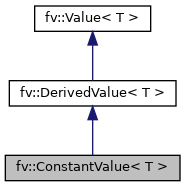
\includegraphics[width=211pt]{classfv_1_1ConstantValue__inherit__graph}
\end{center}
\end{figure}


Collaboration diagram for fv\+:\+:Constant\+Value$<$ T $>$\+:
\nopagebreak
\begin{figure}[H]
\begin{center}
\leavevmode
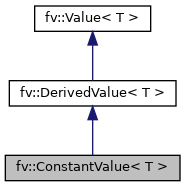
\includegraphics[width=283pt]{classfv_1_1ConstantValue__coll__graph}
\end{center}
\end{figure}
\subsection*{Public Member Functions}
\begin{DoxyCompactItemize}
\item 
\hypertarget{classfv_1_1ConstantValue_a82512bd0a0505bcf69816fa8b3305c29}{}\label{classfv_1_1ConstantValue_a82512bd0a0505bcf69816fa8b3305c29} 
{\bfseries Constant\+Value} (const std\+::string \&\hyperlink{classfv_1_1GenValue_a610f89ee441eaad4c9e78f74d6bde93b}{name}, T const\+\_\+value, const std\+::string alias=\char`\"{}\char`\"{})
\end{DoxyCompactItemize}
\subsection*{Protected Member Functions}
\begin{DoxyCompactItemize}
\item 
void \hyperlink{classfv_1_1ConstantValue_a6581e7fb69c082c07c9714138063b320}{update\+\_\+value} ()
\begin{DoxyCompactList}\small\item\em Updates the internal value. \end{DoxyCompactList}\end{DoxyCompactItemize}
\subsection*{Protected Attributes}
\begin{DoxyCompactItemize}
\item 
\hypertarget{classfv_1_1ConstantValue_a7bd409365b0f9a271a865d7d7abf1648}{}\label{classfv_1_1ConstantValue_a7bd409365b0f9a271a865d7d7abf1648} 
T {\bfseries const\+\_\+value}
\end{DoxyCompactItemize}
\subsection*{Additional Inherited Members}


\subsection{Detailed Description}
\subsubsection*{template$<$typename T$>$\newline
class fv\+::\+Constant\+Value$<$ T $>$}

A \hyperlink{classfv_1_1Value}{Value} which always returns the same value, supplied in the constructor. 

\subsection{Member Function Documentation}
\hypertarget{classfv_1_1ConstantValue_a6581e7fb69c082c07c9714138063b320}{}\label{classfv_1_1ConstantValue_a6581e7fb69c082c07c9714138063b320} 
\index{fv\+::\+Constant\+Value@{fv\+::\+Constant\+Value}!update\+\_\+value@{update\+\_\+value}}
\index{update\+\_\+value@{update\+\_\+value}!fv\+::\+Constant\+Value@{fv\+::\+Constant\+Value}}
\subsubsection{\texorpdfstring{update\+\_\+value()}{update\_value()}}
{\footnotesize\ttfamily template$<$typename T $>$ \\
void \hyperlink{classfv_1_1ConstantValue}{fv\+::\+Constant\+Value}$<$ T $>$\+::update\+\_\+value (\begin{DoxyParamCaption}{ }\end{DoxyParamCaption})\hspace{0.3cm}{\ttfamily [inline]}, {\ttfamily [protected]}, {\ttfamily [virtual]}}



Updates the internal value. 

This function should be overridden by any child class to do the actual work of updating value based on whatever rules the class chooses. Normally, this consists of geting the values from some associated \hyperlink{classfv_1_1Value}{Value} objects, doing some calculation on them, and storing the result in value. 

Implements \hyperlink{classfv_1_1DerivedValue_ae59e80a98eb74b95d8961bfe12ee5ec2}{fv\+::\+Derived\+Value$<$ T $>$}.



The documentation for this class was generated from the following file\+:\begin{DoxyCompactItemize}
\item 
/home/caleb/\+Sources/\+T\+T\+T\+T/filval/\hyperlink{value_8hpp}{value.\+hpp}\end{DoxyCompactItemize}

\hypertarget{classfv_1_1Container}{}\section{fv\+:\+:Container$<$ H $>$ Class Template Reference}
\label{classfv_1_1Container}\index{fv\+::\+Container$<$ H $>$@{fv\+::\+Container$<$ H $>$}}


Inheritance diagram for fv\+:\+:Container$<$ H $>$\+:
\nopagebreak
\begin{figure}[H]
\begin{center}
\leavevmode
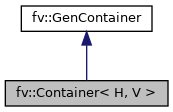
\includegraphics[width=189pt]{classfv_1_1Container__inherit__graph}
\end{center}
\end{figure}


Collaboration diagram for fv\+:\+:Container$<$ H $>$\+:
\nopagebreak
\begin{figure}[H]
\begin{center}
\leavevmode
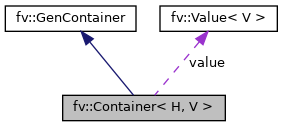
\includegraphics[width=241pt]{classfv_1_1Container__coll__graph}
\end{center}
\end{figure}
\subsection*{Public Member Functions}
\begin{DoxyCompactItemize}
\item 
\hypertarget{classfv_1_1Container_af182df68521c2b1f61f5b6c330508255}{}\label{classfv_1_1Container_af182df68521c2b1f61f5b6c330508255} 
{\bfseries Container} (const std\+::string \&name, H $\ast$container)
\item 
\hypertarget{classfv_1_1Container_af3caa2b464b5984690392f8b0e9f9c78}{}\label{classfv_1_1Container_af3caa2b464b5984690392f8b0e9f9c78} 
virtual H $\ast$ {\bfseries get\+\_\+container} ()
\end{DoxyCompactItemize}
\subsection*{Protected Attributes}
\begin{DoxyCompactItemize}
\item 
\hypertarget{classfv_1_1Container_aa5e74e62f69e756cad950fdc94e9a8c0}{}\label{classfv_1_1Container_aa5e74e62f69e756cad950fdc94e9a8c0} 
H $\ast$ {\bfseries container}
\end{DoxyCompactItemize}
\subsection*{Additional Inherited Members}


The documentation for this class was generated from the following file\+:\begin{DoxyCompactItemize}
\item 
/home/caleb/\+Sources/\+T\+T\+T\+T/filval/container.\+hpp\end{DoxyCompactItemize}

\hypertarget{classfv_1_1ContainerMean}{}\section{fv\+:\+:Container\+Mean$<$ T $>$ Class Template Reference}
\label{classfv_1_1ContainerMean}\index{fv\+::\+Container\+Mean$<$ T $>$@{fv\+::\+Container\+Mean$<$ T $>$}}


Inheritance diagram for fv\+:\+:Container\+Mean$<$ T $>$\+:
\nopagebreak
\begin{figure}[H]
\begin{center}
\leavevmode
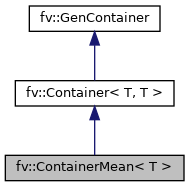
\includegraphics[width=214pt]{classfv_1_1ContainerMean__inherit__graph}
\end{center}
\end{figure}


Collaboration diagram for fv\+:\+:Container\+Mean$<$ T $>$\+:
\nopagebreak
\begin{figure}[H]
\begin{center}
\leavevmode
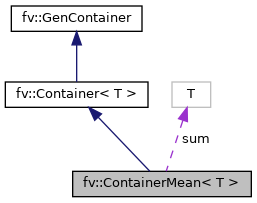
\includegraphics[width=265pt]{classfv_1_1ContainerMean__coll__graph}
\end{center}
\end{figure}
\subsection*{Public Member Functions}
\begin{DoxyCompactItemize}
\item 
\hypertarget{classfv_1_1ContainerMean_a6a577d9ee5d9aeff0918d192974262e1}{}\label{classfv_1_1ContainerMean_a6a577d9ee5d9aeff0918d192974262e1} 
{\bfseries Container\+Mean} (const std\+::string \&name, \hyperlink{classfv_1_1Value}{Value}$<$ T $>$ $\ast$value)
\item 
\hypertarget{classfv_1_1ContainerMean_ad02d976b076e3fb6ad3bb15eb35406d4}{}\label{classfv_1_1ContainerMean_ad02d976b076e3fb6ad3bb15eb35406d4} 
T $\ast$ {\bfseries get\+\_\+container} ()
\item 
\hypertarget{classfv_1_1ContainerMean_a9fa3d582ae665ea4f5ee1c7215fe0ff0}{}\label{classfv_1_1ContainerMean_a9fa3d582ae665ea4f5ee1c7215fe0ff0} 
void {\bfseries save\+\_\+as} (const std\+::string \&fname)
\item 
\hypertarget{classfv_1_1ContainerMean_ab917d198ce468125b06c71dbe77e5c59}{}\label{classfv_1_1ContainerMean_ab917d198ce468125b06c71dbe77e5c59} 
virtual void {\bfseries save} ()
\end{DoxyCompactItemize}
\subsection*{Private Member Functions}
\begin{DoxyCompactItemize}
\item 
\hypertarget{classfv_1_1ContainerMean_a5f6d834f6490729852fb807feb775a75}{}\label{classfv_1_1ContainerMean_a5f6d834f6490729852fb807feb775a75} 
void {\bfseries \+\_\+fill} ()
\end{DoxyCompactItemize}
\subsection*{Private Attributes}
\begin{DoxyCompactItemize}
\item 
\hypertarget{classfv_1_1ContainerMean_aa772cde78fd0971d1ebba909aff491c1}{}\label{classfv_1_1ContainerMean_aa772cde78fd0971d1ebba909aff491c1} 
\hyperlink{classfv_1_1Value}{Value}$<$ T $>$ $\ast$ {\bfseries value}
\item 
\hypertarget{classfv_1_1ContainerMean_a39cdef23a358ab46173eaa588e59ce49}{}\label{classfv_1_1ContainerMean_a39cdef23a358ab46173eaa588e59ce49} 
int {\bfseries count}
\item 
\hypertarget{classfv_1_1ContainerMean_ac85f2f56241ebf5099784250288c585b}{}\label{classfv_1_1ContainerMean_ac85f2f56241ebf5099784250288c585b} 
T {\bfseries sum}
\end{DoxyCompactItemize}
\subsection*{Additional Inherited Members}


The documentation for this class was generated from the following file\+:\begin{DoxyCompactItemize}
\item 
/home/caleb/\+Sources/\+T\+T\+T\+T/filval/container.\+hpp\end{DoxyCompactItemize}

\hypertarget{classfv_1_1root_1_1ContainerTGraph}{}\section{fv\+:\+:root\+:\+:Container\+T\+Graph Class Reference}
\label{classfv_1_1root_1_1ContainerTGraph}\index{fv\+::root\+::\+Container\+T\+Graph@{fv\+::root\+::\+Container\+T\+Graph}}


Inheritance diagram for fv\+:\+:root\+:\+:Container\+T\+Graph\+:
\nopagebreak
\begin{figure}[H]
\begin{center}
\leavevmode
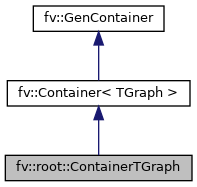
\includegraphics[width=220pt]{classfv_1_1root_1_1ContainerTGraph__inherit__graph}
\end{center}
\end{figure}


Collaboration diagram for fv\+:\+:root\+:\+:Container\+T\+Graph\+:
\nopagebreak
\begin{figure}[H]
\begin{center}
\leavevmode
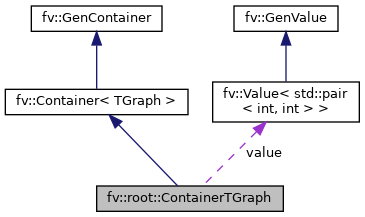
\includegraphics[width=346pt]{classfv_1_1root_1_1ContainerTGraph__coll__graph}
\end{center}
\end{figure}
\subsection*{Public Member Functions}
\begin{DoxyCompactItemize}
\item 
\hypertarget{classfv_1_1root_1_1ContainerTGraph_a6ce03e340c2e2f5922ba6a9799eee7ef}{}\label{classfv_1_1root_1_1ContainerTGraph_a6ce03e340c2e2f5922ba6a9799eee7ef} 
{\bfseries Container\+T\+Graph} (const std\+::string \&name, \hyperlink{classfv_1_1GenValue}{Gen\+Value} $\ast$value)
\item 
\hypertarget{classfv_1_1root_1_1ContainerTGraph_a0d34a4afcd209b05353dce701e416b87}{}\label{classfv_1_1root_1_1ContainerTGraph_a0d34a4afcd209b05353dce701e416b87} 
T\+Graph $\ast$ {\bfseries get\+\_\+container} ()
\item 
\hypertarget{classfv_1_1root_1_1ContainerTGraph_a0269333d693b56b4e29c373cca6d64d8}{}\label{classfv_1_1root_1_1ContainerTGraph_a0269333d693b56b4e29c373cca6d64d8} 
void {\bfseries save\+\_\+as} (const std\+::string \&fname, const Save\+Option \&option=Save\+Option\+::\+P\+NG)
\end{DoxyCompactItemize}
\subsection*{Private Member Functions}
\begin{DoxyCompactItemize}
\item 
\hypertarget{classfv_1_1root_1_1ContainerTGraph_a7d0e25feb16f85c305fda6667554b6dc}{}\label{classfv_1_1root_1_1ContainerTGraph_a7d0e25feb16f85c305fda6667554b6dc} 
void {\bfseries \+\_\+fill} ()
\end{DoxyCompactItemize}
\subsection*{Private Attributes}
\begin{DoxyCompactItemize}
\item 
\hypertarget{classfv_1_1root_1_1ContainerTGraph_a5b58f77ca3c34042d4ca7d7bf91ccdb1}{}\label{classfv_1_1root_1_1ContainerTGraph_a5b58f77ca3c34042d4ca7d7bf91ccdb1} 
\hyperlink{classfv_1_1Value}{Value}$<$ std\+::pair$<$ int, int $>$ $>$ $\ast$ {\bfseries value}
\item 
\hypertarget{classfv_1_1root_1_1ContainerTGraph_ae518129625f7a8100f5800d418f05c2e}{}\label{classfv_1_1root_1_1ContainerTGraph_ae518129625f7a8100f5800d418f05c2e} 
std\+::vector$<$ int $>$ {\bfseries x\+\_\+data}
\item 
\hypertarget{classfv_1_1root_1_1ContainerTGraph_a7f971c3080be619b6fe83150caccfe68}{}\label{classfv_1_1root_1_1ContainerTGraph_a7f971c3080be619b6fe83150caccfe68} 
std\+::vector$<$ int $>$ {\bfseries y\+\_\+data}
\item 
\hypertarget{classfv_1_1root_1_1ContainerTGraph_aef25624d82dc794957ecfc13e853c165}{}\label{classfv_1_1root_1_1ContainerTGraph_aef25624d82dc794957ecfc13e853c165} 
bool {\bfseries data\+\_\+modified}
\end{DoxyCompactItemize}
\subsection*{Additional Inherited Members}


The documentation for this class was generated from the following file\+:\begin{DoxyCompactItemize}
\item 
/home/caleb/\+Sources/\+T\+T\+T\+T/filval\+\_\+root/container.\+hpp\end{DoxyCompactItemize}

\hypertarget{classfv_1_1root_1_1ContainerTH1}{}\section{fv\+:\+:root\+:\+:Container\+T\+H1$<$ V, D $>$ Class Template Reference}
\label{classfv_1_1root_1_1ContainerTH1}\index{fv\+::root\+::\+Container\+T\+H1$<$ V, D $>$@{fv\+::root\+::\+Container\+T\+H1$<$ V, D $>$}}


Inheritance diagram for fv\+:\+:root\+:\+:Container\+T\+H1$<$ V, D $>$\+:
\nopagebreak
\begin{figure}[H]
\begin{center}
\leavevmode
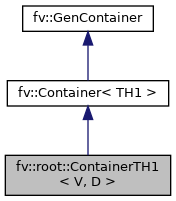
\includegraphics[width=204pt]{classfv_1_1root_1_1ContainerTH1__inherit__graph}
\end{center}
\end{figure}


Collaboration diagram for fv\+:\+:root\+:\+:Container\+T\+H1$<$ V, D $>$\+:
\nopagebreak
\begin{figure}[H]
\begin{center}
\leavevmode
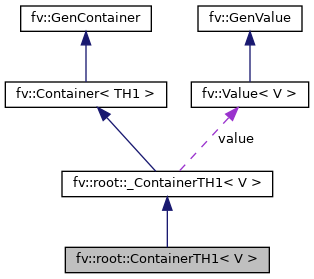
\includegraphics[width=350pt]{classfv_1_1root_1_1ContainerTH1__coll__graph}
\end{center}
\end{figure}
\subsection*{Public Member Functions}
\begin{DoxyCompactItemize}
\item 
\hypertarget{classfv_1_1root_1_1ContainerTH1_a5b2633b7ac0e398eb1fee32493af9787}{}\label{classfv_1_1root_1_1ContainerTH1_a5b2633b7ac0e398eb1fee32493af9787} 
{\bfseries Container\+T\+H1} (const std\+::string \&name, const std\+::string \&title, \hyperlink{classfv_1_1GenValue}{Gen\+Value} $\ast$value, int nbins, D low, D high)
\item 
\hypertarget{classfv_1_1root_1_1ContainerTH1_a552e1df4c424ab98206033b3ff8f6bd1}{}\label{classfv_1_1root_1_1ContainerTH1_a552e1df4c424ab98206033b3ff8f6bd1} 
void {\bfseries save\+\_\+as} (const std\+::string \&fname, const Save\+Option \&option=Save\+Option\+::\+P\+NG)
\end{DoxyCompactItemize}
\subsection*{Protected Member Functions}
\begin{DoxyCompactItemize}
\item 
\hypertarget{classfv_1_1root_1_1ContainerTH1_af9fe1115dc1e587974fa754b91656fba}{}\label{classfv_1_1root_1_1ContainerTH1_af9fe1115dc1e587974fa754b91656fba} 
virtual void {\bfseries init\+\_\+\+T\+H1} ()=0
\item 
\hypertarget{classfv_1_1root_1_1ContainerTH1_a459da5a66c6e582fe4cbe2b509247e20}{}\label{classfv_1_1root_1_1ContainerTH1_a459da5a66c6e582fe4cbe2b509247e20} 
virtual void {\bfseries \+\_\+do\+\_\+fill} (V \&val)=0
\end{DoxyCompactItemize}
\subsection*{Protected Attributes}
\begin{DoxyCompactItemize}
\item 
\hypertarget{classfv_1_1root_1_1ContainerTH1_a9778e00b2e0703499db8ff0ff07b11eb}{}\label{classfv_1_1root_1_1ContainerTH1_a9778e00b2e0703499db8ff0ff07b11eb} 
std\+::string {\bfseries title}
\item 
\hypertarget{classfv_1_1root_1_1ContainerTH1_abd1f59dcbfa3fdded4798f33eeb8449b}{}\label{classfv_1_1root_1_1ContainerTH1_abd1f59dcbfa3fdded4798f33eeb8449b} 
int {\bfseries nbins}
\item 
\hypertarget{classfv_1_1root_1_1ContainerTH1_a52ba4700aee1636a0ae9304dbecd4a29}{}\label{classfv_1_1root_1_1ContainerTH1_a52ba4700aee1636a0ae9304dbecd4a29} 
D {\bfseries low}
\item 
\hypertarget{classfv_1_1root_1_1ContainerTH1_afb62f146c619d79867275ba559c3df8e}{}\label{classfv_1_1root_1_1ContainerTH1_afb62f146c619d79867275ba559c3df8e} 
D {\bfseries high}
\item 
\hypertarget{classfv_1_1root_1_1ContainerTH1_a5d91fe71636d55f86f6e3104fc093787}{}\label{classfv_1_1root_1_1ContainerTH1_a5d91fe71636d55f86f6e3104fc093787} 
\hyperlink{classfv_1_1Value}{Value}$<$ V $>$ $\ast$ {\bfseries value}
\end{DoxyCompactItemize}
\subsection*{Private Member Functions}
\begin{DoxyCompactItemize}
\item 
\hypertarget{classfv_1_1root_1_1ContainerTH1_afd4218b3b43bba19cf5079439e7ce51f}{}\label{classfv_1_1root_1_1ContainerTH1_afd4218b3b43bba19cf5079439e7ce51f} 
void {\bfseries \+\_\+fill} ()
\end{DoxyCompactItemize}


The documentation for this class was generated from the following file\+:\begin{DoxyCompactItemize}
\item 
/home/caleb/\+Sources/\+T\+T\+T\+T/filval\+\_\+root/container.\+hpp\end{DoxyCompactItemize}

\hypertarget{classfv_1_1root_1_1ContainerTH1D}{}\section{fv\+:\+:root\+:\+:Container\+T\+H1D Class Reference}
\label{classfv_1_1root_1_1ContainerTH1D}\index{fv\+::root\+::\+Container\+T\+H1D@{fv\+::root\+::\+Container\+T\+H1D}}


Inheritance diagram for fv\+:\+:root\+:\+:Container\+T\+H1D\+:
\nopagebreak
\begin{figure}[H]
\begin{center}
\leavevmode
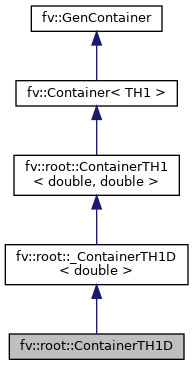
\includegraphics[width=217pt]{classfv_1_1root_1_1ContainerTH1D__inherit__graph}
\end{center}
\end{figure}


Collaboration diagram for fv\+:\+:root\+:\+:Container\+T\+H1D\+:
\nopagebreak
\begin{figure}[H]
\begin{center}
\leavevmode
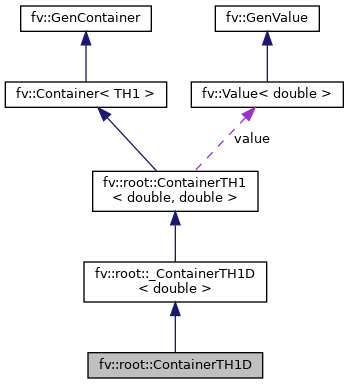
\includegraphics[width=334pt]{classfv_1_1root_1_1ContainerTH1D__coll__graph}
\end{center}
\end{figure}
\subsection*{Private Member Functions}
\begin{DoxyCompactItemize}
\item 
\hypertarget{classfv_1_1root_1_1ContainerTH1D_abdbef4ab1e5c567eb4ef2826df2f283e}{}\label{classfv_1_1root_1_1ContainerTH1D_abdbef4ab1e5c567eb4ef2826df2f283e} 
void {\bfseries \+\_\+do\+\_\+fill} (double \&val)
\end{DoxyCompactItemize}
\subsection*{Additional Inherited Members}


The documentation for this class was generated from the following file\+:\begin{DoxyCompactItemize}
\item 
/home/caleb/\+Sources/\+T\+T\+T\+T/filval\+\_\+root/container.\+hpp\end{DoxyCompactItemize}

\hypertarget{classfv_1_1root_1_1ContainerTH1DMany}{}\section{fv\+:\+:root\+:\+:Container\+T\+H1\+D\+Many Class Reference}
\label{classfv_1_1root_1_1ContainerTH1DMany}\index{fv\+::root\+::\+Container\+T\+H1\+D\+Many@{fv\+::root\+::\+Container\+T\+H1\+D\+Many}}


Inheritance diagram for fv\+:\+:root\+:\+:Container\+T\+H1\+D\+Many\+:
\nopagebreak
\begin{figure}[H]
\begin{center}
\leavevmode
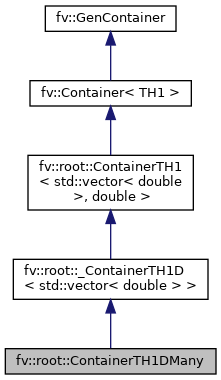
\includegraphics[width=238pt]{classfv_1_1root_1_1ContainerTH1DMany__inherit__graph}
\end{center}
\end{figure}


Collaboration diagram for fv\+:\+:root\+:\+:Container\+T\+H1\+D\+Many\+:
\nopagebreak
\begin{figure}[H]
\begin{center}
\leavevmode
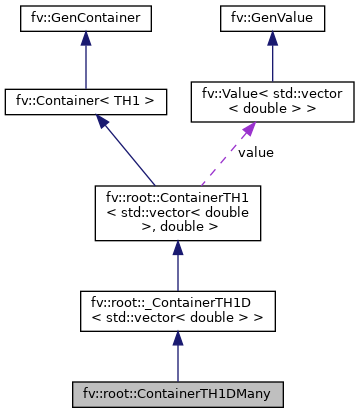
\includegraphics[width=342pt]{classfv_1_1root_1_1ContainerTH1DMany__coll__graph}
\end{center}
\end{figure}
\subsection*{Private Member Functions}
\begin{DoxyCompactItemize}
\item 
\hypertarget{classfv_1_1root_1_1ContainerTH1DMany_aa0b62d95327e836a79c50b1d637777e9}{}\label{classfv_1_1root_1_1ContainerTH1DMany_aa0b62d95327e836a79c50b1d637777e9} 
void {\bfseries \+\_\+do\+\_\+fill} (std\+::vector$<$ double $>$ \&val)
\end{DoxyCompactItemize}
\subsection*{Additional Inherited Members}


The documentation for this class was generated from the following file\+:\begin{DoxyCompactItemize}
\item 
/home/caleb/\+Sources/\+T\+T\+T\+T/filval\+\_\+root/container.\+hpp\end{DoxyCompactItemize}

\hypertarget{classfv_1_1root_1_1ContainerTH1F}{}\section{fv\+:\+:root\+:\+:Container\+T\+H1F Class Reference}
\label{classfv_1_1root_1_1ContainerTH1F}\index{fv\+::root\+::\+Container\+T\+H1F@{fv\+::root\+::\+Container\+T\+H1F}}


Inheritance diagram for fv\+:\+:root\+:\+:Container\+T\+H1F\+:
\nopagebreak
\begin{figure}[H]
\begin{center}
\leavevmode
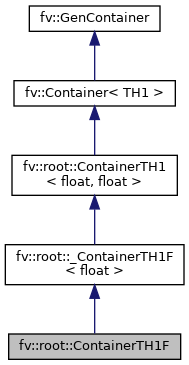
\includegraphics[width=214pt]{classfv_1_1root_1_1ContainerTH1F__inherit__graph}
\end{center}
\end{figure}


Collaboration diagram for fv\+:\+:root\+:\+:Container\+T\+H1F\+:
\nopagebreak
\begin{figure}[H]
\begin{center}
\leavevmode
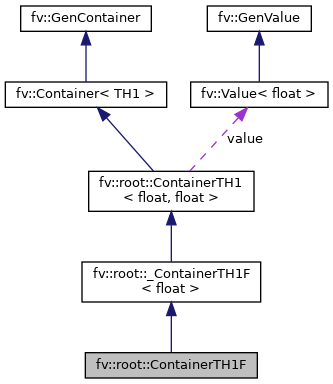
\includegraphics[width=322pt]{classfv_1_1root_1_1ContainerTH1F__coll__graph}
\end{center}
\end{figure}
\subsection*{Private Member Functions}
\begin{DoxyCompactItemize}
\item 
\hypertarget{classfv_1_1root_1_1ContainerTH1F_ae76e459ed2d830d22756064145f840c4}{}\label{classfv_1_1root_1_1ContainerTH1F_ae76e459ed2d830d22756064145f840c4} 
void {\bfseries \+\_\+do\+\_\+fill} (float \&val)
\end{DoxyCompactItemize}
\subsection*{Additional Inherited Members}


The documentation for this class was generated from the following file\+:\begin{DoxyCompactItemize}
\item 
/home/caleb/\+Sources/\+T\+T\+T\+T/filval\+\_\+root/container.\+hpp\end{DoxyCompactItemize}

\hypertarget{classfv_1_1root_1_1ContainerTH1FMany}{}\section{fv\+:\+:root\+:\+:Container\+T\+H1\+F\+Many Class Reference}
\label{classfv_1_1root_1_1ContainerTH1FMany}\index{fv\+::root\+::\+Container\+T\+H1\+F\+Many@{fv\+::root\+::\+Container\+T\+H1\+F\+Many}}


Inheritance diagram for fv\+:\+:root\+:\+:Container\+T\+H1\+F\+Many\+:
\nopagebreak
\begin{figure}[H]
\begin{center}
\leavevmode
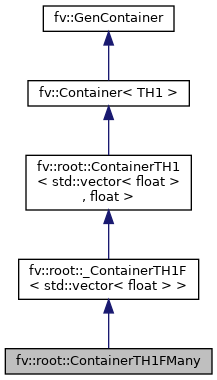
\includegraphics[width=235pt]{classfv_1_1root_1_1ContainerTH1FMany__inherit__graph}
\end{center}
\end{figure}


Collaboration diagram for fv\+:\+:root\+:\+:Container\+T\+H1\+F\+Many\+:
\nopagebreak
\begin{figure}[H]
\begin{center}
\leavevmode
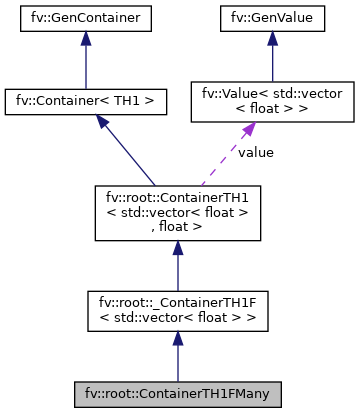
\includegraphics[width=342pt]{classfv_1_1root_1_1ContainerTH1FMany__coll__graph}
\end{center}
\end{figure}
\subsection*{Private Member Functions}
\begin{DoxyCompactItemize}
\item 
\hypertarget{classfv_1_1root_1_1ContainerTH1FMany_a326b73cef303ee804edff65c1da2d32c}{}\label{classfv_1_1root_1_1ContainerTH1FMany_a326b73cef303ee804edff65c1da2d32c} 
void {\bfseries \+\_\+do\+\_\+fill} (std\+::vector$<$ float $>$ \&val)
\end{DoxyCompactItemize}
\subsection*{Additional Inherited Members}


The documentation for this class was generated from the following file\+:\begin{DoxyCompactItemize}
\item 
/home/caleb/\+Sources/\+T\+T\+T\+T/filval\+\_\+root/container.\+hpp\end{DoxyCompactItemize}

\hypertarget{classfv_1_1root_1_1ContainerTH1I}{}\section{fv\+:\+:root\+:\+:Container\+T\+H1I Class Reference}
\label{classfv_1_1root_1_1ContainerTH1I}\index{fv\+::root\+::\+Container\+T\+H1I@{fv\+::root\+::\+Container\+T\+H1I}}


Inheritance diagram for fv\+:\+:root\+:\+:Container\+T\+H1I\+:
\nopagebreak
\begin{figure}[H]
\begin{center}
\leavevmode
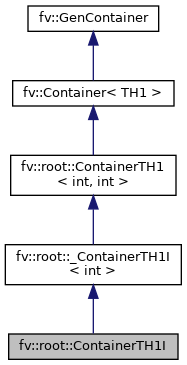
\includegraphics[width=212pt]{classfv_1_1root_1_1ContainerTH1I__inherit__graph}
\end{center}
\end{figure}


Collaboration diagram for fv\+:\+:root\+:\+:Container\+T\+H1I\+:
\nopagebreak
\begin{figure}[H]
\begin{center}
\leavevmode
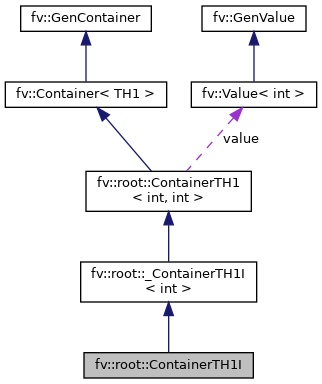
\includegraphics[width=314pt]{classfv_1_1root_1_1ContainerTH1I__coll__graph}
\end{center}
\end{figure}
\subsection*{Private Member Functions}
\begin{DoxyCompactItemize}
\item 
\hypertarget{classfv_1_1root_1_1ContainerTH1I_a33ca78d19d5e44f40580105cb0014e04}{}\label{classfv_1_1root_1_1ContainerTH1I_a33ca78d19d5e44f40580105cb0014e04} 
void {\bfseries \+\_\+do\+\_\+fill} (int \&val)
\end{DoxyCompactItemize}
\subsection*{Additional Inherited Members}


The documentation for this class was generated from the following file\+:\begin{DoxyCompactItemize}
\item 
/home/caleb/\+Sources/\+T\+T\+T\+T/filval\+\_\+root/container.\+hpp\end{DoxyCompactItemize}

\hypertarget{classfv_1_1root_1_1ContainerTH1IMany}{}\section{fv\+:\+:root\+:\+:Container\+T\+H1\+I\+Many Class Reference}
\label{classfv_1_1root_1_1ContainerTH1IMany}\index{fv\+::root\+::\+Container\+T\+H1\+I\+Many@{fv\+::root\+::\+Container\+T\+H1\+I\+Many}}


Inheritance diagram for fv\+:\+:root\+:\+:Container\+T\+H1\+I\+Many\+:
\nopagebreak
\begin{figure}[H]
\begin{center}
\leavevmode
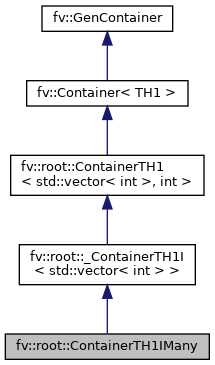
\includegraphics[width=233pt]{classfv_1_1root_1_1ContainerTH1IMany__inherit__graph}
\end{center}
\end{figure}


Collaboration diagram for fv\+:\+:root\+:\+:Container\+T\+H1\+I\+Many\+:
\nopagebreak
\begin{figure}[H]
\begin{center}
\leavevmode
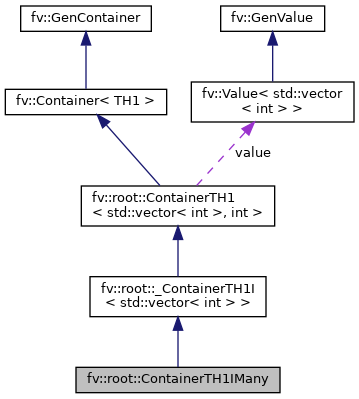
\includegraphics[width=342pt]{classfv_1_1root_1_1ContainerTH1IMany__coll__graph}
\end{center}
\end{figure}
\subsection*{Private Member Functions}
\begin{DoxyCompactItemize}
\item 
\hypertarget{classfv_1_1root_1_1ContainerTH1IMany_af04f55e12ac890d540f64f97852f153b}{}\label{classfv_1_1root_1_1ContainerTH1IMany_af04f55e12ac890d540f64f97852f153b} 
void {\bfseries \+\_\+do\+\_\+fill} (std\+::vector$<$ int $>$ \&val)
\end{DoxyCompactItemize}
\subsection*{Additional Inherited Members}


The documentation for this class was generated from the following file\+:\begin{DoxyCompactItemize}
\item 
/home/caleb/\+Sources/\+T\+T\+T\+T/filval\+\_\+root/container.\+hpp\end{DoxyCompactItemize}

\hypertarget{classfv_1_1root_1_1ContainerTH2}{}\section{fv\+:\+:root\+:\+:Container\+T\+H2$<$ V, D $>$ Class Template Reference}
\label{classfv_1_1root_1_1ContainerTH2}\index{fv\+::root\+::\+Container\+T\+H2$<$ V, D $>$@{fv\+::root\+::\+Container\+T\+H2$<$ V, D $>$}}


Inheritance diagram for fv\+:\+:root\+:\+:Container\+T\+H2$<$ V, D $>$\+:
\nopagebreak
\begin{figure}[H]
\begin{center}
\leavevmode
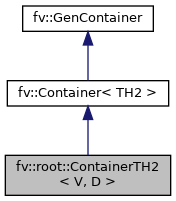
\includegraphics[width=204pt]{classfv_1_1root_1_1ContainerTH2__inherit__graph}
\end{center}
\end{figure}


Collaboration diagram for fv\+:\+:root\+:\+:Container\+T\+H2$<$ V, D $>$\+:
\nopagebreak
\begin{figure}[H]
\begin{center}
\leavevmode
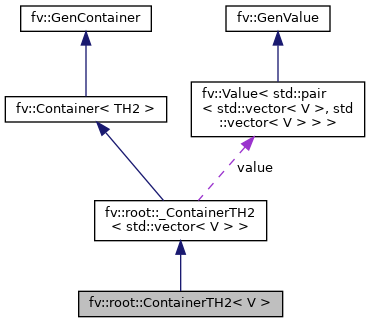
\includegraphics[width=350pt]{classfv_1_1root_1_1ContainerTH2__coll__graph}
\end{center}
\end{figure}
\subsection*{Public Member Functions}
\begin{DoxyCompactItemize}
\item 
\hypertarget{classfv_1_1root_1_1ContainerTH2_a2b0419d5acc2d1c0f5812105b0509ff0}{}\label{classfv_1_1root_1_1ContainerTH2_a2b0419d5acc2d1c0f5812105b0509ff0} 
{\bfseries Container\+T\+H2} (const std\+::string \&name, const std\+::string \&title, \hyperlink{classfv_1_1GenValue}{Gen\+Value} $\ast$value, int nbins\+\_\+x, D low\+\_\+x, D high\+\_\+x, int nbins\+\_\+y, D low\+\_\+y, D high\+\_\+y)
\item 
\hypertarget{classfv_1_1root_1_1ContainerTH2_ac22e15adea4f5338e2592fc0a239771d}{}\label{classfv_1_1root_1_1ContainerTH2_ac22e15adea4f5338e2592fc0a239771d} 
void {\bfseries save\+\_\+as} (const std\+::string \&fname, const Save\+Option \&option=Save\+Option\+::\+P\+NG)
\end{DoxyCompactItemize}
\subsection*{Protected Member Functions}
\begin{DoxyCompactItemize}
\item 
\hypertarget{classfv_1_1root_1_1ContainerTH2_af9056cafd1a764a54dfd17ca417ed0db}{}\label{classfv_1_1root_1_1ContainerTH2_af9056cafd1a764a54dfd17ca417ed0db} 
virtual void {\bfseries init\+\_\+\+T\+H2} ()=0
\item 
\hypertarget{classfv_1_1root_1_1ContainerTH2_a7a52f5fa3875d7f44645cc206902d9c2}{}\label{classfv_1_1root_1_1ContainerTH2_a7a52f5fa3875d7f44645cc206902d9c2} 
virtual void {\bfseries \+\_\+do\+\_\+fill} (std\+::pair$<$ V, V $>$ \&val)=0
\end{DoxyCompactItemize}
\subsection*{Protected Attributes}
\begin{DoxyCompactItemize}
\item 
\hypertarget{classfv_1_1root_1_1ContainerTH2_ab3abaab718577d0ff5d5ea159865abde}{}\label{classfv_1_1root_1_1ContainerTH2_ab3abaab718577d0ff5d5ea159865abde} 
std\+::string {\bfseries title}
\item 
\hypertarget{classfv_1_1root_1_1ContainerTH2_a1ca7024c8e83d685c512aacba09f014c}{}\label{classfv_1_1root_1_1ContainerTH2_a1ca7024c8e83d685c512aacba09f014c} 
int {\bfseries nbins\+\_\+x}
\item 
\hypertarget{classfv_1_1root_1_1ContainerTH2_aa8d7eda9cb6499fa58bbace45e66cd09}{}\label{classfv_1_1root_1_1ContainerTH2_aa8d7eda9cb6499fa58bbace45e66cd09} 
int {\bfseries nbins\+\_\+y}
\item 
\hypertarget{classfv_1_1root_1_1ContainerTH2_a5c9f679947c3898ec87ab0d08b03f9cd}{}\label{classfv_1_1root_1_1ContainerTH2_a5c9f679947c3898ec87ab0d08b03f9cd} 
D {\bfseries low\+\_\+x}
\item 
\hypertarget{classfv_1_1root_1_1ContainerTH2_a377d3d7e8f0a83c8b95a8deb85c1d75a}{}\label{classfv_1_1root_1_1ContainerTH2_a377d3d7e8f0a83c8b95a8deb85c1d75a} 
D {\bfseries low\+\_\+y}
\item 
\hypertarget{classfv_1_1root_1_1ContainerTH2_a000b6a2036b6e55dfe37b037802ca9cb}{}\label{classfv_1_1root_1_1ContainerTH2_a000b6a2036b6e55dfe37b037802ca9cb} 
D {\bfseries high\+\_\+x}
\item 
\hypertarget{classfv_1_1root_1_1ContainerTH2_a7e3f8be46428572f464383c9f8c01760}{}\label{classfv_1_1root_1_1ContainerTH2_a7e3f8be46428572f464383c9f8c01760} 
D {\bfseries high\+\_\+y}
\item 
\hypertarget{classfv_1_1root_1_1ContainerTH2_a7912a4979605432d6e34d2f509d41445}{}\label{classfv_1_1root_1_1ContainerTH2_a7912a4979605432d6e34d2f509d41445} 
\hyperlink{classfv_1_1Value}{Value}$<$ std\+::pair$<$ V, V $>$ $>$ $\ast$ {\bfseries value}
\end{DoxyCompactItemize}
\subsection*{Private Member Functions}
\begin{DoxyCompactItemize}
\item 
\hypertarget{classfv_1_1root_1_1ContainerTH2_af46f002830001dc66ce4b586d682e718}{}\label{classfv_1_1root_1_1ContainerTH2_af46f002830001dc66ce4b586d682e718} 
void {\bfseries \+\_\+fill} ()
\end{DoxyCompactItemize}


The documentation for this class was generated from the following file\+:\begin{DoxyCompactItemize}
\item 
/home/caleb/\+Sources/\+T\+T\+T\+T/filval\+\_\+root/container.\+hpp\end{DoxyCompactItemize}

\hypertarget{classfv_1_1root_1_1ContainerTH2D}{}\section{fv\+:\+:root\+:\+:Container\+T\+H2D Class Reference}
\label{classfv_1_1root_1_1ContainerTH2D}\index{fv\+::root\+::\+Container\+T\+H2D@{fv\+::root\+::\+Container\+T\+H2D}}


Inheritance diagram for fv\+:\+:root\+:\+:Container\+T\+H2D\+:
\nopagebreak
\begin{figure}[H]
\begin{center}
\leavevmode
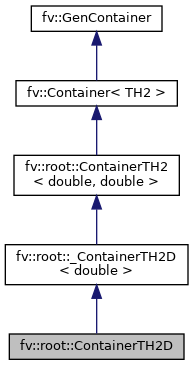
\includegraphics[width=217pt]{classfv_1_1root_1_1ContainerTH2D__inherit__graph}
\end{center}
\end{figure}


Collaboration diagram for fv\+:\+:root\+:\+:Container\+T\+H2D\+:
\nopagebreak
\begin{figure}[H]
\begin{center}
\leavevmode
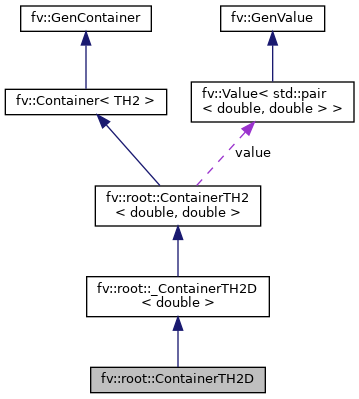
\includegraphics[width=342pt]{classfv_1_1root_1_1ContainerTH2D__coll__graph}
\end{center}
\end{figure}
\subsection*{Private Member Functions}
\begin{DoxyCompactItemize}
\item 
\hypertarget{classfv_1_1root_1_1ContainerTH2D_ac61ace3c44f5f371b69edc7394fba54f}{}\label{classfv_1_1root_1_1ContainerTH2D_ac61ace3c44f5f371b69edc7394fba54f} 
void {\bfseries \+\_\+do\+\_\+fill} (std\+::pair$<$ double, double $>$ \&val)
\end{DoxyCompactItemize}
\subsection*{Additional Inherited Members}


The documentation for this class was generated from the following file\+:\begin{DoxyCompactItemize}
\item 
/home/caleb/\+Sources/\+T\+T\+T\+T/filval\+\_\+root/container.\+hpp\end{DoxyCompactItemize}

\hypertarget{classfv_1_1root_1_1ContainerTH2DMany}{}\section{fv\+:\+:root\+:\+:Container\+T\+H2\+D\+Many Class Reference}
\label{classfv_1_1root_1_1ContainerTH2DMany}\index{fv\+::root\+::\+Container\+T\+H2\+D\+Many@{fv\+::root\+::\+Container\+T\+H2\+D\+Many}}


Inheritance diagram for fv\+:\+:root\+:\+:Container\+T\+H2\+D\+Many\+:
\nopagebreak
\begin{figure}[H]
\begin{center}
\leavevmode
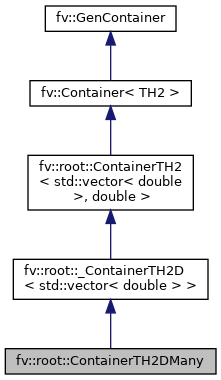
\includegraphics[width=238pt]{classfv_1_1root_1_1ContainerTH2DMany__inherit__graph}
\end{center}
\end{figure}


Collaboration diagram for fv\+:\+:root\+:\+:Container\+T\+H2\+D\+Many\+:
\nopagebreak
\begin{figure}[H]
\begin{center}
\leavevmode
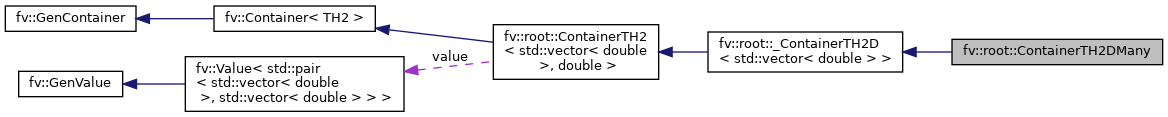
\includegraphics[width=350pt]{classfv_1_1root_1_1ContainerTH2DMany__coll__graph}
\end{center}
\end{figure}
\subsection*{Private Member Functions}
\begin{DoxyCompactItemize}
\item 
\hypertarget{classfv_1_1root_1_1ContainerTH2DMany_a94e7713ed35518d23ac7608c1119caed}{}\label{classfv_1_1root_1_1ContainerTH2DMany_a94e7713ed35518d23ac7608c1119caed} 
void {\bfseries \+\_\+do\+\_\+fill} (std\+::pair$<$ std\+::vector$<$ double $>$, std\+::vector$<$ double $>$$>$ \&val)
\end{DoxyCompactItemize}
\subsection*{Additional Inherited Members}


The documentation for this class was generated from the following file\+:\begin{DoxyCompactItemize}
\item 
/home/caleb/\+Sources/\+T\+T\+T\+T/filval\+\_\+root/container.\+hpp\end{DoxyCompactItemize}

\hypertarget{classfv_1_1root_1_1ContainerTH2F}{}\section{fv\+:\+:root\+:\+:Container\+T\+H2F Class Reference}
\label{classfv_1_1root_1_1ContainerTH2F}\index{fv\+::root\+::\+Container\+T\+H2F@{fv\+::root\+::\+Container\+T\+H2F}}


Inheritance diagram for fv\+:\+:root\+:\+:Container\+T\+H2F\+:
\nopagebreak
\begin{figure}[H]
\begin{center}
\leavevmode
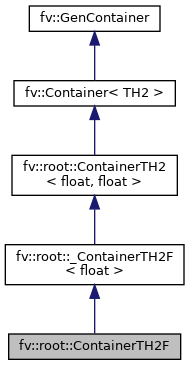
\includegraphics[width=214pt]{classfv_1_1root_1_1ContainerTH2F__inherit__graph}
\end{center}
\end{figure}


Collaboration diagram for fv\+:\+:root\+:\+:Container\+T\+H2F\+:
\nopagebreak
\begin{figure}[H]
\begin{center}
\leavevmode
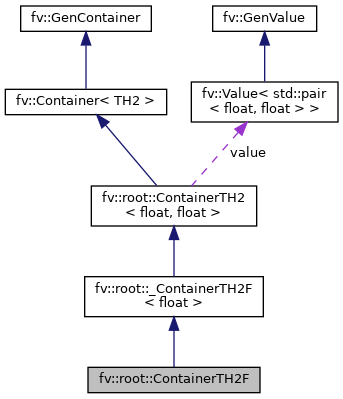
\includegraphics[width=330pt]{classfv_1_1root_1_1ContainerTH2F__coll__graph}
\end{center}
\end{figure}
\subsection*{Private Member Functions}
\begin{DoxyCompactItemize}
\item 
\hypertarget{classfv_1_1root_1_1ContainerTH2F_a47270db4e46873e22915dd0281c1d669}{}\label{classfv_1_1root_1_1ContainerTH2F_a47270db4e46873e22915dd0281c1d669} 
void {\bfseries \+\_\+do\+\_\+fill} (std\+::pair$<$ float, float $>$ \&val)
\end{DoxyCompactItemize}
\subsection*{Additional Inherited Members}


The documentation for this class was generated from the following file\+:\begin{DoxyCompactItemize}
\item 
/home/caleb/\+Sources/\+T\+T\+T\+T/filval\+\_\+root/container.\+hpp\end{DoxyCompactItemize}

\hypertarget{classfv_1_1root_1_1ContainerTH2FMany}{}\section{fv\+:\+:root\+:\+:Container\+T\+H2\+F\+Many Class Reference}
\label{classfv_1_1root_1_1ContainerTH2FMany}\index{fv\+::root\+::\+Container\+T\+H2\+F\+Many@{fv\+::root\+::\+Container\+T\+H2\+F\+Many}}


Inheritance diagram for fv\+:\+:root\+:\+:Container\+T\+H2\+F\+Many\+:
\nopagebreak
\begin{figure}[H]
\begin{center}
\leavevmode
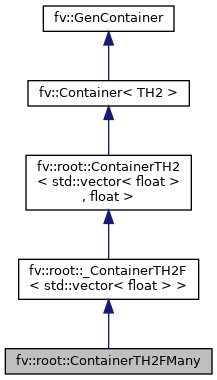
\includegraphics[width=235pt]{classfv_1_1root_1_1ContainerTH2FMany__inherit__graph}
\end{center}
\end{figure}


Collaboration diagram for fv\+:\+:root\+:\+:Container\+T\+H2\+F\+Many\+:
\nopagebreak
\begin{figure}[H]
\begin{center}
\leavevmode
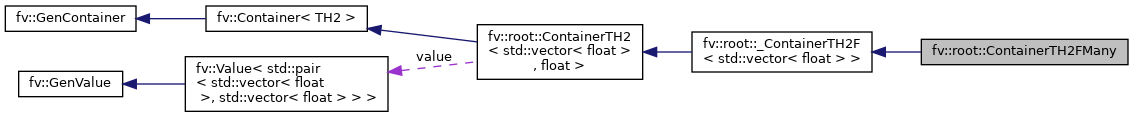
\includegraphics[width=350pt]{classfv_1_1root_1_1ContainerTH2FMany__coll__graph}
\end{center}
\end{figure}
\subsection*{Private Member Functions}
\begin{DoxyCompactItemize}
\item 
\hypertarget{classfv_1_1root_1_1ContainerTH2FMany_a17efa27a901c971bfda82cf218d63264}{}\label{classfv_1_1root_1_1ContainerTH2FMany_a17efa27a901c971bfda82cf218d63264} 
void {\bfseries \+\_\+do\+\_\+fill} (std\+::pair$<$ std\+::vector$<$ float $>$, std\+::vector$<$ float $>$$>$ \&val)
\end{DoxyCompactItemize}
\subsection*{Additional Inherited Members}


The documentation for this class was generated from the following file\+:\begin{DoxyCompactItemize}
\item 
/home/caleb/\+Sources/\+T\+T\+T\+T/filval\+\_\+root/container.\+hpp\end{DoxyCompactItemize}

\hypertarget{classfv_1_1root_1_1ContainerTH2I}{}\section{fv\+:\+:root\+:\+:Container\+T\+H2I Class Reference}
\label{classfv_1_1root_1_1ContainerTH2I}\index{fv\+::root\+::\+Container\+T\+H2I@{fv\+::root\+::\+Container\+T\+H2I}}


Inheritance diagram for fv\+:\+:root\+:\+:Container\+T\+H2I\+:
\nopagebreak
\begin{figure}[H]
\begin{center}
\leavevmode
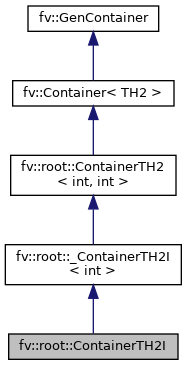
\includegraphics[width=212pt]{classfv_1_1root_1_1ContainerTH2I__inherit__graph}
\end{center}
\end{figure}


Collaboration diagram for fv\+:\+:root\+:\+:Container\+T\+H2I\+:
\nopagebreak
\begin{figure}[H]
\begin{center}
\leavevmode
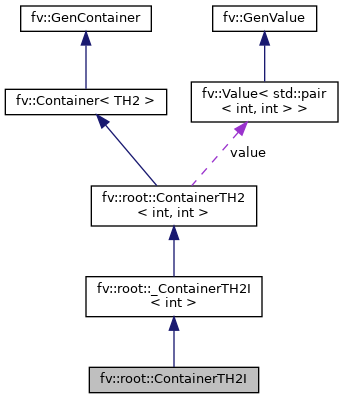
\includegraphics[width=330pt]{classfv_1_1root_1_1ContainerTH2I__coll__graph}
\end{center}
\end{figure}
\subsection*{Private Member Functions}
\begin{DoxyCompactItemize}
\item 
\hypertarget{classfv_1_1root_1_1ContainerTH2I_a3607e20e3088a42b955c211587bba622}{}\label{classfv_1_1root_1_1ContainerTH2I_a3607e20e3088a42b955c211587bba622} 
void {\bfseries \+\_\+do\+\_\+fill} (std\+::pair$<$ int, int $>$ \&val)
\end{DoxyCompactItemize}
\subsection*{Additional Inherited Members}


The documentation for this class was generated from the following file\+:\begin{DoxyCompactItemize}
\item 
/home/caleb/\+Sources/\+T\+T\+T\+T/filval\+\_\+root/container.\+hpp\end{DoxyCompactItemize}

\hypertarget{classfv_1_1root_1_1ContainerTH2IMany}{}\section{fv\+:\+:root\+:\+:Container\+T\+H2\+I\+Many Class Reference}
\label{classfv_1_1root_1_1ContainerTH2IMany}\index{fv\+::root\+::\+Container\+T\+H2\+I\+Many@{fv\+::root\+::\+Container\+T\+H2\+I\+Many}}


Inheritance diagram for fv\+:\+:root\+:\+:Container\+T\+H2\+I\+Many\+:
\nopagebreak
\begin{figure}[H]
\begin{center}
\leavevmode
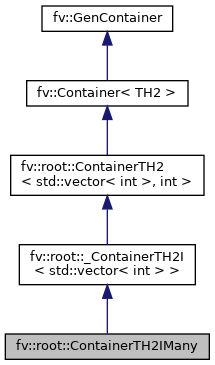
\includegraphics[width=233pt]{classfv_1_1root_1_1ContainerTH2IMany__inherit__graph}
\end{center}
\end{figure}


Collaboration diagram for fv\+:\+:root\+:\+:Container\+T\+H2\+I\+Many\+:
\nopagebreak
\begin{figure}[H]
\begin{center}
\leavevmode
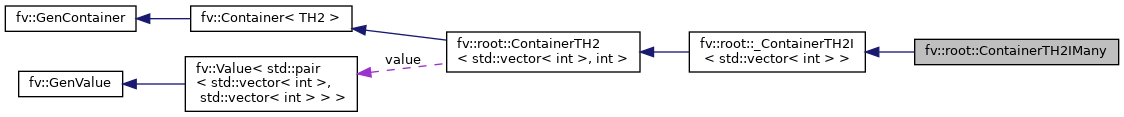
\includegraphics[width=350pt]{classfv_1_1root_1_1ContainerTH2IMany__coll__graph}
\end{center}
\end{figure}
\subsection*{Private Member Functions}
\begin{DoxyCompactItemize}
\item 
\hypertarget{classfv_1_1root_1_1ContainerTH2IMany_accb852d9d896903c367fb949cf7f828c}{}\label{classfv_1_1root_1_1ContainerTH2IMany_accb852d9d896903c367fb949cf7f828c} 
void {\bfseries \+\_\+do\+\_\+fill} (std\+::pair$<$ std\+::vector$<$ int $>$, std\+::vector$<$ int $>$$>$ \&val)
\end{DoxyCompactItemize}
\subsection*{Additional Inherited Members}


The documentation for this class was generated from the following file\+:\begin{DoxyCompactItemize}
\item 
/home/caleb/\+Sources/\+T\+T\+T\+T/filval\+\_\+root/container.\+hpp\end{DoxyCompactItemize}

\hypertarget{classfv_1_1ContainerVector}{}\section{fv\+:\+:Container\+Vector$<$ T $>$ Class Template Reference}
\label{classfv_1_1ContainerVector}\index{fv\+::\+Container\+Vector$<$ T $>$@{fv\+::\+Container\+Vector$<$ T $>$}}


Inheritance diagram for fv\+:\+:Container\+Vector$<$ T $>$\+:
\nopagebreak
\begin{figure}[H]
\begin{center}
\leavevmode
\includegraphics[width=218pt]{classfv_1_1ContainerVector__inherit__graph}
\end{center}
\end{figure}


Collaboration diagram for fv\+:\+:Container\+Vector$<$ T $>$\+:
\nopagebreak
\begin{figure}[H]
\begin{center}
\leavevmode
\includegraphics[width=218pt]{classfv_1_1ContainerVector__coll__graph}
\end{center}
\end{figure}
\subsection*{Public Member Functions}
\begin{DoxyCompactItemize}
\item 
\hypertarget{classfv_1_1ContainerVector_a8bfcac1f432f1b61184f5adb1c411cfd}{}\label{classfv_1_1ContainerVector_a8bfcac1f432f1b61184f5adb1c411cfd} 
{\bfseries Container\+Vector} (const std\+::string \&name, std\+::vector$<$ T $>$ $\ast$container, \hyperlink{classfv_1_1Value}{Value}$<$ T $>$ $\ast$value)
\item 
\hypertarget{classfv_1_1ContainerVector_ac84c934248630971b883a1cf1609cd21}{}\label{classfv_1_1ContainerVector_ac84c934248630971b883a1cf1609cd21} 
{\bfseries Container\+Vector} (const std\+::string \&name, \hyperlink{classfv_1_1Value}{Value}$<$ T $>$ $\ast$value)
\item 
\hypertarget{classfv_1_1ContainerVector_abda11b97b7f06b3b2c61099b1e8a4410}{}\label{classfv_1_1ContainerVector_abda11b97b7f06b3b2c61099b1e8a4410} 
void {\bfseries save\+\_\+as} (const std\+::string \&fname)
\item 
\hypertarget{classfv_1_1ContainerVector_a25d5275136d098d96fe2a43266dbc2c6}{}\label{classfv_1_1ContainerVector_a25d5275136d098d96fe2a43266dbc2c6} 
virtual void {\bfseries save} ()
\end{DoxyCompactItemize}
\subsection*{Private Member Functions}
\begin{DoxyCompactItemize}
\item 
\hypertarget{classfv_1_1ContainerVector_a7d022ea13bcd5db0693b0b9e6172c1df}{}\label{classfv_1_1ContainerVector_a7d022ea13bcd5db0693b0b9e6172c1df} 
void {\bfseries \+\_\+fill} ()
\end{DoxyCompactItemize}
\subsection*{Private Attributes}
\begin{DoxyCompactItemize}
\item 
\hypertarget{classfv_1_1ContainerVector_a61f625e896ebdbe08949a5fad08dafab}{}\label{classfv_1_1ContainerVector_a61f625e896ebdbe08949a5fad08dafab} 
\hyperlink{classfv_1_1Value}{Value}$<$ T $>$ $\ast$ {\bfseries value}
\end{DoxyCompactItemize}
\subsection*{Additional Inherited Members}


The documentation for this class was generated from the following file\+:\begin{DoxyCompactItemize}
\item 
/home/caleb/\+Sources/\+T\+T\+T\+T/filval/container.\+hpp\end{DoxyCompactItemize}

\hypertarget{classfv_1_1Count}{}\section{fv\+:\+:Count$<$ T $>$ Class Template Reference}
\label{classfv_1_1Count}\index{fv\+::\+Count$<$ T $>$@{fv\+::\+Count$<$ T $>$}}


Inheritance diagram for fv\+:\+:Count$<$ T $>$\+:
\nopagebreak
\begin{figure}[H]
\begin{center}
\leavevmode
\includegraphics[width=212pt]{classfv_1_1Count__inherit__graph}
\end{center}
\end{figure}


Collaboration diagram for fv\+:\+:Count$<$ T $>$\+:
\nopagebreak
\begin{figure}[H]
\begin{center}
\leavevmode
\includegraphics[width=350pt]{classfv_1_1Count__coll__graph}
\end{center}
\end{figure}
\subsection*{Public Member Functions}
\begin{DoxyCompactItemize}
\item 
\hypertarget{classfv_1_1Count_a8d737015331b4bdff6614118c957bfb6}{}\label{classfv_1_1Count_a8d737015331b4bdff6614118c957bfb6} 
{\bfseries Count} (\hyperlink{classfv_1_1Function}{Function}$<$ bool(T)$>$ \&selector, \hyperlink{classfv_1_1Value}{Value}$<$ std\+::vector$<$ T $>$$>$ $\ast$v, const std\+::string alias=\char`\"{}\char`\"{})
\item 
\hypertarget{classfv_1_1Count_a1ea910638294d8a70c6892ac93b23654}{}\label{classfv_1_1Count_a1ea910638294d8a70c6892ac93b23654} 
{\bfseries Count} (\hyperlink{classfv_1_1Function}{Function}$<$ bool(T)$>$ \&selector, const std\+::string \&v\+\_\+name, const std\+::string alias=\char`\"{}\char`\"{})
\end{DoxyCompactItemize}
\subsection*{Private Member Functions}
\begin{DoxyCompactItemize}
\item 
void \hyperlink{classfv_1_1Count_afff1c16a8747a82db1cc1c8248c56a08}{update\+\_\+value} ()
\begin{DoxyCompactList}\small\item\em Updates the internal value. \end{DoxyCompactList}\end{DoxyCompactItemize}
\subsection*{Private Attributes}
\begin{DoxyCompactItemize}
\item 
\hypertarget{classfv_1_1Count_a1dbfccc8020b2c41adcedc5e449ff3be}{}\label{classfv_1_1Count_a1dbfccc8020b2c41adcedc5e449ff3be} 
\hyperlink{classfv_1_1Function}{Function}$<$ bool(T)$>$ \& {\bfseries selector}
\item 
\hypertarget{classfv_1_1Count_a3bb2f22dc995dc833f513805128e3a44}{}\label{classfv_1_1Count_a3bb2f22dc995dc833f513805128e3a44} 
\hyperlink{classfv_1_1Value}{Value}$<$ std\+::vector$<$ T $>$ $>$ $\ast$ {\bfseries v}
\end{DoxyCompactItemize}
\subsection*{Additional Inherited Members}


\subsection{Member Function Documentation}
\hypertarget{classfv_1_1Count_afff1c16a8747a82db1cc1c8248c56a08}{}\label{classfv_1_1Count_afff1c16a8747a82db1cc1c8248c56a08} 
\index{fv\+::\+Count@{fv\+::\+Count}!update\+\_\+value@{update\+\_\+value}}
\index{update\+\_\+value@{update\+\_\+value}!fv\+::\+Count@{fv\+::\+Count}}
\subsubsection{\texorpdfstring{update\+\_\+value()}{update\_value()}}
{\footnotesize\ttfamily template$<$typename T $>$ \\
void \hyperlink{classfv_1_1Count}{fv\+::\+Count}$<$ T $>$\+::update\+\_\+value (\begin{DoxyParamCaption}{ }\end{DoxyParamCaption})\hspace{0.3cm}{\ttfamily [inline]}, {\ttfamily [private]}, {\ttfamily [virtual]}}



Updates the internal value. 

This function should be overridden by any child class to do the actual work of updating value based on whatever rules the class chooses. Normally, this consists of geting the values from some associated \hyperlink{classfv_1_1Value}{Value} objects, doing some calculation on them, and storing the result in value. 

Implements \hyperlink{classfv_1_1DerivedValue_ae59e80a98eb74b95d8961bfe12ee5ec2}{fv\+::\+Derived\+Value$<$ int $>$}.

Here is the call graph for this function\+:
\nopagebreak
\begin{figure}[H]
\begin{center}
\leavevmode
\includegraphics[width=350pt]{classfv_1_1Count_afff1c16a8747a82db1cc1c8248c56a08_cgraph}
\end{center}
\end{figure}


The documentation for this class was generated from the following file\+:\begin{DoxyCompactItemize}
\item 
/home/caleb/\+Sources/\+T\+T\+T\+T/filval/\hyperlink{value_8hpp}{value.\+hpp}\end{DoxyCompactItemize}

\hypertarget{classfv_1_1DataSet}{}\section{fv\+:\+:Data\+Set Class Reference}
\label{classfv_1_1DataSet}\index{fv\+::\+Data\+Set@{fv\+::\+Data\+Set}}
\subsection*{Public Member Functions}
\begin{DoxyCompactItemize}
\item 
\hypertarget{classfv_1_1DataSet_a77975c8e8f46b4c9b9dd6f5a83fd05ed}{}\label{classfv_1_1DataSet_a77975c8e8f46b4c9b9dd6f5a83fd05ed} 
void {\bfseries process} (bool silent=false)
\item 
\hypertarget{classfv_1_1DataSet_a115ab5a200c64b8df54d17d0dd6524cf}{}\label{classfv_1_1DataSet_a115ab5a200c64b8df54d17d0dd6524cf} 
virtual void {\bfseries save\+\_\+all} ()
\item 
\hypertarget{classfv_1_1DataSet_aa9b414d264b13ab78c5153fbaea13c89}{}\label{classfv_1_1DataSet_aa9b414d264b13ab78c5153fbaea13c89} 
void {\bfseries register\+\_\+container} (\hyperlink{classfv_1_1GenContainer}{Gen\+Container} $\ast$container)
\item 
\hypertarget{classfv_1_1DataSet_a045e7756fe5970cdaab953f12af25de5}{}\label{classfv_1_1DataSet_a045e7756fe5970cdaab953f12af25de5} 
\hyperlink{classfv_1_1GenContainer}{Gen\+Container} $\ast$ {\bfseries get\+\_\+container} (std\+::string container\+\_\+name)
\end{DoxyCompactItemize}
\subsection*{Protected Member Functions}
\begin{DoxyCompactItemize}
\item 
\hypertarget{classfv_1_1DataSet_ac11e2a57a0712aa572f398f275f5821b}{}\label{classfv_1_1DataSet_ac11e2a57a0712aa572f398f275f5821b} 
virtual bool {\bfseries load\+\_\+next} ()=0
\item 
\hypertarget{classfv_1_1DataSet_a54bec77bf1597c504c1f3e56c076110f}{}\label{classfv_1_1DataSet_a54bec77bf1597c504c1f3e56c076110f} 
virtual int {\bfseries get\+\_\+events} ()=0
\item 
\hypertarget{classfv_1_1DataSet_a0e69eac5f063215fc00a3f387cb8e682}{}\label{classfv_1_1DataSet_a0e69eac5f063215fc00a3f387cb8e682} 
virtual int {\bfseries get\+\_\+current\+\_\+event} ()=0
\end{DoxyCompactItemize}
\subsection*{Protected Attributes}
\begin{DoxyCompactItemize}
\item 
\hypertarget{classfv_1_1DataSet_a8bfd9b92632c1ec6c292b7a97578b75c}{}\label{classfv_1_1DataSet_a8bfd9b92632c1ec6c292b7a97578b75c} 
Container\+Set {\bfseries containers}
\end{DoxyCompactItemize}
\subsection*{Private Member Functions}
\begin{DoxyCompactItemize}
\item 
\hypertarget{classfv_1_1DataSet_aaa8a985360a4848304aa3c9ed39d11ff}{}\label{classfv_1_1DataSet_aaa8a985360a4848304aa3c9ed39d11ff} 
void {\bfseries summary} ()
\end{DoxyCompactItemize}


The documentation for this class was generated from the following file\+:\begin{DoxyCompactItemize}
\item 
/home/caleb/\+Sources/\+T\+T\+T\+T/filval/dataset.\+hpp\end{DoxyCompactItemize}

\hypertarget{classfv_1_1DerivedValue}{}\section{fv\+:\+:Derived\+Value$<$ T $>$ Class Template Reference}
\label{classfv_1_1DerivedValue}\index{fv\+::\+Derived\+Value$<$ T $>$@{fv\+::\+Derived\+Value$<$ T $>$}}


A generic, derived, value.  




{\ttfamily \#include $<$value.\+hpp$>$}



Inheritance diagram for fv\+:\+:Derived\+Value$<$ T $>$\+:
\nopagebreak
\begin{figure}[H]
\begin{center}
\leavevmode
\includegraphics[width=350pt]{classfv_1_1DerivedValue__inherit__graph}
\end{center}
\end{figure}


Collaboration diagram for fv\+:\+:Derived\+Value$<$ T $>$\+:
\nopagebreak
\begin{figure}[H]
\begin{center}
\leavevmode
\includegraphics[width=243pt]{classfv_1_1DerivedValue__coll__graph}
\end{center}
\end{figure}
\subsection*{Public Member Functions}
\begin{DoxyCompactItemize}
\item 
\hypertarget{classfv_1_1DerivedValue_a00219a17112600afdc060d67d6f95b21}{}\label{classfv_1_1DerivedValue_a00219a17112600afdc060d67d6f95b21} 
{\bfseries Derived\+Value} (const std\+::string \&\hyperlink{classfv_1_1GenValue_a610f89ee441eaad4c9e78f74d6bde93b}{name}, const std\+::string \&alias=\char`\"{}\char`\"{})
\item 
\hypertarget{classfv_1_1DerivedValue_a39970158aa8f6eb062a28037df6e2128}{}\label{classfv_1_1DerivedValue_a39970158aa8f6eb062a28037df6e2128} 
T \& \hyperlink{classfv_1_1DerivedValue_a39970158aa8f6eb062a28037df6e2128}{get\+\_\+value} ()
\begin{DoxyCompactList}\small\item\em Calculate, if necessary, and return the value held by this object. \end{DoxyCompactList}\end{DoxyCompactItemize}
\subsection*{Protected Member Functions}
\begin{DoxyCompactItemize}
\item 
virtual void \hyperlink{classfv_1_1DerivedValue_ae59e80a98eb74b95d8961bfe12ee5ec2}{update\+\_\+value} ()=0
\begin{DoxyCompactList}\small\item\em Updates the internal value. \end{DoxyCompactList}\end{DoxyCompactItemize}
\subsection*{Protected Attributes}
\begin{DoxyCompactItemize}
\item 
\hypertarget{classfv_1_1DerivedValue_aeb7ff5d17ad44b2040fc9930bbcc2c7a}{}\label{classfv_1_1DerivedValue_aeb7ff5d17ad44b2040fc9930bbcc2c7a} 
T {\bfseries value}
\item 
\hypertarget{classfv_1_1DerivedValue_aafa55adbb38dc7fe210ea15e920515dc}{}\label{classfv_1_1DerivedValue_aafa55adbb38dc7fe210ea15e920515dc} 
bool {\bfseries value\+\_\+valid}
\end{DoxyCompactItemize}
\subsection*{Private Member Functions}
\begin{DoxyCompactItemize}
\item 
void \hyperlink{classfv_1_1DerivedValue_a5c296d4f3171797f31a3fab002dececa}{\+\_\+reset} ()
\begin{DoxyCompactList}\small\item\em Mark the internal value as invalid. \end{DoxyCompactList}\end{DoxyCompactItemize}
\subsection*{Additional Inherited Members}


\subsection{Detailed Description}
\subsubsection*{template$<$typename T$>$\newline
class fv\+::\+Derived\+Value$<$ T $>$}

A generic, derived, value. 

A \hyperlink{classfv_1_1DerivedValue}{Derived\+Value} is generally defined as some function of other \hyperlink{classfv_1_1Value}{Value} objects. For example, a \hyperlink{classfv_1_1Pair}{Pair} is a function of two other \hyperlink{classfv_1_1Value}{Value} objects that makes a pair of them. Note that these other \hyperlink{classfv_1_1Value}{Value} objects are free to be either Observed\+Values or other Derived\+Values.

It is desireable from a performance standpoint that each \hyperlink{classfv_1_1DerivedValue}{Derived\+Value} be calculated no more than once per observation. Therefore, when a get\+\_\+value is called on a \hyperlink{classfv_1_1DerivedValue}{Derived\+Value}, it first checks whether the value that it holds is {\bfseries valid}, meaning it has already been calculated for this observation. If so, it simply returns the value. If not, the update\+\_\+value function is called to calculate the value. and then the newly calculated value is marked as valid and returned. 

\subsection{Member Function Documentation}
\hypertarget{classfv_1_1DerivedValue_a5c296d4f3171797f31a3fab002dececa}{}\label{classfv_1_1DerivedValue_a5c296d4f3171797f31a3fab002dececa} 
\index{fv\+::\+Derived\+Value@{fv\+::\+Derived\+Value}!\+\_\+reset@{\+\_\+reset}}
\index{\+\_\+reset@{\+\_\+reset}!fv\+::\+Derived\+Value@{fv\+::\+Derived\+Value}}
\subsubsection{\texorpdfstring{\+\_\+reset()}{\_reset()}}
{\footnotesize\ttfamily template$<$typename T$>$ \\
void \hyperlink{classfv_1_1DerivedValue}{fv\+::\+Derived\+Value}$<$ T $>$\+::\+\_\+reset (\begin{DoxyParamCaption}{ }\end{DoxyParamCaption})\hspace{0.3cm}{\ttfamily [inline]}, {\ttfamily [private]}, {\ttfamily [virtual]}}



Mark the internal value as invalid. 

This is needed for \hyperlink{classfv_1_1DerivedValue}{Derived\+Value} to force a recalculation of the internal value when a new observation is loaded into memory. It is called automatically for all \hyperlink{classfv_1_1GenValue}{Gen\+Value} objects when reset is called. 

Implements \hyperlink{classfv_1_1GenValue_a26160e53542b728f9e0c11495dce3c20}{fv\+::\+Gen\+Value}.

\hypertarget{classfv_1_1DerivedValue_ae59e80a98eb74b95d8961bfe12ee5ec2}{}\label{classfv_1_1DerivedValue_ae59e80a98eb74b95d8961bfe12ee5ec2} 
\index{fv\+::\+Derived\+Value@{fv\+::\+Derived\+Value}!update\+\_\+value@{update\+\_\+value}}
\index{update\+\_\+value@{update\+\_\+value}!fv\+::\+Derived\+Value@{fv\+::\+Derived\+Value}}
\subsubsection{\texorpdfstring{update\+\_\+value()}{update\_value()}}
{\footnotesize\ttfamily template$<$typename T$>$ \\
virtual void \hyperlink{classfv_1_1DerivedValue}{fv\+::\+Derived\+Value}$<$ T $>$\+::update\+\_\+value (\begin{DoxyParamCaption}{ }\end{DoxyParamCaption})\hspace{0.3cm}{\ttfamily [protected]}, {\ttfamily [pure virtual]}}



Updates the internal value. 

This function should be overridden by any child class to do the actual work of updating value based on whatever rules the class chooses. Normally, this consists of geting the values from some associated \hyperlink{classfv_1_1Value}{Value} objects, doing some calculation on them, and storing the result in value. 

Implemented in \hyperlink{classfv_1_1ConstantValue_a6581e7fb69c082c07c9714138063b320}{fv\+::\+Constant\+Value$<$ T $>$}, \hyperlink{classfv_1_1PointerValue_a81e39d040919be39c37f845a27343f3e}{fv\+::\+Pointer\+Value$<$ T $>$}, \hyperlink{classfv_1_1BoundValue_a51ba914f1eac694af4264d62785282a1}{fv\+::\+Bound\+Value$<$ T $>$}, \hyperlink{classfv_1_1ReduceIndex_a462bffebe2a93c940aca526566d48e37}{fv\+::\+Reduce\+Index$<$ T $>$}, \hyperlink{classfv_1_1Reduce_ab0809c4ab1884b84a7f88e005ade76a5}{fv\+::\+Reduce$<$ T $>$}, \hyperlink{classfv_1_1Count_afff1c16a8747a82db1cc1c8248c56a08}{fv\+::\+Count$<$ T $>$}, \hyperlink{classfv_1_1ZipMapFour_a812747fdc043c776951ceb93a1085915}{fv\+::\+Zip\+Map\+Four$<$ R, T $>$}, \hyperlink{classfv_1_1Pair_ab3225f03f49240fc1547a5005f57b864}{fv\+::\+Pair$<$ T1, T2 $>$}, \hyperlink{classfv_1_1WrapperVector_a2ee99bc4425642d209df7b48ee2ada95}{fv\+::\+Wrapper\+Vector$<$ T $>$}, \hyperlink{classfv_1_1Filter_ab3ed620127ccb32f75bc5e78bc8a60b3}{fv\+::\+Filter}, \hyperlink{classfv_1_1root_1_1LorentzVectorEnergy_aa69384d1af673c327daae869d5977981}{fv\+::root\+::\+Lorentz\+Vector\+Energy}, \hyperlink{classfv_1_1root_1_1LorentzVector_aeb17320a2024bd189dad4117cf1f54fb}{fv\+::root\+::\+Lorentz\+Vector}, and \hyperlink{classfv_1_1root_1_1MassFilter_a1a8b086086e1220bc352523184d3f1c2}{fv\+::root\+::\+Mass\+Filter}.



The documentation for this class was generated from the following file\+:\begin{DoxyCompactItemize}
\item 
/home/caleb/\+Sources/\+T\+T\+T\+T/filval/\hyperlink{value_8hpp}{value.\+hpp}\end{DoxyCompactItemize}

\hypertarget{classfv_1_1ElementOf}{}\section{fv\+:\+:Element\+Of$<$ T $>$ Class Template Reference}
\label{classfv_1_1ElementOf}\index{fv\+::\+Element\+Of$<$ T $>$@{fv\+::\+Element\+Of$<$ T $>$}}


Extract the element at a specific index from a vector.  




{\ttfamily \#include $<$value.\+hpp$>$}



Inheritance diagram for fv\+:\+:Element\+Of$<$ T $>$\+:
\nopagebreak
\begin{figure}[H]
\begin{center}
\leavevmode
\includegraphics[width=205pt]{classfv_1_1ElementOf__inherit__graph}
\end{center}
\end{figure}


Collaboration diagram for fv\+:\+:Element\+Of$<$ T $>$\+:
\nopagebreak
\begin{figure}[H]
\begin{center}
\leavevmode
\includegraphics[width=350pt]{classfv_1_1ElementOf__coll__graph}
\end{center}
\end{figure}
\subsection*{Public Member Functions}
\begin{DoxyCompactItemize}
\item 
\hypertarget{classfv_1_1ElementOf_ae43a7e9890d411b6cbfa28232f375695}{}\label{classfv_1_1ElementOf_ae43a7e9890d411b6cbfa28232f375695} 
{\bfseries Element\+Of} (\hyperlink{classfv_1_1Value}{Value}$<$ int $>$ $\ast$index, const std\+::string \&v\+\_\+name, const std\+::string alias=\char`\"{}\char`\"{})
\item 
\hypertarget{classfv_1_1ElementOf_acce67227b0a453836636433288fc85b3}{}\label{classfv_1_1ElementOf_acce67227b0a453836636433288fc85b3} 
{\bfseries Element\+Of} (const std\+::string \&\hyperlink{classfv_1_1GenValue_a610f89ee441eaad4c9e78f74d6bde93b}{name}, int index, const std\+::string \&v\+\_\+name, const std\+::string alias=\char`\"{}\char`\"{})
\end{DoxyCompactItemize}
\subsection*{Additional Inherited Members}


\subsection{Detailed Description}
\subsubsection*{template$<$typename T$>$\newline
class fv\+::\+Element\+Of$<$ T $>$}

Extract the element at a specific index from a vector. 

The documentation for this class was generated from the following file\+:\begin{DoxyCompactItemize}
\item 
/home/caleb/\+Sources/\+T\+T\+T\+T/filval/\hyperlink{value_8hpp}{value.\+hpp}\end{DoxyCompactItemize}

\hypertarget{classfv_1_1Filter}{}\section{fv\+:\+:Filter Class Reference}
\label{classfv_1_1Filter}\index{fv\+::\+Filter@{fv\+::\+Filter}}


Inheritance diagram for fv\+:\+:Filter\+:
\nopagebreak
\begin{figure}[H]
\begin{center}
\leavevmode
\includegraphics[width=320pt]{classfv_1_1Filter__inherit__graph}
\end{center}
\end{figure}


Collaboration diagram for fv\+:\+:Filter\+:
\nopagebreak
\begin{figure}[H]
\begin{center}
\leavevmode
\includegraphics[width=350pt]{classfv_1_1Filter__coll__graph}
\end{center}
\end{figure}
\subsection*{Public Member Functions}
\begin{DoxyCompactItemize}
\item 
\hypertarget{classfv_1_1Filter_a7bb0f3ff6419e820a24be78d48b8769d}{}\label{classfv_1_1Filter_a7bb0f3ff6419e820a24be78d48b8769d} 
{\bfseries Filter} (const std\+::string \&\hyperlink{classfv_1_1GenValue_a610f89ee441eaad4c9e78f74d6bde93b}{name}, std\+::function$<$ bool()$>$ filter\+\_\+function, const std\+::string \&impl=\char`\"{}\char`\"{})
\item 
\hypertarget{classfv_1_1Filter_ae787cf77d98ac3604cba541afad0b351}{}\label{classfv_1_1Filter_ae787cf77d98ac3604cba541afad0b351} 
\hyperlink{classfv_1_1Filter}{Filter} $\ast$ \hyperlink{classfv_1_1Filter_ae787cf77d98ac3604cba541afad0b351}{operator$\ast$} (\hyperlink{classfv_1_1Filter}{Filter} $\ast$f)
\begin{DoxyCompactList}\small\item\em Return a new filter that is the conjuction of the two source filters. \end{DoxyCompactList}\item 
\hypertarget{classfv_1_1Filter_aea96a9a83e172b7fdb64be78b0b3fffe}{}\label{classfv_1_1Filter_aea96a9a83e172b7fdb64be78b0b3fffe} 
\hyperlink{classfv_1_1Filter}{Filter} $\ast$ \hyperlink{classfv_1_1Filter_aea96a9a83e172b7fdb64be78b0b3fffe}{operator+} (\hyperlink{classfv_1_1Filter}{Filter} $\ast$f)
\begin{DoxyCompactList}\small\item\em Return a new filter that is the disjunction of the two source filters. \end{DoxyCompactList}\item 
\hypertarget{classfv_1_1Filter_abb459c8bbb3b51cd85ab5a0f7b2f154d}{}\label{classfv_1_1Filter_abb459c8bbb3b51cd85ab5a0f7b2f154d} 
\hyperlink{classfv_1_1Filter}{Filter} $\ast$ \hyperlink{classfv_1_1Filter_abb459c8bbb3b51cd85ab5a0f7b2f154d}{operator!} ()
\begin{DoxyCompactList}\small\item\em Return a new filter that is the negation of the source filter. \end{DoxyCompactList}\end{DoxyCompactItemize}
\subsection*{Private Member Functions}
\begin{DoxyCompactItemize}
\item 
void \hyperlink{classfv_1_1Filter_ab3ed620127ccb32f75bc5e78bc8a60b3}{update\+\_\+value} ()
\begin{DoxyCompactList}\small\item\em Updates the internal value. \end{DoxyCompactList}\end{DoxyCompactItemize}
\subsection*{Private Attributes}
\begin{DoxyCompactItemize}
\item 
\hypertarget{classfv_1_1Filter_a0c8d620dcf75608a8afaf2e34c773e3f}{}\label{classfv_1_1Filter_a0c8d620dcf75608a8afaf2e34c773e3f} 
\hyperlink{classfv_1_1Function}{Function}$<$ bool()$>$ \& {\bfseries filter\+\_\+function}
\end{DoxyCompactItemize}
\subsection*{Additional Inherited Members}


\subsection{Member Function Documentation}
\hypertarget{classfv_1_1Filter_ab3ed620127ccb32f75bc5e78bc8a60b3}{}\label{classfv_1_1Filter_ab3ed620127ccb32f75bc5e78bc8a60b3} 
\index{fv\+::\+Filter@{fv\+::\+Filter}!update\+\_\+value@{update\+\_\+value}}
\index{update\+\_\+value@{update\+\_\+value}!fv\+::\+Filter@{fv\+::\+Filter}}
\subsubsection{\texorpdfstring{update\+\_\+value()}{update\_value()}}
{\footnotesize\ttfamily void fv\+::\+Filter\+::update\+\_\+value (\begin{DoxyParamCaption}{ }\end{DoxyParamCaption})\hspace{0.3cm}{\ttfamily [inline]}, {\ttfamily [private]}, {\ttfamily [virtual]}}



Updates the internal value. 

This function should be overridden by any child class to do the actual work of updating value based on whatever rules the class chooses. Normally, this consists of geting the values from some associated \hyperlink{classfv_1_1Value}{Value} objects, doing some calculation on them, and storing the result in value. 

Implements \hyperlink{classfv_1_1DerivedValue_ae59e80a98eb74b95d8961bfe12ee5ec2}{fv\+::\+Derived\+Value$<$ bool $>$}.



Reimplemented in \hyperlink{classfv_1_1root_1_1MassFilter_a1a8b086086e1220bc352523184d3f1c2}{fv\+::root\+::\+Mass\+Filter}.



The documentation for this class was generated from the following file\+:\begin{DoxyCompactItemize}
\item 
/home/caleb/\+Sources/\+T\+T\+T\+T/filval/\hyperlink{filter_8hpp}{filter.\+hpp}\end{DoxyCompactItemize}

\hypertarget{classfv_1_1Function}{}\section{fv\+:\+:Function$<$ typename $>$ Class Template Reference}
\label{classfv_1_1Function}\index{fv\+::\+Function$<$ typename $>$@{fv\+::\+Function$<$ typename $>$}}


The documentation for this class was generated from the following file\+:\begin{DoxyCompactItemize}
\item 
/home/caleb/\+Sources/\+T\+T\+T\+T/filval/\hyperlink{value_8hpp}{value.\+hpp}\end{DoxyCompactItemize}

\hypertarget{classfv_1_1Function_3_01R_07ArgTypes_8_8_8_08_4}{}\section{fv\+:\+:Function$<$ R(Arg\+Types...)$>$ Class Template Reference}
\label{classfv_1_1Function_3_01R_07ArgTypes_8_8_8_08_4}\index{fv\+::\+Function$<$ R(\+Arg\+Types...)$>$@{fv\+::\+Function$<$ R(\+Arg\+Types...)$>$}}


In order to enable proper provenance tracking, and at the same time keep the ability to embed functions into values, the \hyperlink{classfv_1_1Function}{Function} class should be used.  




{\ttfamily \#include $<$value.\+hpp$>$}



Inheritance diagram for fv\+:\+:Function$<$ R(Arg\+Types...)$>$\+:
\nopagebreak
\begin{figure}[H]
\begin{center}
\leavevmode
\includegraphics[width=239pt]{classfv_1_1Function_3_01R_07ArgTypes_8_8_8_08_4__inherit__graph}
\end{center}
\end{figure}


Collaboration diagram for fv\+:\+:Function$<$ R(Arg\+Types...)$>$\+:
\nopagebreak
\begin{figure}[H]
\begin{center}
\leavevmode
\includegraphics[width=239pt]{classfv_1_1Function_3_01R_07ArgTypes_8_8_8_08_4__coll__graph}
\end{center}
\end{figure}
\subsection*{Public Member Functions}
\begin{DoxyCompactItemize}
\item 
\hypertarget{classfv_1_1Function_3_01R_07ArgTypes_8_8_8_08_4_ad817eb370743cd056b4551d9a2c43b84}{}\label{classfv_1_1Function_3_01R_07ArgTypes_8_8_8_08_4_ad817eb370743cd056b4551d9a2c43b84} 
{\bfseries Function} (const std\+::string \&name, const std\+::string \&impl, std\+::function$<$ R(Arg\+Types...)$>$ f)
\item 
\hypertarget{classfv_1_1Function_3_01R_07ArgTypes_8_8_8_08_4_aa399197dc7e4aabd0f58da4b0d7af159}{}\label{classfv_1_1Function_3_01R_07ArgTypes_8_8_8_08_4_aa399197dc7e4aabd0f58da4b0d7af159} 
{\bfseries Function} (const std\+::string \&name, std\+::function$<$ R(Arg\+Types...)$>$ f)
\item 
\hypertarget{classfv_1_1Function_3_01R_07ArgTypes_8_8_8_08_4_a469f0f13b73bd497489272117e0a7968}{}\label{classfv_1_1Function_3_01R_07ArgTypes_8_8_8_08_4_a469f0f13b73bd497489272117e0a7968} 
R {\bfseries operator()} (Arg\+Types ...args)
\end{DoxyCompactItemize}
\subsection*{Private Attributes}
\begin{DoxyCompactItemize}
\item 
\hypertarget{classfv_1_1Function_3_01R_07ArgTypes_8_8_8_08_4_a7c512b1f9098f11b878ed0cf7f3d0c70}{}\label{classfv_1_1Function_3_01R_07ArgTypes_8_8_8_08_4_a7c512b1f9098f11b878ed0cf7f3d0c70} 
std\+::function$<$ R(Arg\+Types...)$>$ {\bfseries f}
\end{DoxyCompactItemize}
\subsection*{Additional Inherited Members}


\subsection{Detailed Description}
\subsubsection*{template$<$typename R, typename... Arg\+Types$>$\newline
class fv\+::\+Function$<$ R(\+Arg\+Types...)$>$}

In order to enable proper provenance tracking, and at the same time keep the ability to embed functions into values, the \hyperlink{classfv_1_1Function}{Function} class should be used. 

It is simply a wrapper around a std\+::function that also has a name. This name is used when generating the name of values that use the function. A function name is automatically prepended with \char`\"{}func\+::\char`\"{} to explicitly state that the value is the result of a computation encoded within the function object, and not from some other \hyperlink{classfv_1_1Value}{Value} object. Unfortunately, it is up to the user to find where that function is defined in the source code to inspect what it is doing. But hopefully this isn\textquotesingle{}t too onerous by just using grep. 

The documentation for this class was generated from the following file\+:\begin{DoxyCompactItemize}
\item 
/home/caleb/\+Sources/\+T\+T\+T\+T/filval/\hyperlink{value_8hpp}{value.\+hpp}\end{DoxyCompactItemize}

\hypertarget{classfv_1_1GenContainer}{}\section{fv\+:\+:Gen\+Container Class Reference}
\label{classfv_1_1GenContainer}\index{fv\+::\+Gen\+Container@{fv\+::\+Gen\+Container}}


Inheritance diagram for fv\+:\+:Gen\+Container\+:
\nopagebreak
\begin{figure}[H]
\begin{center}
\leavevmode
\includegraphics[width=350pt]{classfv_1_1GenContainer__inherit__graph}
\end{center}
\end{figure}
\subsection*{Public Member Functions}
\begin{DoxyCompactItemize}
\item 
\hypertarget{classfv_1_1GenContainer_acd03ede0e7e0cf362011e5614c787c7b}{}\label{classfv_1_1GenContainer_acd03ede0e7e0cf362011e5614c787c7b} 
{\bfseries Gen\+Container} (const std\+::string name, const std\+::string \&desc)
\item 
\hypertarget{classfv_1_1GenContainer_a34630bea6b7a4f97507420997122ae38}{}\label{classfv_1_1GenContainer_a34630bea6b7a4f97507420997122ae38} 
{\bfseries Gen\+Container} (const std\+::string name)
\item 
\hypertarget{classfv_1_1GenContainer_a5ec383ec157a845610061c3e50f275ac}{}\label{classfv_1_1GenContainer_a5ec383ec157a845610061c3e50f275ac} 
void {\bfseries add\+\_\+filter} (\hyperlink{classfv_1_1GenValue}{Gen\+Value} $\ast$filter)
\item 
\hypertarget{classfv_1_1GenContainer_af9b35ceab9c8238f0d7b51174a28aad9}{}\label{classfv_1_1GenContainer_af9b35ceab9c8238f0d7b51174a28aad9} 
void {\bfseries fill} ()
\item 
\hypertarget{classfv_1_1GenContainer_a58d3266f1dad3fa9b6caa9fdacb57323}{}\label{classfv_1_1GenContainer_a58d3266f1dad3fa9b6caa9fdacb57323} 
void {\bfseries set\+\_\+description} (const std\+::string \&description)
\item 
\hypertarget{classfv_1_1GenContainer_ad21df0a48fca797ff0cc9fec6a0d46f9}{}\label{classfv_1_1GenContainer_ad21df0a48fca797ff0cc9fec6a0d46f9} 
const std\+::string \& {\bfseries get\+\_\+name} ()
\item 
\hypertarget{classfv_1_1GenContainer_a9c4dd0c4bf7017525c2091f356d67d50}{}\label{classfv_1_1GenContainer_a9c4dd0c4bf7017525c2091f356d67d50} 
virtual void {\bfseries save\+\_\+as} (const std\+::string \&fname, const Save\+Option \&option)=0
\item 
\hypertarget{classfv_1_1GenContainer_a092468704245618c0f4e2faf0f0a5efd}{}\label{classfv_1_1GenContainer_a092468704245618c0f4e2faf0f0a5efd} 
virtual void {\bfseries save} (const Save\+Option \&option=Save\+Option\+::\+P\+NG)
\end{DoxyCompactItemize}
\subsection*{Protected Member Functions}
\begin{DoxyCompactItemize}
\item 
\hypertarget{classfv_1_1GenContainer_ad7e9b2f7dcd1cda772e4a1481690897a}{}\label{classfv_1_1GenContainer_ad7e9b2f7dcd1cda772e4a1481690897a} 
virtual void {\bfseries \+\_\+fill} ()=0
\end{DoxyCompactItemize}
\subsection*{Private Attributes}
\begin{DoxyCompactItemize}
\item 
\hypertarget{classfv_1_1GenContainer_aee9152c946640607feab1adb84aa08c7}{}\label{classfv_1_1GenContainer_aee9152c946640607feab1adb84aa08c7} 
std\+::string {\bfseries name}
\item 
\hypertarget{classfv_1_1GenContainer_ab81b296313d0911f66301b9343be1b1b}{}\label{classfv_1_1GenContainer_ab81b296313d0911f66301b9343be1b1b} 
std\+::string {\bfseries desc}
\item 
\hypertarget{classfv_1_1GenContainer_ab0a9af04074f17fb7bd7e84fafa5ac6c}{}\label{classfv_1_1GenContainer_ab0a9af04074f17fb7bd7e84fafa5ac6c} 
std\+::vector$<$ \hyperlink{classfv_1_1Filter}{Filter} $\ast$ $>$ {\bfseries filters}
\end{DoxyCompactItemize}


The documentation for this class was generated from the following file\+:\begin{DoxyCompactItemize}
\item 
/home/caleb/\+Sources/\+T\+T\+T\+T/filval/container.\+hpp\end{DoxyCompactItemize}

\hypertarget{classfv_1_1GenFunction}{}\section{fv\+:\+:Gen\+Function Class Reference}
\label{classfv_1_1GenFunction}\index{fv\+::\+Gen\+Function@{fv\+::\+Gen\+Function}}


Parent class to all \hyperlink{classfv_1_1Function}{Function} classes.  




{\ttfamily \#include $<$value.\+hpp$>$}



Inheritance diagram for fv\+:\+:Gen\+Function\+:
\nopagebreak
\begin{figure}[H]
\begin{center}
\leavevmode
\includegraphics[width=239pt]{classfv_1_1GenFunction__inherit__graph}
\end{center}
\end{figure}
\subsection*{Public Member Functions}
\begin{DoxyCompactItemize}
\item 
\hypertarget{classfv_1_1GenFunction_a1a4622c277f0a4645cc597ac7e8ffad3}{}\label{classfv_1_1GenFunction_a1a4622c277f0a4645cc597ac7e8ffad3} 
{\bfseries Gen\+Function} (const std\+::string \&name, const std\+::string \&impl)
\item 
\hypertarget{classfv_1_1GenFunction_ac821bad86421d773af1ba36f67174eb1}{}\label{classfv_1_1GenFunction_ac821bad86421d773af1ba36f67174eb1} 
std\+::string \& {\bfseries get\+\_\+name} ()
\end{DoxyCompactItemize}
\subsection*{Static Public Member Functions}
\begin{DoxyCompactItemize}
\item 
static std\+::string \hyperlink{classfv_1_1GenFunction_aecc1187b5bb9c551c104eb8478bdb567}{format\+\_\+code} (const std\+::string \&code)
\begin{DoxyCompactList}\small\item\em Attempt to invoke clang-\/format for the purpose of printing out nicely formatted functions to the log file. \end{DoxyCompactList}\item 
\hypertarget{classfv_1_1GenFunction_a1882aa29a5de803a366ed1e87770a4e2}{}\label{classfv_1_1GenFunction_a1882aa29a5de803a366ed1e87770a4e2} 
static std\+::string {\bfseries summary} ()
\item 
\hypertarget{classfv_1_1GenFunction_a2635f33d1ef39f00c07bde754c98cc6f}{}\label{classfv_1_1GenFunction_a2635f33d1ef39f00c07bde754c98cc6f} 
{\footnotesize template$<$typename T $>$ }\\static \hyperlink{classfv_1_1Function}{Function}$<$ T $>$ \& {\bfseries register\+\_\+function} (const std\+::string \&name, std\+::function$<$ T $>$ f, const std\+::string \&impl)
\end{DoxyCompactItemize}
\subsection*{Static Public Attributes}
\begin{DoxyCompactItemize}
\item 
\hypertarget{classfv_1_1GenFunction_a62f52779bd4aa60fefbd842f557b1f7d}{}\label{classfv_1_1GenFunction_a62f52779bd4aa60fefbd842f557b1f7d} 
static std\+::map$<$ const std\+::string, \hyperlink{classfv_1_1GenFunction}{Gen\+Function} $\ast$ $>$ \hyperlink{classfv_1_1GenFunction_a62f52779bd4aa60fefbd842f557b1f7d}{function\+\_\+registry}
\begin{DoxyCompactList}\small\item\em Static mapping of functions from their name to the object wrapper of the function. \end{DoxyCompactList}\end{DoxyCompactItemize}
\subsection*{Static Protected Attributes}
\begin{DoxyCompactItemize}
\item 
\hypertarget{classfv_1_1GenFunction_a8d8c682bb591126b6396eaf78dbf3157}{}\label{classfv_1_1GenFunction_a8d8c682bb591126b6396eaf78dbf3157} 
static bool {\bfseries in\+\_\+register\+\_\+function} =false
\end{DoxyCompactItemize}
\subsection*{Private Attributes}
\begin{DoxyCompactItemize}
\item 
\hypertarget{classfv_1_1GenFunction_a1ebce4419daac987081baf73bb8de795}{}\label{classfv_1_1GenFunction_a1ebce4419daac987081baf73bb8de795} 
std\+::string {\bfseries name}
\item 
\hypertarget{classfv_1_1GenFunction_adafc97b5aa9684e027988bbfb5a8514b}{}\label{classfv_1_1GenFunction_adafc97b5aa9684e027988bbfb5a8514b} 
std\+::string {\bfseries impl}
\end{DoxyCompactItemize}


\subsection{Detailed Description}
Parent class to all \hyperlink{classfv_1_1Function}{Function} classes. 

Holds a class-\/level collection of all created function objects. 

\subsection{Member Function Documentation}
\hypertarget{classfv_1_1GenFunction_aecc1187b5bb9c551c104eb8478bdb567}{}\label{classfv_1_1GenFunction_aecc1187b5bb9c551c104eb8478bdb567} 
\index{fv\+::\+Gen\+Function@{fv\+::\+Gen\+Function}!format\+\_\+code@{format\+\_\+code}}
\index{format\+\_\+code@{format\+\_\+code}!fv\+::\+Gen\+Function@{fv\+::\+Gen\+Function}}
\subsubsection{\texorpdfstring{format\+\_\+code()}{format\_code()}}
{\footnotesize\ttfamily static std\+::string fv\+::\+Gen\+Function\+::format\+\_\+code (\begin{DoxyParamCaption}\item[{const std\+::string \&}]{code }\end{DoxyParamCaption})\hspace{0.3cm}{\ttfamily [inline]}, {\ttfamily [static]}}



Attempt to invoke clang-\/format for the purpose of printing out nicely formatted functions to the log file. 

If clang-\/format is not present, this function just passes through the code unmodified. 

The documentation for this class was generated from the following file\+:\begin{DoxyCompactItemize}
\item 
/home/caleb/\+Sources/\+T\+T\+T\+T/filval/\hyperlink{value_8hpp}{value.\+hpp}\end{DoxyCompactItemize}

\hypertarget{classfv_1_1GenValue}{}\section{fv\+:\+:Gen\+Value Class Reference}
\label{classfv_1_1GenValue}\index{fv\+::\+Gen\+Value@{fv\+::\+Gen\+Value}}


Inheritance diagram for fv\+:\+:Gen\+Value\+:
\nopagebreak
\begin{figure}[H]
\begin{center}
\leavevmode
\includegraphics[width=350pt]{classfv_1_1GenValue__inherit__graph}
\end{center}
\end{figure}
\subsection*{Public Member Functions}
\begin{DoxyCompactItemize}
\item 
\hypertarget{classfv_1_1GenValue_a6a85db33e2414e7e77735a4706760300}{}\label{classfv_1_1GenValue_a6a85db33e2414e7e77735a4706760300} 
{\bfseries Gen\+Value} (const std\+::string \&\hyperlink{classfv_1_1GenValue_a610f89ee441eaad4c9e78f74d6bde93b}{name}, const std\+::string \&alias)
\item 
\hypertarget{classfv_1_1GenValue_a56f7eab1a0043ea73ecf01ec11dafa5c}{}\label{classfv_1_1GenValue_a56f7eab1a0043ea73ecf01ec11dafa5c} 
const std\+::string \& {\bfseries get\+\_\+name} ()
\end{DoxyCompactItemize}
\subsection*{Static Public Member Functions}
\begin{DoxyCompactItemize}
\item 
\hypertarget{classfv_1_1GenValue_a804fa6719404472466896cc191a8123c}{}\label{classfv_1_1GenValue_a804fa6719404472466896cc191a8123c} 
static void {\bfseries reset} ()
\item 
\hypertarget{classfv_1_1GenValue_a26e4aaa4c26437925dbe895fbb558bc5}{}\label{classfv_1_1GenValue_a26e4aaa4c26437925dbe895fbb558bc5} 
static \hyperlink{classfv_1_1GenValue}{Gen\+Value} $\ast$ {\bfseries get\+\_\+value} (const std\+::string \&\hyperlink{classfv_1_1GenValue_a610f89ee441eaad4c9e78f74d6bde93b}{name})
\item 
\hypertarget{classfv_1_1GenValue_a2d4be21b68793e1f02411fe1143396cf}{}\label{classfv_1_1GenValue_a2d4be21b68793e1f02411fe1143396cf} 
static void {\bfseries alias} (const std\+::string \&\hyperlink{classfv_1_1GenValue_a610f89ee441eaad4c9e78f74d6bde93b}{name}, \hyperlink{classfv_1_1GenValue}{Gen\+Value} $\ast$value)
\item 
\hypertarget{classfv_1_1GenValue_a71d887498102aca1c896e956c50bc0fe}{}\label{classfv_1_1GenValue_a71d887498102aca1c896e956c50bc0fe} 
static \hyperlink{classfv_1_1GenValue}{Gen\+Value} $\ast$ {\bfseries alias} (const std\+::string \&\hyperlink{classfv_1_1GenValue_a610f89ee441eaad4c9e78f74d6bde93b}{name})
\item 
\hypertarget{classfv_1_1GenValue_a66807a611d5f3e693f538e8430ae9585}{}\label{classfv_1_1GenValue_a66807a611d5f3e693f538e8430ae9585} 
static std\+::string {\bfseries summary} ()
\end{DoxyCompactItemize}
\subsection*{Protected Member Functions}
\begin{DoxyCompactItemize}
\item 
virtual void \hyperlink{classfv_1_1GenValue_a26160e53542b728f9e0c11495dce3c20}{\+\_\+reset} ()=0
\begin{DoxyCompactList}\small\item\em Mark the internal value as invalid. \end{DoxyCompactList}\end{DoxyCompactItemize}
\subsection*{Static Protected Attributes}
\begin{DoxyCompactItemize}
\item 
static std\+::map$<$ const std\+::string, \hyperlink{classfv_1_1GenValue}{Gen\+Value} $\ast$ $>$ \hyperlink{classfv_1_1GenValue_abbb57abc392c44d1f7ad5e7e74a75297}{values}
\begin{DoxyCompactList}\small\item\em A static mapping containing all created \hyperlink{classfv_1_1Value}{Value} objects. \end{DoxyCompactList}\item 
static std\+::map$<$ const std\+::string, \hyperlink{classfv_1_1GenValue}{Gen\+Value} $\ast$ $>$ \hyperlink{classfv_1_1GenValue_ab58b81925a05884bbebca0d870da80d0}{aliases}
\begin{DoxyCompactList}\small\item\em Composite value names are typically nested. \end{DoxyCompactList}\end{DoxyCompactItemize}
\subsection*{Private Attributes}
\begin{DoxyCompactItemize}
\item 
std\+::string \hyperlink{classfv_1_1GenValue_a610f89ee441eaad4c9e78f74d6bde93b}{name}
\begin{DoxyCompactList}\small\item\em The name of the value. \end{DoxyCompactList}\end{DoxyCompactItemize}
\subsection*{Friends}
\begin{DoxyCompactItemize}
\item 
\hypertarget{classfv_1_1GenValue_a98a93398ab5dafb2a572c64908d687eb}{}\label{classfv_1_1GenValue_a98a93398ab5dafb2a572c64908d687eb} 
std\+::ostream \& {\bfseries operator$<$$<$} (std\+::ostream \&os, const \hyperlink{classfv_1_1GenValue}{Gen\+Value} \&gv)
\end{DoxyCompactItemize}


\subsection{Member Function Documentation}
\hypertarget{classfv_1_1GenValue_a26160e53542b728f9e0c11495dce3c20}{}\label{classfv_1_1GenValue_a26160e53542b728f9e0c11495dce3c20} 
\index{fv\+::\+Gen\+Value@{fv\+::\+Gen\+Value}!\+\_\+reset@{\+\_\+reset}}
\index{\+\_\+reset@{\+\_\+reset}!fv\+::\+Gen\+Value@{fv\+::\+Gen\+Value}}
\subsubsection{\texorpdfstring{\+\_\+reset()}{\_reset()}}
{\footnotesize\ttfamily virtual void fv\+::\+Gen\+Value\+::\+\_\+reset (\begin{DoxyParamCaption}{ }\end{DoxyParamCaption})\hspace{0.3cm}{\ttfamily [protected]}, {\ttfamily [pure virtual]}}



Mark the internal value as invalid. 

This is needed for \hyperlink{classfv_1_1DerivedValue}{Derived\+Value} to force a recalculation of the internal value when a new observation is loaded into memory. It is called automatically for all \hyperlink{classfv_1_1GenValue}{Gen\+Value} objects when reset is called. 

Implemented in \hyperlink{classfv_1_1DerivedValue_a5c296d4f3171797f31a3fab002dececa}{fv\+::\+Derived\+Value$<$ T $>$}, \hyperlink{classfv_1_1DerivedValue_a5c296d4f3171797f31a3fab002dececa}{fv\+::\+Derived\+Value$<$ double $>$}, \hyperlink{classfv_1_1DerivedValue_a5c296d4f3171797f31a3fab002dececa}{fv\+::\+Derived\+Value$<$ int $>$}, \hyperlink{classfv_1_1DerivedValue_a5c296d4f3171797f31a3fab002dececa}{fv\+::\+Derived\+Value$<$ std\+::vector$<$ R $>$ $>$}, \hyperlink{classfv_1_1DerivedValue_a5c296d4f3171797f31a3fab002dececa}{fv\+::\+Derived\+Value$<$ std\+::vector$<$ T $>$ $>$}, \hyperlink{classfv_1_1DerivedValue_a5c296d4f3171797f31a3fab002dececa}{fv\+::\+Derived\+Value$<$ T\+Lorentz\+Vector $>$}, \hyperlink{classfv_1_1DerivedValue_a5c296d4f3171797f31a3fab002dececa}{fv\+::\+Derived\+Value$<$ T $\ast$$>$}, \hyperlink{classfv_1_1DerivedValue_a5c296d4f3171797f31a3fab002dececa}{fv\+::\+Derived\+Value$<$ bool $>$}, \hyperlink{classfv_1_1DerivedValue_a5c296d4f3171797f31a3fab002dececa}{fv\+::\+Derived\+Value$<$ std\+::pair$<$ T1, T2 $>$ $>$}, \hyperlink{classfv_1_1DerivedValue_a5c296d4f3171797f31a3fab002dececa}{fv\+::\+Derived\+Value$<$ std\+::pair$<$ T, int $>$ $>$}, and \hyperlink{classfv_1_1ObservedValue_af301f95c27cfa8024105a845ac6a7760}{fv\+::\+Observed\+Value$<$ T $>$}.



\subsection{Member Data Documentation}
\hypertarget{classfv_1_1GenValue_ab58b81925a05884bbebca0d870da80d0}{}\label{classfv_1_1GenValue_ab58b81925a05884bbebca0d870da80d0} 
\index{fv\+::\+Gen\+Value@{fv\+::\+Gen\+Value}!aliases@{aliases}}
\index{aliases@{aliases}!fv\+::\+Gen\+Value@{fv\+::\+Gen\+Value}}
\subsubsection{\texorpdfstring{aliases}{aliases}}
{\footnotesize\ttfamily std\+::map$<$const std\+::string, \hyperlink{classfv_1_1GenValue}{Gen\+Value}$\ast$$>$ fv\+::\+Gen\+Value\+::aliases\hspace{0.3cm}{\ttfamily [inline]}, {\ttfamily [static]}, {\ttfamily [protected]}}



Composite value names are typically nested. 

This makes complex values have rather unwieldy names. Therefore, one can declare aliases which allow for more human-\/usable names to be used. When a value is requested by name, an alias with that value takes precidence over a name with that value. \hypertarget{classfv_1_1GenValue_a610f89ee441eaad4c9e78f74d6bde93b}{}\label{classfv_1_1GenValue_a610f89ee441eaad4c9e78f74d6bde93b} 
\index{fv\+::\+Gen\+Value@{fv\+::\+Gen\+Value}!name@{name}}
\index{name@{name}!fv\+::\+Gen\+Value@{fv\+::\+Gen\+Value}}
\subsubsection{\texorpdfstring{name}{name}}
{\footnotesize\ttfamily std\+::string fv\+::\+Gen\+Value\+::name\hspace{0.3cm}{\ttfamily [private]}}



The name of the value. 

This is used to allow for dynamic lookup of values based on their name via Gen\+Value\+::get\+\_\+value. \hypertarget{classfv_1_1GenValue_abbb57abc392c44d1f7ad5e7e74a75297}{}\label{classfv_1_1GenValue_abbb57abc392c44d1f7ad5e7e74a75297} 
\index{fv\+::\+Gen\+Value@{fv\+::\+Gen\+Value}!values@{values}}
\index{values@{values}!fv\+::\+Gen\+Value@{fv\+::\+Gen\+Value}}
\subsubsection{\texorpdfstring{values}{values}}
{\footnotesize\ttfamily std\+::map$<$const std\+::string, \hyperlink{classfv_1_1GenValue}{Gen\+Value}$\ast$$>$ fv\+::\+Gen\+Value\+::values\hspace{0.3cm}{\ttfamily [inline]}, {\ttfamily [static]}, {\ttfamily [protected]}}



A static mapping containing all created \hyperlink{classfv_1_1Value}{Value} objects. 

Every value object must have a unique name, and this name is used as a key in values to that object. This is used to enable more dynamic creation of objects as well as avoiding the uneccesary passing of pointers. 

The documentation for this class was generated from the following file\+:\begin{DoxyCompactItemize}
\item 
/home/caleb/\+Sources/\+T\+T\+T\+T/filval/\hyperlink{value_8hpp}{value.\+hpp}\end{DoxyCompactItemize}

\hypertarget{classfv_1_1util_1_1Log}{}\section{fv\+:\+:util\+:\+:Log Class Reference}
\label{classfv_1_1util_1_1Log}\index{fv\+::util\+::\+Log@{fv\+::util\+::\+Log}}


Inheritance diagram for fv\+:\+:util\+:\+:Log\+:
\nopagebreak
\begin{figure}[H]
\begin{center}
\leavevmode
\includegraphics[width=208pt]{classfv_1_1util_1_1Log__inherit__graph}
\end{center}
\end{figure}


Collaboration diagram for fv\+:\+:util\+:\+:Log\+:
\nopagebreak
\begin{figure}[H]
\begin{center}
\leavevmode
\includegraphics[width=247pt]{classfv_1_1util_1_1Log__coll__graph}
\end{center}
\end{figure}
\subsection*{Public Member Functions}
\begin{DoxyCompactItemize}
\item 
\hypertarget{classfv_1_1util_1_1Log_a0e6f9d1a3088e9176d0a48b6eb104132}{}\label{classfv_1_1util_1_1Log_a0e6f9d1a3088e9176d0a48b6eb104132} 
{\bfseries Log} (std\+::string filename, Log\+Priority priority)
\end{DoxyCompactItemize}
\subsection*{Static Public Member Functions}
\begin{DoxyCompactItemize}
\item 
\hypertarget{classfv_1_1util_1_1Log_a8232233797affe8abc97d4b6e0b3b917}{}\label{classfv_1_1util_1_1Log_a8232233797affe8abc97d4b6e0b3b917} 
static \hyperlink{classfv_1_1util_1_1Log}{Log} \& {\bfseries init\+\_\+logger} (std\+::string filename, Log\+Priority priority)
\end{DoxyCompactItemize}
\subsection*{Protected Member Functions}
\begin{DoxyCompactItemize}
\item 
\hypertarget{classfv_1_1util_1_1Log_a133ed49ae8fc4cf3e2d511d0d9e28c94}{}\label{classfv_1_1util_1_1Log_a133ed49ae8fc4cf3e2d511d0d9e28c94} 
int {\bfseries sync} ()
\item 
\hypertarget{classfv_1_1util_1_1Log_ad871974b451c4c5d6dc9ef40af56c5af}{}\label{classfv_1_1util_1_1Log_ad871974b451c4c5d6dc9ef40af56c5af} 
int {\bfseries overflow} (int c)
\end{DoxyCompactItemize}
\subsection*{Private Attributes}
\begin{DoxyCompactItemize}
\item 
\hypertarget{classfv_1_1util_1_1Log_a367cd2434a71d3d0c31eca4fa669863f}{}\label{classfv_1_1util_1_1Log_a367cd2434a71d3d0c31eca4fa669863f} 
std\+::string {\bfseries buffer\+\_\+}
\item 
\hypertarget{classfv_1_1util_1_1Log_a228072e981f6e3061c574bf44123119b}{}\label{classfv_1_1util_1_1Log_a228072e981f6e3061c574bf44123119b} 
std\+::ofstream {\bfseries logfile}
\item 
\hypertarget{classfv_1_1util_1_1Log_a82bba61e99e82b3b08eb1db2a266b1e3}{}\label{classfv_1_1util_1_1Log_a82bba61e99e82b3b08eb1db2a266b1e3} 
Log\+Priority {\bfseries priority\+\_\+curr}
\item 
\hypertarget{classfv_1_1util_1_1Log_a741292d02499b1f9bef04739e0971faa}{}\label{classfv_1_1util_1_1Log_a741292d02499b1f9bef04739e0971faa} 
Log\+Priority {\bfseries priority\+\_\+set}
\item 
const std\+::map$<$ Log\+Priority, std\+::string $>$ {\bfseries name\+\_\+map}
\end{DoxyCompactItemize}
\subsection*{Static Private Attributes}
\begin{DoxyCompactItemize}
\item 
\hypertarget{classfv_1_1util_1_1Log_aa65dbac5964f7d5c2a68308e42912350}{}\label{classfv_1_1util_1_1Log_aa65dbac5964f7d5c2a68308e42912350} 
static \hyperlink{classfv_1_1util_1_1Log}{Log} $\ast$ {\bfseries singleton} = nullptr
\end{DoxyCompactItemize}
\subsection*{Friends}
\begin{DoxyCompactItemize}
\item 
\hypertarget{classfv_1_1util_1_1Log_a0424ebdae6a085efdf86eef68d4290bb}{}\label{classfv_1_1util_1_1Log_a0424ebdae6a085efdf86eef68d4290bb} 
std\+::ostream \& \hyperlink{classfv_1_1util_1_1Log_a0424ebdae6a085efdf86eef68d4290bb}{operator$<$$<$} (std\+::ostream \&os, const Log\+Priority \&log\+\_\+priority)
\begin{DoxyCompactList}\small\item\em /see \href{http://stackoverflow.com/questions/2638654/redirect-c-stdclog-to-syslog-on-unix}{\tt http\+://stackoverflow.\+com/questions/2638654/redirect-\/c-\/stdclog-\/to-\/syslog-\/on-\/unix} \end{DoxyCompactList}\end{DoxyCompactItemize}


\subsection{Member Data Documentation}
\hypertarget{classfv_1_1util_1_1Log_a9fdd4bed5ad2aabb71418e9244fe25fd}{}\label{classfv_1_1util_1_1Log_a9fdd4bed5ad2aabb71418e9244fe25fd} 
\index{fv\+::util\+::\+Log@{fv\+::util\+::\+Log}!name\+\_\+map@{name\+\_\+map}}
\index{name\+\_\+map@{name\+\_\+map}!fv\+::util\+::\+Log@{fv\+::util\+::\+Log}}
\subsubsection{\texorpdfstring{name\+\_\+map}{name\_map}}
{\footnotesize\ttfamily const std\+::map$<$Log\+Priority,std\+::string$>$ fv\+::util\+::\+Log\+::name\+\_\+map\hspace{0.3cm}{\ttfamily [private]}}

{\bfseries Initial value\+:}
\begin{DoxyCode}
= \{\{kLogEmergency, \textcolor{stringliteral}{"EMERGENCY"}\},
                                                        \{kLogAlert,     \textcolor{stringliteral}{"ALERT"}\},
                                                        \{kLogCritical,  \textcolor{stringliteral}{"CRITICAL"}\},
                                                        \{kLogError,     \textcolor{stringliteral}{"ERROR"}\},
                                                        \{kLogWarning,   \textcolor{stringliteral}{"WARNING"}\},
                                                        \{kLogNotice,    \textcolor{stringliteral}{"NOTICE"}\},
                                                        \{kLogInfo,      \textcolor{stringliteral}{"INFO"}\},
                                                        \{kLogDebug,     \textcolor{stringliteral}{"DEBUG"}\}\}
\end{DoxyCode}


The documentation for this class was generated from the following file\+:\begin{DoxyCompactItemize}
\item 
/home/caleb/\+Sources/\+T\+T\+T\+T/filval/\hyperlink{log_8hpp}{log.\+hpp}\end{DoxyCompactItemize}

\hypertarget{classfv_1_1root_1_1LorentzVector}{}\section{fv\+:\+:root\+:\+:Lorentz\+Vector Class Reference}
\label{classfv_1_1root_1_1LorentzVector}\index{fv\+::root\+::\+Lorentz\+Vector@{fv\+::root\+::\+Lorentz\+Vector}}


Inheritance diagram for fv\+:\+:root\+:\+:Lorentz\+Vector\+:
\nopagebreak
\begin{figure}[H]
\begin{center}
\leavevmode
\includegraphics[width=234pt]{classfv_1_1root_1_1LorentzVector__inherit__graph}
\end{center}
\end{figure}


Collaboration diagram for fv\+:\+:root\+:\+:Lorentz\+Vector\+:
\nopagebreak
\begin{figure}[H]
\begin{center}
\leavevmode
\includegraphics[width=322pt]{classfv_1_1root_1_1LorentzVector__coll__graph}
\end{center}
\end{figure}
\subsection*{Public Member Functions}
\begin{DoxyCompactItemize}
\item 
\hypertarget{classfv_1_1root_1_1LorentzVector_ae8b26e2d7e4205f1de64ec329f31e263}{}\label{classfv_1_1root_1_1LorentzVector_ae8b26e2d7e4205f1de64ec329f31e263} 
{\bfseries Lorentz\+Vector} (const std\+::string \&\hyperlink{classfv_1_1GenValue_a610f89ee441eaad4c9e78f74d6bde93b}{name}, \hyperlink{classfv_1_1Value}{Value}$<$ double $>$ $\ast$pt, \hyperlink{classfv_1_1Value}{Value}$<$ double $>$ $\ast$eta, \hyperlink{classfv_1_1Value}{Value}$<$ double $>$ $\ast$phi, \hyperlink{classfv_1_1Value}{Value}$<$ double $>$ $\ast$m)
\item 
\hypertarget{classfv_1_1root_1_1LorentzVector_a4a3a2b3c1e28d4680a88351c6f342779}{}\label{classfv_1_1root_1_1LorentzVector_a4a3a2b3c1e28d4680a88351c6f342779} 
{\bfseries Lorentz\+Vector} (const std\+::string \&\hyperlink{classfv_1_1GenValue_a610f89ee441eaad4c9e78f74d6bde93b}{name}, const std\+::string \&pt\+\_\+label, const std\+::string \&eta\+\_\+label, const std\+::string \&phi\+\_\+label, const std\+::string \&m\+\_\+label)
\end{DoxyCompactItemize}
\subsection*{Protected Member Functions}
\begin{DoxyCompactItemize}
\item 
void \hyperlink{classfv_1_1root_1_1LorentzVector_aeb17320a2024bd189dad4117cf1f54fb}{update\+\_\+value} ()
\begin{DoxyCompactList}\small\item\em Updates the internal value. \end{DoxyCompactList}\end{DoxyCompactItemize}
\subsection*{Protected Attributes}
\begin{DoxyCompactItemize}
\item 
\hypertarget{classfv_1_1root_1_1LorentzVector_a6cc4ec252925bf661983805df21d9117}{}\label{classfv_1_1root_1_1LorentzVector_a6cc4ec252925bf661983805df21d9117} 
\hyperlink{classfv_1_1Value}{Value}$<$ double $>$ $\ast$ {\bfseries pt}
\item 
\hypertarget{classfv_1_1root_1_1LorentzVector_ade73b3be2bc5e1d15a9b5cc7ea83f0f4}{}\label{classfv_1_1root_1_1LorentzVector_ade73b3be2bc5e1d15a9b5cc7ea83f0f4} 
\hyperlink{classfv_1_1Value}{Value}$<$ double $>$ $\ast$ {\bfseries eta}
\item 
\hypertarget{classfv_1_1root_1_1LorentzVector_a3d54673347327d4c879c08446333aa6d}{}\label{classfv_1_1root_1_1LorentzVector_a3d54673347327d4c879c08446333aa6d} 
\hyperlink{classfv_1_1Value}{Value}$<$ double $>$ $\ast$ {\bfseries phi}
\item 
\hypertarget{classfv_1_1root_1_1LorentzVector_a6e5edb143de329d47c95bf8f0c3b2b26}{}\label{classfv_1_1root_1_1LorentzVector_a6e5edb143de329d47c95bf8f0c3b2b26} 
\hyperlink{classfv_1_1Value}{Value}$<$ double $>$ $\ast$ {\bfseries m}
\end{DoxyCompactItemize}
\subsection*{Additional Inherited Members}


\subsection{Member Function Documentation}
\hypertarget{classfv_1_1root_1_1LorentzVector_aeb17320a2024bd189dad4117cf1f54fb}{}\label{classfv_1_1root_1_1LorentzVector_aeb17320a2024bd189dad4117cf1f54fb} 
\index{fv\+::root\+::\+Lorentz\+Vector@{fv\+::root\+::\+Lorentz\+Vector}!update\+\_\+value@{update\+\_\+value}}
\index{update\+\_\+value@{update\+\_\+value}!fv\+::root\+::\+Lorentz\+Vector@{fv\+::root\+::\+Lorentz\+Vector}}
\subsubsection{\texorpdfstring{update\+\_\+value()}{update\_value()}}
{\footnotesize\ttfamily void fv\+::root\+::\+Lorentz\+Vector\+::update\+\_\+value (\begin{DoxyParamCaption}{ }\end{DoxyParamCaption})\hspace{0.3cm}{\ttfamily [inline]}, {\ttfamily [protected]}, {\ttfamily [virtual]}}



Updates the internal value. 

This function should be overridden by any child class to do the actual work of updating value based on whatever rules the class chooses. Normally, this consists of geting the values from some associated \hyperlink{classfv_1_1Value}{Value} objects, doing some calculation on them, and storing the result in value. 

Implements \hyperlink{classfv_1_1DerivedValue_ae59e80a98eb74b95d8961bfe12ee5ec2}{fv\+::\+Derived\+Value$<$ T\+Lorentz\+Vector $>$}.

Here is the call graph for this function\+:
\nopagebreak
\begin{figure}[H]
\begin{center}
\leavevmode
\includegraphics[width=350pt]{classfv_1_1root_1_1LorentzVector_aeb17320a2024bd189dad4117cf1f54fb_cgraph}
\end{center}
\end{figure}


The documentation for this class was generated from the following file\+:\begin{DoxyCompactItemize}
\item 
/home/caleb/\+Sources/\+T\+T\+T\+T/filval\+\_\+root/value.\+hpp\end{DoxyCompactItemize}

\hypertarget{classfv_1_1root_1_1LorentzVectorEnergy}{}\section{fv\+:\+:root\+:\+:Lorentz\+Vector\+Energy Class Reference}
\label{classfv_1_1root_1_1LorentzVectorEnergy}\index{fv\+::root\+::\+Lorentz\+Vector\+Energy@{fv\+::root\+::\+Lorentz\+Vector\+Energy}}


Inheritance diagram for fv\+:\+:root\+:\+:Lorentz\+Vector\+Energy\+:
\nopagebreak
\begin{figure}[H]
\begin{center}
\leavevmode
\includegraphics[width=238pt]{classfv_1_1root_1_1LorentzVectorEnergy__inherit__graph}
\end{center}
\end{figure}


Collaboration diagram for fv\+:\+:root\+:\+:Lorentz\+Vector\+Energy\+:
\nopagebreak
\begin{figure}[H]
\begin{center}
\leavevmode
\includegraphics[width=340pt]{classfv_1_1root_1_1LorentzVectorEnergy__coll__graph}
\end{center}
\end{figure}
\subsection*{Public Member Functions}
\begin{DoxyCompactItemize}
\item 
\hypertarget{classfv_1_1root_1_1LorentzVectorEnergy_acf4d9fce75b42083886346c4ec108fb4}{}\label{classfv_1_1root_1_1LorentzVectorEnergy_acf4d9fce75b42083886346c4ec108fb4} 
{\bfseries Lorentz\+Vector\+Energy} (const std\+::string \&\hyperlink{classfv_1_1GenValue_a610f89ee441eaad4c9e78f74d6bde93b}{name}, \hyperlink{classfv_1_1Value}{Value}$<$ T\+Lorentz\+Vector $>$ $\ast$vector)
\item 
\hypertarget{classfv_1_1root_1_1LorentzVectorEnergy_a1c6cbdf5623959f1c95ffbcd4d6b3259}{}\label{classfv_1_1root_1_1LorentzVectorEnergy_a1c6cbdf5623959f1c95ffbcd4d6b3259} 
{\bfseries Lorentz\+Vector\+Energy} (const std\+::string \&\hyperlink{classfv_1_1GenValue_a610f89ee441eaad4c9e78f74d6bde93b}{name}, const std\+::string \&vector\+\_\+label)
\end{DoxyCompactItemize}
\subsection*{Protected Member Functions}
\begin{DoxyCompactItemize}
\item 
void \hyperlink{classfv_1_1root_1_1LorentzVectorEnergy_aa69384d1af673c327daae869d5977981}{update\+\_\+value} ()
\begin{DoxyCompactList}\small\item\em Updates the internal value. \end{DoxyCompactList}\end{DoxyCompactItemize}
\subsection*{Protected Attributes}
\begin{DoxyCompactItemize}
\item 
\hypertarget{classfv_1_1root_1_1LorentzVectorEnergy_a96d17405d8e1cca75d81d2a9eefd101e}{}\label{classfv_1_1root_1_1LorentzVectorEnergy_a96d17405d8e1cca75d81d2a9eefd101e} 
\hyperlink{classfv_1_1Value}{Value}$<$ T\+Lorentz\+Vector $>$ $\ast$ {\bfseries vector}
\end{DoxyCompactItemize}
\subsection*{Additional Inherited Members}


\subsection{Member Function Documentation}
\hypertarget{classfv_1_1root_1_1LorentzVectorEnergy_aa69384d1af673c327daae869d5977981}{}\label{classfv_1_1root_1_1LorentzVectorEnergy_aa69384d1af673c327daae869d5977981} 
\index{fv\+::root\+::\+Lorentz\+Vector\+Energy@{fv\+::root\+::\+Lorentz\+Vector\+Energy}!update\+\_\+value@{update\+\_\+value}}
\index{update\+\_\+value@{update\+\_\+value}!fv\+::root\+::\+Lorentz\+Vector\+Energy@{fv\+::root\+::\+Lorentz\+Vector\+Energy}}
\subsubsection{\texorpdfstring{update\+\_\+value()}{update\_value()}}
{\footnotesize\ttfamily void fv\+::root\+::\+Lorentz\+Vector\+Energy\+::update\+\_\+value (\begin{DoxyParamCaption}{ }\end{DoxyParamCaption})\hspace{0.3cm}{\ttfamily [inline]}, {\ttfamily [protected]}, {\ttfamily [virtual]}}



Updates the internal value. 

This function should be overridden by any child class to do the actual work of updating value based on whatever rules the class chooses. Normally, this consists of geting the values from some associated \hyperlink{classfv_1_1Value}{Value} objects, doing some calculation on them, and storing the result in value. 

Implements \hyperlink{classfv_1_1DerivedValue_ae59e80a98eb74b95d8961bfe12ee5ec2}{fv\+::\+Derived\+Value$<$ double $>$}.

Here is the call graph for this function\+:
\nopagebreak
\begin{figure}[H]
\begin{center}
\leavevmode
\includegraphics[width=350pt]{classfv_1_1root_1_1LorentzVectorEnergy_aa69384d1af673c327daae869d5977981_cgraph}
\end{center}
\end{figure}


The documentation for this class was generated from the following file\+:\begin{DoxyCompactItemize}
\item 
/home/caleb/\+Sources/\+T\+T\+T\+T/filval\+\_\+root/value.\+hpp\end{DoxyCompactItemize}

\hypertarget{classfv_1_1root_1_1MassFilter}{}\section{fv\+:\+:root\+:\+:Mass\+Filter Class Reference}
\label{classfv_1_1root_1_1MassFilter}\index{fv\+::root\+::\+Mass\+Filter@{fv\+::root\+::\+Mass\+Filter}}


Inheritance diagram for fv\+:\+:root\+:\+:Mass\+Filter\+:
\nopagebreak
\begin{figure}[H]
\begin{center}
\leavevmode
\includegraphics[width=220pt]{classfv_1_1root_1_1MassFilter__inherit__graph}
\end{center}
\end{figure}


Collaboration diagram for fv\+:\+:root\+:\+:Mass\+Filter\+:
\nopagebreak
\begin{figure}[H]
\begin{center}
\leavevmode
\includegraphics[width=350pt]{classfv_1_1root_1_1MassFilter__coll__graph}
\end{center}
\end{figure}
\subsection*{Public Member Functions}
\begin{DoxyCompactItemize}
\item 
\hypertarget{classfv_1_1root_1_1MassFilter_a99ffbe18e200cce7d7cb9d1a82f826f3}{}\label{classfv_1_1root_1_1MassFilter_a99ffbe18e200cce7d7cb9d1a82f826f3} 
{\bfseries Filter\+And} (\hyperlink{classfv_1_1Value}{Value}$<$ T\+Lorentz\+Vector $>$ $\ast$lorentz\+\_\+vector, \hyperlink{classfv_1_1Value}{Value}$<$ double $>$ $\ast$mass\+\_\+cut\+\_\+low, \hyperlink{classfv_1_1Value}{Value}$<$ double $>$ $\ast$mass\+\_\+cut\+\_\+high)
\end{DoxyCompactItemize}
\subsection*{Private Member Functions}
\begin{DoxyCompactItemize}
\item 
void \hyperlink{classfv_1_1root_1_1MassFilter_a1a8b086086e1220bc352523184d3f1c2}{update\+\_\+value} ()
\begin{DoxyCompactList}\small\item\em Updates the internal value. \end{DoxyCompactList}\end{DoxyCompactItemize}
\subsection*{Private Attributes}
\begin{DoxyCompactItemize}
\item 
\hypertarget{classfv_1_1root_1_1MassFilter_a1cdeeb2e4de77e232a5d95a029400769}{}\label{classfv_1_1root_1_1MassFilter_a1cdeeb2e4de77e232a5d95a029400769} 
\hyperlink{classfv_1_1Value}{Value}$<$ T\+Lorentz\+Vector $>$ $\ast$ {\bfseries lorentz\+\_\+vector}
\item 
\hypertarget{classfv_1_1root_1_1MassFilter_aad31c2a2d2d20f9b33702e16955e7155}{}\label{classfv_1_1root_1_1MassFilter_aad31c2a2d2d20f9b33702e16955e7155} 
\hyperlink{classfv_1_1Value}{Value}$<$ double $>$ $\ast$ {\bfseries mass\+\_\+cut\+\_\+low}
\item 
\hypertarget{classfv_1_1root_1_1MassFilter_a98d45df130776b649ed4a70a8f5c8fb3}{}\label{classfv_1_1root_1_1MassFilter_a98d45df130776b649ed4a70a8f5c8fb3} 
\hyperlink{classfv_1_1Value}{Value}$<$ double $>$ $\ast$ {\bfseries mass\+\_\+cut\+\_\+high}
\end{DoxyCompactItemize}
\subsection*{Additional Inherited Members}


\subsection{Member Function Documentation}
\hypertarget{classfv_1_1root_1_1MassFilter_a1a8b086086e1220bc352523184d3f1c2}{}\label{classfv_1_1root_1_1MassFilter_a1a8b086086e1220bc352523184d3f1c2} 
\index{fv\+::root\+::\+Mass\+Filter@{fv\+::root\+::\+Mass\+Filter}!update\+\_\+value@{update\+\_\+value}}
\index{update\+\_\+value@{update\+\_\+value}!fv\+::root\+::\+Mass\+Filter@{fv\+::root\+::\+Mass\+Filter}}
\subsubsection{\texorpdfstring{update\+\_\+value()}{update\_value()}}
{\footnotesize\ttfamily void fv\+::root\+::\+Mass\+Filter\+::update\+\_\+value (\begin{DoxyParamCaption}{ }\end{DoxyParamCaption})\hspace{0.3cm}{\ttfamily [inline]}, {\ttfamily [private]}, {\ttfamily [virtual]}}



Updates the internal value. 

This function should be overridden by any child class to do the actual work of updating value based on whatever rules the class chooses. Normally, this consists of geting the values from some associated \hyperlink{classfv_1_1Value}{Value} objects, doing some calculation on them, and storing the result in value. 

Reimplemented from \hyperlink{classfv_1_1Filter_ab3ed620127ccb32f75bc5e78bc8a60b3}{fv\+::\+Filter}.

Here is the call graph for this function\+:
\nopagebreak
\begin{figure}[H]
\begin{center}
\leavevmode
\includegraphics[width=335pt]{classfv_1_1root_1_1MassFilter_a1a8b086086e1220bc352523184d3f1c2_cgraph}
\end{center}
\end{figure}


The documentation for this class was generated from the following file\+:\begin{DoxyCompactItemize}
\item 
/home/caleb/\+Sources/\+T\+T\+T\+T/filval\+\_\+root/filter.\+hpp\end{DoxyCompactItemize}

\hypertarget{classfv_1_1Max}{}\section{fv\+:\+:Max$<$ T $>$ Class Template Reference}
\label{classfv_1_1Max}\index{fv\+::\+Max$<$ T $>$@{fv\+::\+Max$<$ T $>$}}


Find and return the maximum value of a vector.  




{\ttfamily \#include $<$value.\+hpp$>$}



Inheritance diagram for fv\+:\+:Max$<$ T $>$\+:
\nopagebreak
\begin{figure}[H]
\begin{center}
\leavevmode
\includegraphics[width=205pt]{classfv_1_1Max__inherit__graph}
\end{center}
\end{figure}


Collaboration diagram for fv\+:\+:Max$<$ T $>$\+:
\nopagebreak
\begin{figure}[H]
\begin{center}
\leavevmode
\includegraphics[width=350pt]{classfv_1_1Max__coll__graph}
\end{center}
\end{figure}
\subsection*{Public Member Functions}
\begin{DoxyCompactItemize}
\item 
\hypertarget{classfv_1_1Max_a91212548765ddb59ef1150e649a49282}{}\label{classfv_1_1Max_a91212548765ddb59ef1150e649a49282} 
{\bfseries Max} (const std\+::string \&v\+\_\+name, const std\+::string alias=\char`\"{}\char`\"{})
\end{DoxyCompactItemize}
\subsection*{Additional Inherited Members}


\subsection{Detailed Description}
\subsubsection*{template$<$typename T$>$\newline
class fv\+::\+Max$<$ T $>$}

Find and return the maximum value of a vector. 

The documentation for this class was generated from the following file\+:\begin{DoxyCompactItemize}
\item 
/home/caleb/\+Sources/\+T\+T\+T\+T/filval/\hyperlink{value_8hpp}{value.\+hpp}\end{DoxyCompactItemize}

\hypertarget{classfv_1_1MaxIndex}{}\section{fv\+:\+:Max\+Index$<$ T $>$ Class Template Reference}
\label{classfv_1_1MaxIndex}\index{fv\+::\+Max\+Index$<$ T $>$@{fv\+::\+Max\+Index$<$ T $>$}}


Find and return the maximum value of a vector and its index.  




{\ttfamily \#include $<$value.\+hpp$>$}



Inheritance diagram for fv\+:\+:Max\+Index$<$ T $>$\+:
\nopagebreak
\begin{figure}[H]
\begin{center}
\leavevmode
\includegraphics[width=203pt]{classfv_1_1MaxIndex__inherit__graph}
\end{center}
\end{figure}


Collaboration diagram for fv\+:\+:Max\+Index$<$ T $>$\+:
\nopagebreak
\begin{figure}[H]
\begin{center}
\leavevmode
\includegraphics[width=300pt]{classfv_1_1MaxIndex__coll__graph}
\end{center}
\end{figure}
\subsection*{Public Member Functions}
\begin{DoxyCompactItemize}
\item 
\hypertarget{classfv_1_1MaxIndex_a3c57ca62c2924bb21a17518bb245e8b8}{}\label{classfv_1_1MaxIndex_a3c57ca62c2924bb21a17518bb245e8b8} 
{\bfseries Max\+Index} (const std\+::string \&v\+\_\+name, const std\+::string alias=\char`\"{}\char`\"{})
\end{DoxyCompactItemize}
\subsection*{Additional Inherited Members}


\subsection{Detailed Description}
\subsubsection*{template$<$typename T$>$\newline
class fv\+::\+Max\+Index$<$ T $>$}

Find and return the maximum value of a vector and its index. 

The documentation for this class was generated from the following file\+:\begin{DoxyCompactItemize}
\item 
/home/caleb/\+Sources/\+T\+T\+T\+T/filval/\hyperlink{value_8hpp}{value.\+hpp}\end{DoxyCompactItemize}

\hypertarget{classfv_1_1Mean}{}\section{fv\+:\+:Mean$<$ T $>$ Class Template Reference}
\label{classfv_1_1Mean}\index{fv\+::\+Mean$<$ T $>$@{fv\+::\+Mean$<$ T $>$}}


Calculate the mean value of a vector.  




{\ttfamily \#include $<$value.\+hpp$>$}



Inheritance diagram for fv\+:\+:Mean$<$ T $>$\+:
\nopagebreak
\begin{figure}[H]
\begin{center}
\leavevmode
\includegraphics[width=205pt]{classfv_1_1Mean__inherit__graph}
\end{center}
\end{figure}


Collaboration diagram for fv\+:\+:Mean$<$ T $>$\+:
\nopagebreak
\begin{figure}[H]
\begin{center}
\leavevmode
\includegraphics[width=350pt]{classfv_1_1Mean__coll__graph}
\end{center}
\end{figure}
\subsection*{Public Member Functions}
\begin{DoxyCompactItemize}
\item 
\hypertarget{classfv_1_1Mean_ad6c9af2854e3fd494d3fbac1eb742ff7}{}\label{classfv_1_1Mean_ad6c9af2854e3fd494d3fbac1eb742ff7} 
{\bfseries Mean} (const std\+::string \&v\+\_\+name, const std\+::string alias=\char`\"{}\char`\"{})
\end{DoxyCompactItemize}
\subsection*{Additional Inherited Members}


\subsection{Detailed Description}
\subsubsection*{template$<$typename T$>$\newline
class fv\+::\+Mean$<$ T $>$}

Calculate the mean value of a vector. 

The documentation for this class was generated from the following file\+:\begin{DoxyCompactItemize}
\item 
/home/caleb/\+Sources/\+T\+T\+T\+T/filval/\hyperlink{value_8hpp}{value.\+hpp}\end{DoxyCompactItemize}

\hypertarget{classfv_1_1Min}{}\section{fv\+:\+:Min$<$ T $>$ Class Template Reference}
\label{classfv_1_1Min}\index{fv\+::\+Min$<$ T $>$@{fv\+::\+Min$<$ T $>$}}


Find and return the minimum value of a vector.  




{\ttfamily \#include $<$value.\+hpp$>$}



Inheritance diagram for fv\+:\+:Min$<$ T $>$\+:
\nopagebreak
\begin{figure}[H]
\begin{center}
\leavevmode
\includegraphics[width=205pt]{classfv_1_1Min__inherit__graph}
\end{center}
\end{figure}


Collaboration diagram for fv\+:\+:Min$<$ T $>$\+:
\nopagebreak
\begin{figure}[H]
\begin{center}
\leavevmode
\includegraphics[width=350pt]{classfv_1_1Min__coll__graph}
\end{center}
\end{figure}
\subsection*{Public Member Functions}
\begin{DoxyCompactItemize}
\item 
\hypertarget{classfv_1_1Min_a8d20082812eb64e5b40404f799b09ef8}{}\label{classfv_1_1Min_a8d20082812eb64e5b40404f799b09ef8} 
{\bfseries Min} (const std\+::string \&v\+\_\+name, const std\+::string alias=\char`\"{}\char`\"{})
\end{DoxyCompactItemize}
\subsection*{Additional Inherited Members}


\subsection{Detailed Description}
\subsubsection*{template$<$typename T$>$\newline
class fv\+::\+Min$<$ T $>$}

Find and return the minimum value of a vector. 

The documentation for this class was generated from the following file\+:\begin{DoxyCompactItemize}
\item 
/home/caleb/\+Sources/\+T\+T\+T\+T/filval/\hyperlink{value_8hpp}{value.\+hpp}\end{DoxyCompactItemize}

\hypertarget{classfv_1_1MinIndex}{}\section{fv\+:\+:Min\+Index$<$ T $>$ Class Template Reference}
\label{classfv_1_1MinIndex}\index{fv\+::\+Min\+Index$<$ T $>$@{fv\+::\+Min\+Index$<$ T $>$}}


Find and return the minimum value of a vector and its index.  




{\ttfamily \#include $<$value.\+hpp$>$}



Inheritance diagram for fv\+:\+:Min\+Index$<$ T $>$\+:
\nopagebreak
\begin{figure}[H]
\begin{center}
\leavevmode
\includegraphics[width=203pt]{classfv_1_1MinIndex__inherit__graph}
\end{center}
\end{figure}


Collaboration diagram for fv\+:\+:Min\+Index$<$ T $>$\+:
\nopagebreak
\begin{figure}[H]
\begin{center}
\leavevmode
\includegraphics[width=300pt]{classfv_1_1MinIndex__coll__graph}
\end{center}
\end{figure}
\subsection*{Public Member Functions}
\begin{DoxyCompactItemize}
\item 
\hypertarget{classfv_1_1MinIndex_afa1e4b9d2c35689b082c222ee1bfdfe8}{}\label{classfv_1_1MinIndex_afa1e4b9d2c35689b082c222ee1bfdfe8} 
{\bfseries Min\+Index} (const std\+::string \&v\+\_\+name, const std\+::string alias=\char`\"{}\char`\"{})
\end{DoxyCompactItemize}
\subsection*{Additional Inherited Members}


\subsection{Detailed Description}
\subsubsection*{template$<$typename T$>$\newline
class fv\+::\+Min\+Index$<$ T $>$}

Find and return the minimum value of a vector and its index. 

The documentation for this class was generated from the following file\+:\begin{DoxyCompactItemize}
\item 
/home/caleb/\+Sources/\+T\+T\+T\+T/filval/\hyperlink{value_8hpp}{value.\+hpp}\end{DoxyCompactItemize}

\hypertarget{classfv_1_1ObservedValue}{}\section{fv\+:\+:Observed\+Value$<$ T $>$ Class Template Reference}
\label{classfv_1_1ObservedValue}\index{fv\+::\+Observed\+Value$<$ T $>$@{fv\+::\+Observed\+Value$<$ T $>$}}


A generic, observed, value.  




{\ttfamily \#include $<$value.\+hpp$>$}



Inheritance diagram for fv\+:\+:Observed\+Value$<$ T $>$\+:
\nopagebreak
\begin{figure}[H]
\begin{center}
\leavevmode
\includegraphics[width=214pt]{classfv_1_1ObservedValue__inherit__graph}
\end{center}
\end{figure}


Collaboration diagram for fv\+:\+:Observed\+Value$<$ T $>$\+:
\nopagebreak
\begin{figure}[H]
\begin{center}
\leavevmode
\includegraphics[width=214pt]{classfv_1_1ObservedValue__coll__graph}
\end{center}
\end{figure}
\subsection*{Public Member Functions}
\begin{DoxyCompactItemize}
\item 
\hypertarget{classfv_1_1ObservedValue_a4530da20550883f9e956403cb1cfced4}{}\label{classfv_1_1ObservedValue_a4530da20550883f9e956403cb1cfced4} 
{\bfseries Observed\+Value} (const std\+::string \&\hyperlink{classfv_1_1GenValue_a610f89ee441eaad4c9e78f74d6bde93b}{name}, T $\ast$val\+\_\+ref, const std\+::string \&alias=\char`\"{}\char`\"{})
\item 
\hypertarget{classfv_1_1ObservedValue_a10419313294471ba9da25e55d23956ba}{}\label{classfv_1_1ObservedValue_a10419313294471ba9da25e55d23956ba} 
T \& \hyperlink{classfv_1_1ObservedValue_a10419313294471ba9da25e55d23956ba}{get\+\_\+value} ()
\begin{DoxyCompactList}\small\item\em Calculate, if necessary, and return the value held by this object. \end{DoxyCompactList}\end{DoxyCompactItemize}
\subsection*{Private Member Functions}
\begin{DoxyCompactItemize}
\item 
void \hyperlink{classfv_1_1ObservedValue_af301f95c27cfa8024105a845ac6a7760}{\+\_\+reset} ()
\begin{DoxyCompactList}\small\item\em Mark the internal value as invalid. \end{DoxyCompactList}\end{DoxyCompactItemize}
\subsection*{Private Attributes}
\begin{DoxyCompactItemize}
\item 
\hypertarget{classfv_1_1ObservedValue_a18aeb656fc14e2161c7b7710ab944829}{}\label{classfv_1_1ObservedValue_a18aeb656fc14e2161c7b7710ab944829} 
T $\ast$ {\bfseries val\+\_\+ref}
\end{DoxyCompactItemize}
\subsection*{Additional Inherited Members}


\subsection{Detailed Description}
\subsubsection*{template$<$typename T$>$\newline
class fv\+::\+Observed\+Value$<$ T $>$}

A generic, observed, value. 

An \hyperlink{classfv_1_1ObservedValue}{Observed\+Value} is the interface to your dataset. Upon creation, an \hyperlink{classfv_1_1ObservedValue}{Observed\+Value} is given a pointer to an object of type T. When an observation is loaded into memory, the value at the location referenced by that pointer must be updated with the associated data from that observation. This is the responsibility of whatever \hyperlink{classfv_1_1DataSet}{Data\+Set} implementation is being used. This object then will read that data and return it when requested. 

\subsection{Member Function Documentation}
\hypertarget{classfv_1_1ObservedValue_af301f95c27cfa8024105a845ac6a7760}{}\label{classfv_1_1ObservedValue_af301f95c27cfa8024105a845ac6a7760} 
\index{fv\+::\+Observed\+Value@{fv\+::\+Observed\+Value}!\+\_\+reset@{\+\_\+reset}}
\index{\+\_\+reset@{\+\_\+reset}!fv\+::\+Observed\+Value@{fv\+::\+Observed\+Value}}
\subsubsection{\texorpdfstring{\+\_\+reset()}{\_reset()}}
{\footnotesize\ttfamily template$<$typename T $>$ \\
void \hyperlink{classfv_1_1ObservedValue}{fv\+::\+Observed\+Value}$<$ T $>$\+::\+\_\+reset (\begin{DoxyParamCaption}{ }\end{DoxyParamCaption})\hspace{0.3cm}{\ttfamily [inline]}, {\ttfamily [private]}, {\ttfamily [virtual]}}



Mark the internal value as invalid. 

This is needed for \hyperlink{classfv_1_1DerivedValue}{Derived\+Value} to force a recalculation of the internal value when a new observation is loaded into memory. It is called automatically for all \hyperlink{classfv_1_1GenValue}{Gen\+Value} objects when reset is called. 

Implements \hyperlink{classfv_1_1GenValue_a26160e53542b728f9e0c11495dce3c20}{fv\+::\+Gen\+Value}.



The documentation for this class was generated from the following file\+:\begin{DoxyCompactItemize}
\item 
/home/caleb/\+Sources/\+T\+T\+T\+T/filval/\hyperlink{value_8hpp}{value.\+hpp}\end{DoxyCompactItemize}

\hypertarget{classfv_1_1Pair}{}\section{fv\+:\+:Pair$<$ T1, T2 $>$ Class Template Reference}
\label{classfv_1_1Pair}\index{fv\+::\+Pair$<$ T1, T2 $>$@{fv\+::\+Pair$<$ T1, T2 $>$}}


Creates a std\+::pair type from a two other \hyperlink{classfv_1_1Value}{Value} objects.  




{\ttfamily \#include $<$value.\+hpp$>$}



Inheritance diagram for fv\+:\+:Pair$<$ T1, T2 $>$\+:
\nopagebreak
\begin{figure}[H]
\begin{center}
\leavevmode
\includegraphics[width=203pt]{classfv_1_1Pair__inherit__graph}
\end{center}
\end{figure}


Collaboration diagram for fv\+:\+:Pair$<$ T1, T2 $>$\+:
\nopagebreak
\begin{figure}[H]
\begin{center}
\leavevmode
\includegraphics[width=203pt]{classfv_1_1Pair__coll__graph}
\end{center}
\end{figure}
\subsection*{Public Member Functions}
\begin{DoxyCompactItemize}
\item 
\hypertarget{classfv_1_1Pair_a1846e7f1e986a2fb47e388330cdd8ff3}{}\label{classfv_1_1Pair_a1846e7f1e986a2fb47e388330cdd8ff3} 
{\bfseries Pair} (\hyperlink{classfv_1_1Value}{Value}$<$ T1 $>$ $\ast$value1, \hyperlink{classfv_1_1Value}{Value}$<$ T2 $>$ $\ast$value2, const std\+::string alias=\char`\"{}\char`\"{})
\item 
\hypertarget{classfv_1_1Pair_a9fad00f2ff4488f118455e1dcdd1c11a}{}\label{classfv_1_1Pair_a9fad00f2ff4488f118455e1dcdd1c11a} 
{\bfseries Pair} (const std\+::string \&label1, const std\+::string \&label2, const std\+::string alias=\char`\"{}\char`\"{})
\end{DoxyCompactItemize}
\subsection*{Protected Member Functions}
\begin{DoxyCompactItemize}
\item 
void \hyperlink{classfv_1_1Pair_ab3225f03f49240fc1547a5005f57b864}{update\+\_\+value} ()
\begin{DoxyCompactList}\small\item\em Updates the internal value. \end{DoxyCompactList}\end{DoxyCompactItemize}
\subsection*{Protected Attributes}
\begin{DoxyCompactItemize}
\item 
\hypertarget{classfv_1_1Pair_a6b7cd0e47693fbff80539b3a7df0ecab}{}\label{classfv_1_1Pair_a6b7cd0e47693fbff80539b3a7df0ecab} 
std\+::pair$<$ \hyperlink{classfv_1_1Value}{Value}$<$ T1 $>$ $\ast$, \hyperlink{classfv_1_1Value}{Value}$<$ T2 $>$ $\ast$$>$ {\bfseries value\+\_\+pair}
\end{DoxyCompactItemize}
\subsection*{Additional Inherited Members}


\subsection{Detailed Description}
\subsubsection*{template$<$typename T1, typename T2$>$\newline
class fv\+::\+Pair$<$ T1, T2 $>$}

Creates a std\+::pair type from a two other \hyperlink{classfv_1_1Value}{Value} objects. 

\subsection{Member Function Documentation}
\hypertarget{classfv_1_1Pair_ab3225f03f49240fc1547a5005f57b864}{}\label{classfv_1_1Pair_ab3225f03f49240fc1547a5005f57b864} 
\index{fv\+::\+Pair@{fv\+::\+Pair}!update\+\_\+value@{update\+\_\+value}}
\index{update\+\_\+value@{update\+\_\+value}!fv\+::\+Pair@{fv\+::\+Pair}}
\subsubsection{\texorpdfstring{update\+\_\+value()}{update\_value()}}
{\footnotesize\ttfamily template$<$typename T1 , typename T2 $>$ \\
void \hyperlink{classfv_1_1Pair}{fv\+::\+Pair}$<$ T1, T2 $>$\+::update\+\_\+value (\begin{DoxyParamCaption}{ }\end{DoxyParamCaption})\hspace{0.3cm}{\ttfamily [inline]}, {\ttfamily [protected]}, {\ttfamily [virtual]}}



Updates the internal value. 

This function should be overridden by any child class to do the actual work of updating value based on whatever rules the class chooses. Normally, this consists of geting the values from some associated \hyperlink{classfv_1_1Value}{Value} objects, doing some calculation on them, and storing the result in value. 

Implements \hyperlink{classfv_1_1DerivedValue_ae59e80a98eb74b95d8961bfe12ee5ec2}{fv\+::\+Derived\+Value$<$ std\+::pair$<$ T1, T2 $>$ $>$}.



The documentation for this class was generated from the following file\+:\begin{DoxyCompactItemize}
\item 
/home/caleb/\+Sources/\+T\+T\+T\+T/filval/\hyperlink{value_8hpp}{value.\+hpp}\end{DoxyCompactItemize}

\hypertarget{classfv_1_1PointerValue}{}\section{fv\+:\+:Pointer\+Value$<$ T $>$ Class Template Reference}
\label{classfv_1_1PointerValue}\index{fv\+::\+Pointer\+Value$<$ T $>$@{fv\+::\+Pointer\+Value$<$ T $>$}}


A \hyperlink{classfv_1_1Value}{Value} of a pointer.  




{\ttfamily \#include $<$value.\+hpp$>$}



Inheritance diagram for fv\+:\+:Pointer\+Value$<$ T $>$\+:
\nopagebreak
\begin{figure}[H]
\begin{center}
\leavevmode
\includegraphics[width=211pt]{classfv_1_1PointerValue__inherit__graph}
\end{center}
\end{figure}


Collaboration diagram for fv\+:\+:Pointer\+Value$<$ T $>$\+:
\nopagebreak
\begin{figure}[H]
\begin{center}
\leavevmode
\includegraphics[width=253pt]{classfv_1_1PointerValue__coll__graph}
\end{center}
\end{figure}
\subsection*{Public Member Functions}
\begin{DoxyCompactItemize}
\item 
\hypertarget{classfv_1_1PointerValue_a73dae0d636ddd8b56c57b30759226e74}{}\label{classfv_1_1PointerValue_a73dae0d636ddd8b56c57b30759226e74} 
{\bfseries Pointer\+Value} (const std\+::string \&\hyperlink{classfv_1_1GenValue_a610f89ee441eaad4c9e78f74d6bde93b}{name}, T $\ast$ptr, const std\+::string alias=\char`\"{}\char`\"{})
\end{DoxyCompactItemize}
\subsection*{Protected Member Functions}
\begin{DoxyCompactItemize}
\item 
void \hyperlink{classfv_1_1PointerValue_a81e39d040919be39c37f845a27343f3e}{update\+\_\+value} ()
\begin{DoxyCompactList}\small\item\em Updates the internal value. \end{DoxyCompactList}\end{DoxyCompactItemize}
\subsection*{Additional Inherited Members}


\subsection{Detailed Description}
\subsubsection*{template$<$typename T$>$\newline
class fv\+::\+Pointer\+Value$<$ T $>$}

A \hyperlink{classfv_1_1Value}{Value} of a pointer. 

The pointer is constant, however the data the pointer points to is variable. 

\subsection{Member Function Documentation}
\hypertarget{classfv_1_1PointerValue_a81e39d040919be39c37f845a27343f3e}{}\label{classfv_1_1PointerValue_a81e39d040919be39c37f845a27343f3e} 
\index{fv\+::\+Pointer\+Value@{fv\+::\+Pointer\+Value}!update\+\_\+value@{update\+\_\+value}}
\index{update\+\_\+value@{update\+\_\+value}!fv\+::\+Pointer\+Value@{fv\+::\+Pointer\+Value}}
\subsubsection{\texorpdfstring{update\+\_\+value()}{update\_value()}}
{\footnotesize\ttfamily template$<$typename T $>$ \\
void \hyperlink{classfv_1_1PointerValue}{fv\+::\+Pointer\+Value}$<$ T $>$\+::update\+\_\+value (\begin{DoxyParamCaption}{ }\end{DoxyParamCaption})\hspace{0.3cm}{\ttfamily [inline]}, {\ttfamily [protected]}, {\ttfamily [virtual]}}



Updates the internal value. 

This function should be overridden by any child class to do the actual work of updating value based on whatever rules the class chooses. Normally, this consists of geting the values from some associated \hyperlink{classfv_1_1Value}{Value} objects, doing some calculation on them, and storing the result in value. 

Implements \hyperlink{classfv_1_1DerivedValue_ae59e80a98eb74b95d8961bfe12ee5ec2}{fv\+::\+Derived\+Value$<$ T $\ast$$>$}.



The documentation for this class was generated from the following file\+:\begin{DoxyCompactItemize}
\item 
/home/caleb/\+Sources/\+T\+T\+T\+T/filval/\hyperlink{value_8hpp}{value.\+hpp}\end{DoxyCompactItemize}

\hypertarget{classfv_1_1Range}{}\section{fv\+:\+:Range$<$ T $>$ Class Template Reference}
\label{classfv_1_1Range}\index{fv\+::\+Range$<$ T $>$@{fv\+::\+Range$<$ T $>$}}


Calculate the range of the values in a vector.  




{\ttfamily \#include $<$value.\+hpp$>$}



Inheritance diagram for fv\+:\+:Range$<$ T $>$\+:
\nopagebreak
\begin{figure}[H]
\begin{center}
\leavevmode
\includegraphics[width=205pt]{classfv_1_1Range__inherit__graph}
\end{center}
\end{figure}


Collaboration diagram for fv\+:\+:Range$<$ T $>$\+:
\nopagebreak
\begin{figure}[H]
\begin{center}
\leavevmode
\includegraphics[width=350pt]{classfv_1_1Range__coll__graph}
\end{center}
\end{figure}
\subsection*{Public Member Functions}
\begin{DoxyCompactItemize}
\item 
\hypertarget{classfv_1_1Range_ad9fe37f4747fede413d98ca0bac045f0}{}\label{classfv_1_1Range_ad9fe37f4747fede413d98ca0bac045f0} 
{\bfseries Range} (const std\+::string \&v\+\_\+name, const std\+::string alias=\char`\"{}\char`\"{})
\end{DoxyCompactItemize}
\subsection*{Additional Inherited Members}


\subsection{Detailed Description}
\subsubsection*{template$<$typename T$>$\newline
class fv\+::\+Range$<$ T $>$}

Calculate the range of the values in a vector. 

The documentation for this class was generated from the following file\+:\begin{DoxyCompactItemize}
\item 
/home/caleb/\+Sources/\+T\+T\+T\+T/filval/\hyperlink{value_8hpp}{value.\+hpp}\end{DoxyCompactItemize}

\hypertarget{classfv_1_1RangeFilter}{}\section{fv\+:\+:Range\+Filter$<$ T $>$ Class Template Reference}
\label{classfv_1_1RangeFilter}\index{fv\+::\+Range\+Filter$<$ T $>$@{fv\+::\+Range\+Filter$<$ T $>$}}


Inheritance diagram for fv\+:\+:Range\+Filter$<$ T $>$\+:
\nopagebreak
\begin{figure}[H]
\begin{center}
\leavevmode
\includegraphics[width=220pt]{classfv_1_1RangeFilter__inherit__graph}
\end{center}
\end{figure}


Collaboration diagram for fv\+:\+:Range\+Filter$<$ T $>$\+:
\nopagebreak
\begin{figure}[H]
\begin{center}
\leavevmode
\includegraphics[width=350pt]{classfv_1_1RangeFilter__coll__graph}
\end{center}
\end{figure}
\subsection*{Public Member Functions}
\begin{DoxyCompactItemize}
\item 
\hypertarget{classfv_1_1RangeFilter_ab4b2d92dddc7d6341876fdcc36278806}{}\label{classfv_1_1RangeFilter_ab4b2d92dddc7d6341876fdcc36278806} 
{\bfseries Range\+Filter} (const std\+::string \hyperlink{classfv_1_1GenValue_a610f89ee441eaad4c9e78f74d6bde93b}{name}, \hyperlink{classfv_1_1Value}{Value}$<$ T $>$ $\ast$test\+\_\+value, T range\+\_\+low, T range\+\_\+high)
\end{DoxyCompactItemize}
\subsection*{Additional Inherited Members}


The documentation for this class was generated from the following file\+:\begin{DoxyCompactItemize}
\item 
/home/caleb/\+Sources/\+T\+T\+T\+T/filval/\hyperlink{filter_8hpp}{filter.\+hpp}\end{DoxyCompactItemize}

\hypertarget{classfv_1_1Reduce}{}\section{fv\+:\+:Reduce$<$ T $>$ Class Template Reference}
\label{classfv_1_1Reduce}\index{fv\+::\+Reduce$<$ T $>$@{fv\+::\+Reduce$<$ T $>$}}


\hyperlink{classfv_1_1Reduce}{Reduce} a \hyperlink{classfv_1_1Value}{Value} of type vector$<$\+T$>$ to just a T.  




{\ttfamily \#include $<$value.\+hpp$>$}



Inheritance diagram for fv\+:\+:Reduce$<$ T $>$\+:
\nopagebreak
\begin{figure}[H]
\begin{center}
\leavevmode
\includegraphics[width=350pt]{classfv_1_1Reduce__inherit__graph}
\end{center}
\end{figure}


Collaboration diagram for fv\+:\+:Reduce$<$ T $>$\+:
\nopagebreak
\begin{figure}[H]
\begin{center}
\leavevmode
\includegraphics[width=350pt]{classfv_1_1Reduce__coll__graph}
\end{center}
\end{figure}
\subsection*{Public Member Functions}
\begin{DoxyCompactItemize}
\item 
\hypertarget{classfv_1_1Reduce_a0af8d497d4b974fa5aea0151a2227462}{}\label{classfv_1_1Reduce_a0af8d497d4b974fa5aea0151a2227462} 
{\bfseries Reduce} (\hyperlink{classfv_1_1Function}{Function}$<$ T(std\+::vector$<$ T $>$)$>$ \&reduce, \hyperlink{classfv_1_1Value}{Value}$<$ std\+::vector$<$ T $>$ $>$ $\ast$v, const std\+::string alias=\char`\"{}\char`\"{})
\item 
\hypertarget{classfv_1_1Reduce_a764993d6c26067687a3d706dabc9404e}{}\label{classfv_1_1Reduce_a764993d6c26067687a3d706dabc9404e} 
{\bfseries Reduce} (\hyperlink{classfv_1_1Function}{Function}$<$ T(std\+::vector$<$ T $>$)$>$ \&reduce, const std\+::string \&v\+\_\+name, const std\+::string alias=\char`\"{}\char`\"{})
\end{DoxyCompactItemize}
\subsection*{Private Member Functions}
\begin{DoxyCompactItemize}
\item 
void \hyperlink{classfv_1_1Reduce_ab0809c4ab1884b84a7f88e005ade76a5}{update\+\_\+value} ()
\begin{DoxyCompactList}\small\item\em Updates the internal value. \end{DoxyCompactList}\end{DoxyCompactItemize}
\subsection*{Private Attributes}
\begin{DoxyCompactItemize}
\item 
\hypertarget{classfv_1_1Reduce_a726b29987fedc0ff47c4c79bd53c0b00}{}\label{classfv_1_1Reduce_a726b29987fedc0ff47c4c79bd53c0b00} 
\hyperlink{classfv_1_1Function}{Function}$<$ T(std\+::vector$<$ T $>$)$>$ \& {\bfseries reduce}
\item 
\hypertarget{classfv_1_1Reduce_a959548248472f15abf46a50c778892ce}{}\label{classfv_1_1Reduce_a959548248472f15abf46a50c778892ce} 
\hyperlink{classfv_1_1Value}{Value}$<$ std\+::vector$<$ T $>$ $>$ $\ast$ {\bfseries v}
\end{DoxyCompactItemize}
\subsection*{Additional Inherited Members}


\subsection{Detailed Description}
\subsubsection*{template$<$typename T$>$\newline
class fv\+::\+Reduce$<$ T $>$}

\hyperlink{classfv_1_1Reduce}{Reduce} a \hyperlink{classfv_1_1Value}{Value} of type vector$<$\+T$>$ to just a T. 

This is useful functionality to model, for instance, calculating the maximum element of a vector, or a the mean. See child classes for specific implementations. 

\subsection{Member Function Documentation}
\hypertarget{classfv_1_1Reduce_ab0809c4ab1884b84a7f88e005ade76a5}{}\label{classfv_1_1Reduce_ab0809c4ab1884b84a7f88e005ade76a5} 
\index{fv\+::\+Reduce@{fv\+::\+Reduce}!update\+\_\+value@{update\+\_\+value}}
\index{update\+\_\+value@{update\+\_\+value}!fv\+::\+Reduce@{fv\+::\+Reduce}}
\subsubsection{\texorpdfstring{update\+\_\+value()}{update\_value()}}
{\footnotesize\ttfamily template$<$typename T$>$ \\
void \hyperlink{classfv_1_1Reduce}{fv\+::\+Reduce}$<$ T $>$\+::update\+\_\+value (\begin{DoxyParamCaption}{ }\end{DoxyParamCaption})\hspace{0.3cm}{\ttfamily [inline]}, {\ttfamily [private]}, {\ttfamily [virtual]}}



Updates the internal value. 

This function should be overridden by any child class to do the actual work of updating value based on whatever rules the class chooses. Normally, this consists of geting the values from some associated \hyperlink{classfv_1_1Value}{Value} objects, doing some calculation on them, and storing the result in value. 

Implements \hyperlink{classfv_1_1DerivedValue_ae59e80a98eb74b95d8961bfe12ee5ec2}{fv\+::\+Derived\+Value$<$ T $>$}.

Here is the call graph for this function\+:
\nopagebreak
\begin{figure}[H]
\begin{center}
\leavevmode
\includegraphics[width=336pt]{classfv_1_1Reduce_ab0809c4ab1884b84a7f88e005ade76a5_cgraph}
\end{center}
\end{figure}


The documentation for this class was generated from the following file\+:\begin{DoxyCompactItemize}
\item 
/home/caleb/\+Sources/\+T\+T\+T\+T/filval/\hyperlink{value_8hpp}{value.\+hpp}\end{DoxyCompactItemize}

\hypertarget{classfv_1_1ReduceIndex}{}\section{fv\+:\+:Reduce\+Index$<$ T $>$ Class Template Reference}
\label{classfv_1_1ReduceIndex}\index{fv\+::\+Reduce\+Index$<$ T $>$@{fv\+::\+Reduce\+Index$<$ T $>$}}


Similar to \hyperlink{classfv_1_1Reduce}{Reduce}, but returns a pair of a T and an int.  




{\ttfamily \#include $<$value.\+hpp$>$}



Inheritance diagram for fv\+:\+:Reduce\+Index$<$ T $>$\+:
\nopagebreak
\begin{figure}[H]
\begin{center}
\leavevmode
\includegraphics[width=310pt]{classfv_1_1ReduceIndex__inherit__graph}
\end{center}
\end{figure}


Collaboration diagram for fv\+:\+:Reduce\+Index$<$ T $>$\+:
\nopagebreak
\begin{figure}[H]
\begin{center}
\leavevmode
\includegraphics[width=300pt]{classfv_1_1ReduceIndex__coll__graph}
\end{center}
\end{figure}
\subsection*{Public Member Functions}
\begin{DoxyCompactItemize}
\item 
\hypertarget{classfv_1_1ReduceIndex_ad118a68262cfa9519bb7030502115ca9}{}\label{classfv_1_1ReduceIndex_ad118a68262cfa9519bb7030502115ca9} 
{\bfseries Reduce\+Index} (\hyperlink{classfv_1_1Function}{Function}$<$ std\+::pair$<$ T, int $>$(std\+::vector$<$ T $>$)$>$ \&reduce, \hyperlink{classfv_1_1Value}{Value}$<$ std\+::vector$<$ T $>$ $>$ $\ast$v, const std\+::string alias=\char`\"{}\char`\"{})
\item 
\hypertarget{classfv_1_1ReduceIndex_a0036e4d7f41cce518020a40666506a57}{}\label{classfv_1_1ReduceIndex_a0036e4d7f41cce518020a40666506a57} 
{\bfseries Reduce\+Index} (\hyperlink{classfv_1_1Function}{Function}$<$ std\+::pair$<$ T, int $>$(std\+::vector$<$ T $>$)$>$ \&reduce, const std\+::string \&v\+\_\+name, const std\+::string alias=\char`\"{}\char`\"{})
\end{DoxyCompactItemize}
\subsection*{Private Member Functions}
\begin{DoxyCompactItemize}
\item 
void \hyperlink{classfv_1_1ReduceIndex_a462bffebe2a93c940aca526566d48e37}{update\+\_\+value} ()
\begin{DoxyCompactList}\small\item\em Updates the internal value. \end{DoxyCompactList}\end{DoxyCompactItemize}
\subsection*{Private Attributes}
\begin{DoxyCompactItemize}
\item 
\hypertarget{classfv_1_1ReduceIndex_a36e2279f62f6480d882be0bc08cba098}{}\label{classfv_1_1ReduceIndex_a36e2279f62f6480d882be0bc08cba098} 
\hyperlink{classfv_1_1Function}{Function}$<$ std\+::pair$<$ T, int $>$std\+::vector$<$ T $>$)$>$ \& {\bfseries reduce}
\item 
\hypertarget{classfv_1_1ReduceIndex_a964863091c91f86b5718973f010dbb00}{}\label{classfv_1_1ReduceIndex_a964863091c91f86b5718973f010dbb00} 
\hyperlink{classfv_1_1Value}{Value}$<$ std\+::vector$<$ T $>$ $>$ $\ast$ {\bfseries v}
\end{DoxyCompactItemize}
\subsection*{Additional Inherited Members}


\subsection{Detailed Description}
\subsubsection*{template$<$typename T$>$\newline
class fv\+::\+Reduce\+Index$<$ T $>$}

Similar to \hyperlink{classfv_1_1Reduce}{Reduce}, but returns a pair of a T and an int. 

This is useful if you need to know where in the vector exists the element being returned. 

\subsection{Member Function Documentation}
\hypertarget{classfv_1_1ReduceIndex_a462bffebe2a93c940aca526566d48e37}{}\label{classfv_1_1ReduceIndex_a462bffebe2a93c940aca526566d48e37} 
\index{fv\+::\+Reduce\+Index@{fv\+::\+Reduce\+Index}!update\+\_\+value@{update\+\_\+value}}
\index{update\+\_\+value@{update\+\_\+value}!fv\+::\+Reduce\+Index@{fv\+::\+Reduce\+Index}}
\subsubsection{\texorpdfstring{update\+\_\+value()}{update\_value()}}
{\footnotesize\ttfamily template$<$typename T $>$ \\
void \hyperlink{classfv_1_1ReduceIndex}{fv\+::\+Reduce\+Index}$<$ T $>$\+::update\+\_\+value (\begin{DoxyParamCaption}{ }\end{DoxyParamCaption})\hspace{0.3cm}{\ttfamily [inline]}, {\ttfamily [private]}, {\ttfamily [virtual]}}



Updates the internal value. 

This function should be overridden by any child class to do the actual work of updating value based on whatever rules the class chooses. Normally, this consists of geting the values from some associated \hyperlink{classfv_1_1Value}{Value} objects, doing some calculation on them, and storing the result in value. 

Implements \hyperlink{classfv_1_1DerivedValue_ae59e80a98eb74b95d8961bfe12ee5ec2}{fv\+::\+Derived\+Value$<$ std\+::pair$<$ T, int $>$ $>$}.



The documentation for this class was generated from the following file\+:\begin{DoxyCompactItemize}
\item 
/home/caleb/\+Sources/\+T\+T\+T\+T/filval/\hyperlink{value_8hpp}{value.\+hpp}\end{DoxyCompactItemize}

\hypertarget{classfv_1_1Value}{}\section{fv\+:\+:Value$<$ T $>$ Class Template Reference}
\label{classfv_1_1Value}\index{fv\+::\+Value$<$ T $>$@{fv\+::\+Value$<$ T $>$}}


A generic value.  




{\ttfamily \#include $<$value.\+hpp$>$}



Inheritance diagram for fv\+:\+:Value$<$ T $>$\+:
\nopagebreak
\begin{figure}[H]
\begin{center}
\leavevmode
\includegraphics[width=350pt]{classfv_1_1Value__inherit__graph}
\end{center}
\end{figure}


Collaboration diagram for fv\+:\+:Value$<$ T $>$\+:
\nopagebreak
\begin{figure}[H]
\begin{center}
\leavevmode
\includegraphics[width=167pt]{classfv_1_1Value__coll__graph}
\end{center}
\end{figure}
\subsection*{Public Member Functions}
\begin{DoxyCompactItemize}
\item 
\hypertarget{classfv_1_1Value_afded92c24f946c1551c1f1b005f31091}{}\label{classfv_1_1Value_afded92c24f946c1551c1f1b005f31091} 
{\bfseries Value} (const std\+::string \&\hyperlink{classfv_1_1GenValue_a610f89ee441eaad4c9e78f74d6bde93b}{name}, const std\+::string \&alias=\char`\"{}\char`\"{})
\item 
\hypertarget{classfv_1_1Value_a4cc70444ceaf5d7651922adf9b7beeff}{}\label{classfv_1_1Value_a4cc70444ceaf5d7651922adf9b7beeff} 
virtual T \& \hyperlink{classfv_1_1Value_a4cc70444ceaf5d7651922adf9b7beeff}{get\+\_\+value} ()=0
\begin{DoxyCompactList}\small\item\em Calculate, if necessary, and return the value held by this object. \end{DoxyCompactList}\end{DoxyCompactItemize}
\subsection*{Additional Inherited Members}


\subsection{Detailed Description}
\subsubsection*{template$<$typename T$>$\newline
class fv\+::\+Value$<$ T $>$}

A generic value. 

In order to facilitate run-\/time creation of analysis routines, it is necessary to have some ability to get and store {\itshape values}. Values can either be directly taken from some original data source (i.\+e. \hyperlink{classfv_1_1ObservedValue}{Observed\+Value}), or they can be a function of some other set of values (i.\+e. \hyperlink{classfv_1_1DerivedValue}{Derived\+Value}). They template class T of Value$<$\+T$>$ is the type of thing that is returned upon calling \hyperlink{classfv_1_1Value_a4cc70444ceaf5d7651922adf9b7beeff}{get\+\_\+value()}. 

The documentation for this class was generated from the following file\+:\begin{DoxyCompactItemize}
\item 
/home/caleb/\+Sources/\+T\+T\+T\+T/filval/\hyperlink{value_8hpp}{value.\+hpp}\end{DoxyCompactItemize}

\hypertarget{classfv_1_1WrapperVector}{}\section{fv\+:\+:Wrapper\+Vector$<$ T $>$ Class Template Reference}
\label{classfv_1_1WrapperVector}\index{fv\+::\+Wrapper\+Vector$<$ T $>$@{fv\+::\+Wrapper\+Vector$<$ T $>$}}


A std\+::vector wrapper around a C-\/style array.  




{\ttfamily \#include $<$value.\+hpp$>$}



Inheritance diagram for fv\+:\+:Wrapper\+Vector$<$ T $>$\+:
\nopagebreak
\begin{figure}[H]
\begin{center}
\leavevmode
\includegraphics[width=211pt]{classfv_1_1WrapperVector__inherit__graph}
\end{center}
\end{figure}


Collaboration diagram for fv\+:\+:Wrapper\+Vector$<$ T $>$\+:
\nopagebreak
\begin{figure}[H]
\begin{center}
\leavevmode
\includegraphics[width=350pt]{classfv_1_1WrapperVector__coll__graph}
\end{center}
\end{figure}
\subsection*{Public Member Functions}
\begin{DoxyCompactItemize}
\item 
\hypertarget{classfv_1_1WrapperVector_a2bc64820fe35a31f58971c8ed3c28a7a}{}\label{classfv_1_1WrapperVector_a2bc64820fe35a31f58971c8ed3c28a7a} 
{\bfseries Wrapper\+Vector} (\hyperlink{classfv_1_1Value}{Value}$<$ int $>$ $\ast$size, \hyperlink{classfv_1_1Value}{Value}$<$ T $\ast$$>$ $\ast$data, const std\+::string \&alias=\char`\"{}\char`\"{})
\item 
\hypertarget{classfv_1_1WrapperVector_a07359f0cfd9e1656827375bb68f0f0a4}{}\label{classfv_1_1WrapperVector_a07359f0cfd9e1656827375bb68f0f0a4} 
{\bfseries Wrapper\+Vector} (const std\+::string \&label\+\_\+size, const std\+::string \&label\+\_\+data, const std\+::string \&alias=\char`\"{}\char`\"{})
\end{DoxyCompactItemize}
\subsection*{Private Member Functions}
\begin{DoxyCompactItemize}
\item 
void \hyperlink{classfv_1_1WrapperVector_a2ee99bc4425642d209df7b48ee2ada95}{update\+\_\+value} ()
\begin{DoxyCompactList}\small\item\em Updates the internal value. \end{DoxyCompactList}\end{DoxyCompactItemize}
\subsection*{Private Attributes}
\begin{DoxyCompactItemize}
\item 
\hypertarget{classfv_1_1WrapperVector_a10ede4104152047ed9561cf53760c56a}{}\label{classfv_1_1WrapperVector_a10ede4104152047ed9561cf53760c56a} 
\hyperlink{classfv_1_1Value}{Value}$<$ int $>$ $\ast$ {\bfseries size}
\item 
\hypertarget{classfv_1_1WrapperVector_a28f084653f04d7c3b02b0deca2e425a7}{}\label{classfv_1_1WrapperVector_a28f084653f04d7c3b02b0deca2e425a7} 
\hyperlink{classfv_1_1Value}{Value}$<$ T $\ast$ $>$ $\ast$ {\bfseries data}
\end{DoxyCompactItemize}
\subsection*{Additional Inherited Members}


\subsection{Detailed Description}
\subsubsection*{template$<$typename T$>$\newline
class fv\+::\+Wrapper\+Vector$<$ T $>$}

A std\+::vector wrapper around a C-\/style array. 

In order to make some of the higher-\/level \hyperlink{classfv_1_1Value}{Value} types easier to work with, it is a good idea to wrap all arrays in the original data source with std\+::vector objects. To do this, it is necessary to supply both a \hyperlink{classfv_1_1Value}{Value} object containing the array itself as well as another \hyperlink{classfv_1_1Value}{Value} object containing the size of that array. Currently, update\+\_\+value will simply copy the contents of the array into the interally held vector. 

\subsection{Member Function Documentation}
\hypertarget{classfv_1_1WrapperVector_a2ee99bc4425642d209df7b48ee2ada95}{}\label{classfv_1_1WrapperVector_a2ee99bc4425642d209df7b48ee2ada95} 
\index{fv\+::\+Wrapper\+Vector@{fv\+::\+Wrapper\+Vector}!update\+\_\+value@{update\+\_\+value}}
\index{update\+\_\+value@{update\+\_\+value}!fv\+::\+Wrapper\+Vector@{fv\+::\+Wrapper\+Vector}}
\subsubsection{\texorpdfstring{update\+\_\+value()}{update\_value()}}
{\footnotesize\ttfamily template$<$typename T $>$ \\
void \hyperlink{classfv_1_1WrapperVector}{fv\+::\+Wrapper\+Vector}$<$ T $>$\+::update\+\_\+value (\begin{DoxyParamCaption}{ }\end{DoxyParamCaption})\hspace{0.3cm}{\ttfamily [inline]}, {\ttfamily [private]}, {\ttfamily [virtual]}}



Updates the internal value. 

This function should be overridden by any child class to do the actual work of updating value based on whatever rules the class chooses. Normally, this consists of geting the values from some associated \hyperlink{classfv_1_1Value}{Value} objects, doing some calculation on them, and storing the result in value. 

Implements \hyperlink{classfv_1_1DerivedValue_ae59e80a98eb74b95d8961bfe12ee5ec2}{fv\+::\+Derived\+Value$<$ std\+::vector$<$ T $>$ $>$}.

Here is the call graph for this function\+:
\nopagebreak
\begin{figure}[H]
\begin{center}
\leavevmode
\includegraphics[width=338pt]{classfv_1_1WrapperVector_a2ee99bc4425642d209df7b48ee2ada95_cgraph}
\end{center}
\end{figure}


The documentation for this class was generated from the following file\+:\begin{DoxyCompactItemize}
\item 
/home/caleb/\+Sources/\+T\+T\+T\+T/filval/\hyperlink{value_8hpp}{value.\+hpp}\end{DoxyCompactItemize}

\hypertarget{classfv_1_1ZipMapFour}{}\section{fv\+:\+:Zip\+Map\+Four$<$ R, T $>$ Class Template Reference}
\label{classfv_1_1ZipMapFour}\index{fv\+::\+Zip\+Map\+Four$<$ R, T $>$@{fv\+::\+Zip\+Map\+Four$<$ R, T $>$}}


Takes a set of four \hyperlink{classfv_1_1Value}{Value}$<$std\+::vector$<$\+T$>$ $>$ objects and a function of four Ts and returns a std\+::vector$<$\+R$>$.  




{\ttfamily \#include $<$value.\+hpp$>$}



Inheritance diagram for fv\+:\+:Zip\+Map\+Four$<$ R, T $>$\+:
\nopagebreak
\begin{figure}[H]
\begin{center}
\leavevmode
\includegraphics[width=210pt]{classfv_1_1ZipMapFour__inherit__graph}
\end{center}
\end{figure}


Collaboration diagram for fv\+:\+:Zip\+Map\+Four$<$ R, T $>$\+:
\nopagebreak
\begin{figure}[H]
\begin{center}
\leavevmode
\includegraphics[width=350pt]{classfv_1_1ZipMapFour__coll__graph}
\end{center}
\end{figure}
\subsection*{Public Member Functions}
\begin{DoxyCompactItemize}
\item 
\hypertarget{classfv_1_1ZipMapFour_abe592d190561a6472f134c62ba124a0c}{}\label{classfv_1_1ZipMapFour_abe592d190561a6472f134c62ba124a0c} 
{\bfseries Zip\+Map\+Four} (\hyperlink{classfv_1_1Function}{Function}$<$ R(T, T, T, T)$>$ \&f, \hyperlink{classfv_1_1Value}{Value}$<$ std\+::vector$<$ T $>$ $>$ $\ast$v1, \hyperlink{classfv_1_1Value}{Value}$<$ std\+::vector$<$ T $>$ $>$ $\ast$v2, \hyperlink{classfv_1_1Value}{Value}$<$ std\+::vector$<$ T $>$ $>$ $\ast$v3, \hyperlink{classfv_1_1Value}{Value}$<$ std\+::vector$<$ T $>$ $>$ $\ast$v4, const std\+::string alias=\char`\"{}\char`\"{})
\item 
\hypertarget{classfv_1_1ZipMapFour_a5509c463af07fadc89c5b9e3af50956c}{}\label{classfv_1_1ZipMapFour_a5509c463af07fadc89c5b9e3af50956c} 
{\bfseries Zip\+Map\+Four} (\hyperlink{classfv_1_1Function}{Function}$<$ R(T, T, T, T)$>$ \&f, const std\+::string \&label1, const std\+::string \&label2, const std\+::string \&label3, const std\+::string \&label4, const std\+::string alias=\char`\"{}\char`\"{})
\end{DoxyCompactItemize}
\subsection*{Private Member Functions}
\begin{DoxyCompactItemize}
\item 
void \hyperlink{classfv_1_1ZipMapFour_a812747fdc043c776951ceb93a1085915}{update\+\_\+value} ()
\begin{DoxyCompactList}\small\item\em Updates the internal value. \end{DoxyCompactList}\end{DoxyCompactItemize}
\subsection*{Private Attributes}
\begin{DoxyCompactItemize}
\item 
\hypertarget{classfv_1_1ZipMapFour_ad64b5654f8c745900a1b6d8aa6b9b681}{}\label{classfv_1_1ZipMapFour_ad64b5654f8c745900a1b6d8aa6b9b681} 
\hyperlink{classfv_1_1Function}{Function}$<$ R(T, T, T, T)$>$ \& {\bfseries f}
\item 
\hypertarget{classfv_1_1ZipMapFour_ad1d5d707ed951de86236f4ccb7b4822a}{}\label{classfv_1_1ZipMapFour_ad1d5d707ed951de86236f4ccb7b4822a} 
\hyperlink{classfv_1_1Value}{Value}$<$ std\+::vector$<$ T $>$ $>$ $\ast$ {\bfseries v1}
\item 
\hypertarget{classfv_1_1ZipMapFour_a7372a10312b93e50e8851244caa82e14}{}\label{classfv_1_1ZipMapFour_a7372a10312b93e50e8851244caa82e14} 
\hyperlink{classfv_1_1Value}{Value}$<$ std\+::vector$<$ T $>$ $>$ $\ast$ {\bfseries v2}
\item 
\hypertarget{classfv_1_1ZipMapFour_aa403e20095880e9ae7f0853ca47a7166}{}\label{classfv_1_1ZipMapFour_aa403e20095880e9ae7f0853ca47a7166} 
\hyperlink{classfv_1_1Value}{Value}$<$ std\+::vector$<$ T $>$ $>$ $\ast$ {\bfseries v3}
\item 
\hypertarget{classfv_1_1ZipMapFour_a0e2fa2764e5c0023336a5d294fe53c00}{}\label{classfv_1_1ZipMapFour_a0e2fa2764e5c0023336a5d294fe53c00} 
\hyperlink{classfv_1_1Value}{Value}$<$ std\+::vector$<$ T $>$ $>$ $\ast$ {\bfseries v4}
\end{DoxyCompactItemize}
\subsection*{Additional Inherited Members}


\subsection{Detailed Description}
\subsubsection*{template$<$typename R, typename T$>$\newline
class fv\+::\+Zip\+Map\+Four$<$ R, T $>$}

Takes a set of four \hyperlink{classfv_1_1Value}{Value}$<$std\+::vector$<$\+T$>$ $>$ objects and a function of four Ts and returns a std\+::vector$<$\+R$>$. 

This is used in, for instance, calculating the energy of a set of particles when one has separate arrays containing pt, eta, phi, and mass. These arrays are first wrapped up in Vector\+Wrappers and then passes along with a function to calculate the energy into a \hyperlink{classfv_1_1ZipMapFour}{Zip\+Map\+Four}. The result of this calculation is a new vector containing the energy for each particle. Note that if the input vectors are not all the same size, calculations are only performed up to the size of the shortest. \begin{DoxySeeAlso}{See also}
Mini\+Tree\+Data\+Set 
\end{DoxySeeAlso}
\begin{DoxyRefDesc}{Todo}
\item[\hyperlink{todo__todo000001}{Todo}]find way to implement for arbitrary number(and possibly type) of vector inputs. \end{DoxyRefDesc}


\subsection{Member Function Documentation}
\hypertarget{classfv_1_1ZipMapFour_a812747fdc043c776951ceb93a1085915}{}\label{classfv_1_1ZipMapFour_a812747fdc043c776951ceb93a1085915} 
\index{fv\+::\+Zip\+Map\+Four@{fv\+::\+Zip\+Map\+Four}!update\+\_\+value@{update\+\_\+value}}
\index{update\+\_\+value@{update\+\_\+value}!fv\+::\+Zip\+Map\+Four@{fv\+::\+Zip\+Map\+Four}}
\subsubsection{\texorpdfstring{update\+\_\+value()}{update\_value()}}
{\footnotesize\ttfamily template$<$typename R , typename T $>$ \\
void \hyperlink{classfv_1_1ZipMapFour}{fv\+::\+Zip\+Map\+Four}$<$ R, T $>$\+::update\+\_\+value (\begin{DoxyParamCaption}{ }\end{DoxyParamCaption})\hspace{0.3cm}{\ttfamily [inline]}, {\ttfamily [private]}, {\ttfamily [virtual]}}



Updates the internal value. 

This function should be overridden by any child class to do the actual work of updating value based on whatever rules the class chooses. Normally, this consists of geting the values from some associated \hyperlink{classfv_1_1Value}{Value} objects, doing some calculation on them, and storing the result in value. 

Implements \hyperlink{classfv_1_1DerivedValue_ae59e80a98eb74b95d8961bfe12ee5ec2}{fv\+::\+Derived\+Value$<$ std\+::vector$<$ R $>$ $>$}.

Here is the call graph for this function\+:
\nopagebreak
\begin{figure}[H]
\begin{center}
\leavevmode
\includegraphics[width=350pt]{classfv_1_1ZipMapFour_a812747fdc043c776951ceb93a1085915_cgraph}
\end{center}
\end{figure}


The documentation for this class was generated from the following file\+:\begin{DoxyCompactItemize}
\item 
/home/caleb/\+Sources/\+T\+T\+T\+T/filval/\hyperlink{value_8hpp}{value.\+hpp}\end{DoxyCompactItemize}

\chapter{File Documentation}
\hypertarget{argparse_8hpp}{}\section{/home/caleb/\+Sources/\+T\+T\+T\+T/filval/argparse.hpp File Reference}
\label{argparse_8hpp}\index{/home/caleb/\+Sources/\+T\+T\+T\+T/filval/argparse.\+hpp@{/home/caleb/\+Sources/\+T\+T\+T\+T/filval/argparse.\+hpp}}
{\ttfamily \#include $<$algorithm$>$}\newline
{\ttfamily \#include $<$string$>$}\newline
{\ttfamily \#include $<$vector$>$}\newline
Include dependency graph for argparse.\+hpp\+:
\nopagebreak
\begin{figure}[H]
\begin{center}
\leavevmode
\includegraphics[width=272pt]{argparse_8hpp__incl}
\end{center}
\end{figure}
This graph shows which files directly or indirectly include this file\+:
\nopagebreak
\begin{figure}[H]
\begin{center}
\leavevmode
\includegraphics[width=244pt]{argparse_8hpp__dep__incl}
\end{center}
\end{figure}
\subsection*{Classes}
\begin{DoxyCompactItemize}
\item 
class \hyperlink{classfv_1_1util_1_1ArgParser}{fv\+::util\+::\+Arg\+Parser}
\end{DoxyCompactItemize}


\subsection{Detailed Description}
\begin{DoxyAuthor}{Author}
Caleb Fangmeier \href{mailto:caleb@fangmeier.tech}{\tt caleb@fangmeier.\+tech} 
\end{DoxyAuthor}
\begin{DoxyVersion}{Version}
0.\+1
\end{DoxyVersion}
\hypertarget{value_8hpp_LICENSE}{}\subsection{L\+I\+C\+E\+N\+SE}\label{value_8hpp_LICENSE}
M\+IT License

Copyright (c) 2017 Caleb Fangmeier

Permission is hereby granted, free of charge, to any person obtaining a copy of this software and associated documentation files (the \char`\"{}\+Software\char`\"{}), to deal in the Software without restriction, including without limitation the rights to use, copy, modify, merge, publish, distribute, sublicense, and/or sell copies of the Software, and to permit persons to whom the Software is furnished to do so, subject to the following conditions\+:

The above copyright notice and this permission notice shall be included in all copies or substantial portions of the Software.

T\+HE S\+O\+F\+T\+W\+A\+RE IS P\+R\+O\+V\+I\+D\+ED \char`\"{}\+A\+S I\+S\char`\"{}, W\+I\+T\+H\+O\+UT W\+A\+R\+R\+A\+N\+TY OF A\+NY K\+I\+ND, E\+X\+P\+R\+E\+SS OR I\+M\+P\+L\+I\+ED, I\+N\+C\+L\+U\+D\+I\+NG B\+UT N\+OT L\+I\+M\+I\+T\+ED TO T\+HE W\+A\+R\+R\+A\+N\+T\+I\+ES OF M\+E\+R\+C\+H\+A\+N\+T\+A\+B\+I\+L\+I\+TY, F\+I\+T\+N\+E\+SS F\+OR A P\+A\+R\+T\+I\+C\+U\+L\+AR P\+U\+R\+P\+O\+SE A\+ND N\+O\+N\+I\+N\+F\+R\+I\+N\+G\+E\+M\+E\+NT. IN NO E\+V\+E\+NT S\+H\+A\+LL T\+HE A\+U\+T\+H\+O\+RS OR C\+O\+P\+Y\+R\+I\+G\+HT H\+O\+L\+D\+E\+RS BE L\+I\+A\+B\+LE F\+OR A\+NY C\+L\+A\+IM, D\+A\+M\+A\+G\+ES OR O\+T\+H\+ER L\+I\+A\+B\+I\+L\+I\+TY, W\+H\+E\+T\+H\+ER IN AN A\+C\+T\+I\+ON OF C\+O\+N\+T\+R\+A\+CT, T\+O\+RT OR O\+T\+H\+E\+R\+W\+I\+SE, A\+R\+I\+S\+I\+NG F\+R\+OM, O\+UT OF OR IN C\+O\+N\+N\+E\+C\+T\+I\+ON W\+I\+TH T\+HE S\+O\+F\+T\+W\+A\+RE OR T\+HE U\+SE OR O\+T\+H\+ER D\+E\+A\+L\+I\+N\+GS IN T\+HE S\+O\+F\+T\+W\+A\+RE.\hypertarget{value_8hpp_DESCRIPTION}{}\subsection{D\+E\+S\+C\+R\+I\+P\+T\+I\+ON}\label{value_8hpp_DESCRIPTION}
\begin{DoxySeeAlso}{See also}
\href{http://stackoverflow.com/questions/865668/how-to-parse-command-line-arguments-in-c#868894}{\tt http\+://stackoverflow.\+com/questions/865668/how-\/to-\/parse-\/command-\/line-\/arguments-\/in-\/c\#868894} 
\end{DoxySeeAlso}

\hypertarget{filter_8hpp}{}\section{/home/caleb/\+Sources/\+T\+T\+T\+T/filval/filter.hpp File Reference}
\label{filter_8hpp}\index{/home/caleb/\+Sources/\+T\+T\+T\+T/filval/filter.\+hpp@{/home/caleb/\+Sources/\+T\+T\+T\+T/filval/filter.\+hpp}}
{\ttfamily \#include $<$iostream$>$}\newline
{\ttfamily \#include $<$functional$>$}\newline
{\ttfamily \#include \char`\"{}value.\+hpp\char`\"{}}\newline
Include dependency graph for filter.\+hpp\+:
\nopagebreak
\begin{figure}[H]
\begin{center}
\leavevmode
\includegraphics[width=350pt]{filter_8hpp__incl}
\end{center}
\end{figure}
This graph shows which files directly or indirectly include this file\+:
\nopagebreak
\begin{figure}[H]
\begin{center}
\leavevmode
\includegraphics[width=322pt]{filter_8hpp__dep__incl}
\end{center}
\end{figure}
\subsection*{Classes}
\begin{DoxyCompactItemize}
\item 
class \hyperlink{classfv_1_1Filter}{fv\+::\+Filter}
\item 
class \hyperlink{classfv_1_1RangeFilter}{fv\+::\+Range\+Filter$<$ T $>$}
\end{DoxyCompactItemize}
\subsection*{Namespaces}
\begin{DoxyCompactItemize}
\item 
 \hyperlink{namespacefv}{fv}
\begin{DoxyCompactList}\small\item\em The namespace containing all filval classes and functions. \end{DoxyCompactList}\end{DoxyCompactItemize}


\subsection{Detailed Description}
\begin{DoxyAuthor}{Author}
Caleb Fangmeier \href{mailto:caleb@fangmeier.tech}{\tt caleb@fangmeier.\+tech} 
\end{DoxyAuthor}
\begin{DoxyVersion}{Version}
0.\+1
\end{DoxyVersion}
\hypertarget{value_8hpp_LICENSE}{}\subsection{L\+I\+C\+E\+N\+SE}\label{value_8hpp_LICENSE}
M\+IT License

Copyright (c) 2017 Caleb Fangmeier

Permission is hereby granted, free of charge, to any person obtaining a copy of this software and associated documentation files (the \char`\"{}\+Software\char`\"{}), to deal in the Software without restriction, including without limitation the rights to use, copy, modify, merge, publish, distribute, sublicense, and/or sell copies of the Software, and to permit persons to whom the Software is furnished to do so, subject to the following conditions\+:

The above copyright notice and this permission notice shall be included in all copies or substantial portions of the Software.

T\+HE S\+O\+F\+T\+W\+A\+RE IS P\+R\+O\+V\+I\+D\+ED \char`\"{}\+A\+S I\+S\char`\"{}, W\+I\+T\+H\+O\+UT W\+A\+R\+R\+A\+N\+TY OF A\+NY K\+I\+ND, E\+X\+P\+R\+E\+SS OR I\+M\+P\+L\+I\+ED, I\+N\+C\+L\+U\+D\+I\+NG B\+UT N\+OT L\+I\+M\+I\+T\+ED TO T\+HE W\+A\+R\+R\+A\+N\+T\+I\+ES OF M\+E\+R\+C\+H\+A\+N\+T\+A\+B\+I\+L\+I\+TY, F\+I\+T\+N\+E\+SS F\+OR A P\+A\+R\+T\+I\+C\+U\+L\+AR P\+U\+R\+P\+O\+SE A\+ND N\+O\+N\+I\+N\+F\+R\+I\+N\+G\+E\+M\+E\+NT. IN NO E\+V\+E\+NT S\+H\+A\+LL T\+HE A\+U\+T\+H\+O\+RS OR C\+O\+P\+Y\+R\+I\+G\+HT H\+O\+L\+D\+E\+RS BE L\+I\+A\+B\+LE F\+OR A\+NY C\+L\+A\+IM, D\+A\+M\+A\+G\+ES OR O\+T\+H\+ER L\+I\+A\+B\+I\+L\+I\+TY, W\+H\+E\+T\+H\+ER IN AN A\+C\+T\+I\+ON OF C\+O\+N\+T\+R\+A\+CT, T\+O\+RT OR O\+T\+H\+E\+R\+W\+I\+SE, A\+R\+I\+S\+I\+NG F\+R\+OM, O\+UT OF OR IN C\+O\+N\+N\+E\+C\+T\+I\+ON W\+I\+TH T\+HE S\+O\+F\+T\+W\+A\+RE OR T\+HE U\+SE OR O\+T\+H\+ER D\+E\+A\+L\+I\+N\+GS IN T\+HE S\+O\+F\+T\+W\+A\+RE.\hypertarget{value_8hpp_DESCRIPTION}{}\subsection{D\+E\+S\+C\+R\+I\+P\+T\+I\+ON}\label{value_8hpp_DESCRIPTION}
A Filter is a special type of derived value that can only return a boolean. Container objects have a vector of filters that control if a \char`\"{}fill\char`\"{} call actually places data into the container or not. This file contains a variety of generic filters to aide in analysis. 
\hypertarget{log_8hpp}{}\section{/home/caleb/\+Sources/\+T\+T\+T\+T/filval/log.hpp File Reference}
\label{log_8hpp}\index{/home/caleb/\+Sources/\+T\+T\+T\+T/filval/log.\+hpp@{/home/caleb/\+Sources/\+T\+T\+T\+T/filval/log.\+hpp}}
{\ttfamily \#include $<$iostream$>$}\newline
{\ttfamily \#include $<$fstream$>$}\newline
{\ttfamily \#include $<$cstring$>$}\newline
{\ttfamily \#include $<$map$>$}\newline
Include dependency graph for log.\+hpp\+:
\nopagebreak
\begin{figure}[H]
\begin{center}
\leavevmode
\includegraphics[width=338pt]{log_8hpp__incl}
\end{center}
\end{figure}
This graph shows which files directly or indirectly include this file\+:
\nopagebreak
\begin{figure}[H]
\begin{center}
\leavevmode
\includegraphics[width=350pt]{log_8hpp__dep__incl}
\end{center}
\end{figure}
\subsection*{Classes}
\begin{DoxyCompactItemize}
\item 
class \hyperlink{classfv_1_1util_1_1Log}{fv\+::util\+::\+Log}
\end{DoxyCompactItemize}
\subsection*{Macros}
\begin{DoxyCompactItemize}
\item 
\hypertarget{log_8hpp_a7a89bb1dceae2baa9e85735a7cf17283}{}\label{log_8hpp_a7a89bb1dceae2baa9e85735a7cf17283} 
\#define {\bfseries C\+R\+I\+T\+I\+C\+AL}(x,  y)~std\+::clog $<$$<$ fv\+::util\+::\+Log\+Priority\+::k\+Log\+Critical $<$$<$ \+\_\+\+\_\+\+F\+I\+L\+E\+\_\+\+\_\+ $<$$<$ \char`\"{}@L\char`\"{} $<$$<$ \+\_\+\+\_\+\+L\+I\+N\+E\+\_\+\+\_\+ $<$$<$ \char`\"{} \+:: \char`\"{} $<$$<$ x $<$$<$ std\+::flush; std\+::cout $<$$<$ \char`\"{}Errors encountered! See log file for details.\char`\"{}$<$$<$std\+::endl;exit(y)
\item 
\hypertarget{log_8hpp_abac57baaff13f3a1ddbb0c8a193b7e32}{}\label{log_8hpp_abac57baaff13f3a1ddbb0c8a193b7e32} 
\#define {\bfseries E\+R\+R\+OR}(x)~std\+::clog $<$$<$ fv\+::util\+::\+Log\+Priority\+::k\+Log\+Error $<$$<$ \+\_\+\+\_\+\+F\+I\+L\+E\+\_\+\+\_\+ $<$$<$ \char`\"{}@L\char`\"{} $<$$<$ \+\_\+\+\_\+\+L\+I\+N\+E\+\_\+\+\_\+ $<$$<$ \char`\"{} \+:: \char`\"{} $<$$<$ x $<$$<$ std\+::flush
\item 
\hypertarget{log_8hpp_a9e1796fdadec0df60e8d280ee783b85c}{}\label{log_8hpp_a9e1796fdadec0df60e8d280ee783b85c} 
\#define {\bfseries W\+A\+R\+N\+I\+NG}(x)~std\+::clog $<$$<$ fv\+::util\+::\+Log\+Priority\+::k\+Log\+Warning $<$$<$ x $<$$<$ std\+::flush
\item 
\hypertarget{log_8hpp_ab7e64333eba48090f444ec9f36fd23ef}{}\label{log_8hpp_ab7e64333eba48090f444ec9f36fd23ef} 
\#define {\bfseries I\+N\+FO}(x)~std\+::clog $<$$<$ fv\+::util\+::\+Log\+Priority\+::k\+Log\+Info $<$$<$ x $<$$<$ std\+::flush
\item 
\hypertarget{log_8hpp_a3dfa58b1c5c2943dd49d8aa1981d377d}{}\label{log_8hpp_a3dfa58b1c5c2943dd49d8aa1981d377d} 
\#define {\bfseries D\+E\+B\+UG}(x)~std\+::clog $<$$<$ fv\+::util\+::\+Log\+Priority\+::k\+Log\+Debug $<$$<$ \+\_\+\+\_\+\+F\+I\+L\+E\+\_\+\+\_\+ $<$$<$ \char`\"{}@L\char`\"{} $<$$<$ \+\_\+\+\_\+\+L\+I\+N\+E\+\_\+\+\_\+ $<$$<$ \char`\"{} \+:: \char`\"{} $<$$<$ x $<$$<$ std\+::flush
\end{DoxyCompactItemize}
\subsection*{Enumerations}
\begin{DoxyCompactItemize}
\item 
\hypertarget{log_8hpp_a4c2fda989ccd3be6c64516d243794851}{}\label{log_8hpp_a4c2fda989ccd3be6c64516d243794851} 
enum {\bfseries Log\+Priority} \{ \newline
{\bfseries k\+Log\+Emergency} = 7, 
{\bfseries k\+Log\+Alert} = 6, 
{\bfseries k\+Log\+Critical} = 5, 
{\bfseries k\+Log\+Error} = 4, 
\newline
{\bfseries k\+Log\+Warning} = 3, 
{\bfseries k\+Log\+Notice} = 2, 
{\bfseries k\+Log\+Info} = 1, 
{\bfseries k\+Log\+Debug} = 0
 \}
\end{DoxyCompactItemize}
\subsection*{Functions}
\begin{DoxyCompactItemize}
\item 
\hypertarget{log_8hpp_ae6c229c0c5644bff37cf4cfd01e1e107}{}\label{log_8hpp_ae6c229c0c5644bff37cf4cfd01e1e107} 
std\+::ostream \& \hyperlink{log_8hpp_ae6c229c0c5644bff37cf4cfd01e1e107}{fv\+::util\+::operator$<$$<$} (std\+::ostream \&os, const Log\+Priority \&log\+\_\+priority)
\begin{DoxyCompactList}\small\item\em /see \href{http://stackoverflow.com/questions/2638654/redirect-c-stdclog-to-syslog-on-unix}{\tt http\+://stackoverflow.\+com/questions/2638654/redirect-\/c-\/stdclog-\/to-\/syslog-\/on-\/unix} \end{DoxyCompactList}\end{DoxyCompactItemize}


\subsection{Detailed Description}
\begin{DoxyAuthor}{Author}
Caleb Fangmeier \href{mailto:caleb@fangmeier.tech}{\tt caleb@fangmeier.\+tech} 
\end{DoxyAuthor}
\begin{DoxyVersion}{Version}
0.\+1
\end{DoxyVersion}
\hypertarget{value_8hpp_LICENSE}{}\subsection{L\+I\+C\+E\+N\+SE}\label{value_8hpp_LICENSE}
M\+IT License

Copyright (c) 2017 Caleb Fangmeier

Permission is hereby granted, free of charge, to any person obtaining a copy of this software and associated documentation files (the \char`\"{}\+Software\char`\"{}), to deal in the Software without restriction, including without limitation the rights to use, copy, modify, merge, publish, distribute, sublicense, and/or sell copies of the Software, and to permit persons to whom the Software is furnished to do so, subject to the following conditions\+:

The above copyright notice and this permission notice shall be included in all copies or substantial portions of the Software.

T\+HE S\+O\+F\+T\+W\+A\+RE IS P\+R\+O\+V\+I\+D\+ED \char`\"{}\+A\+S I\+S\char`\"{}, W\+I\+T\+H\+O\+UT W\+A\+R\+R\+A\+N\+TY OF A\+NY K\+I\+ND, E\+X\+P\+R\+E\+SS OR I\+M\+P\+L\+I\+ED, I\+N\+C\+L\+U\+D\+I\+NG B\+UT N\+OT L\+I\+M\+I\+T\+ED TO T\+HE W\+A\+R\+R\+A\+N\+T\+I\+ES OF M\+E\+R\+C\+H\+A\+N\+T\+A\+B\+I\+L\+I\+TY, F\+I\+T\+N\+E\+SS F\+OR A P\+A\+R\+T\+I\+C\+U\+L\+AR P\+U\+R\+P\+O\+SE A\+ND N\+O\+N\+I\+N\+F\+R\+I\+N\+G\+E\+M\+E\+NT. IN NO E\+V\+E\+NT S\+H\+A\+LL T\+HE A\+U\+T\+H\+O\+RS OR C\+O\+P\+Y\+R\+I\+G\+HT H\+O\+L\+D\+E\+RS BE L\+I\+A\+B\+LE F\+OR A\+NY C\+L\+A\+IM, D\+A\+M\+A\+G\+ES OR O\+T\+H\+ER L\+I\+A\+B\+I\+L\+I\+TY, W\+H\+E\+T\+H\+ER IN AN A\+C\+T\+I\+ON OF C\+O\+N\+T\+R\+A\+CT, T\+O\+RT OR O\+T\+H\+E\+R\+W\+I\+SE, A\+R\+I\+S\+I\+NG F\+R\+OM, O\+UT OF OR IN C\+O\+N\+N\+E\+C\+T\+I\+ON W\+I\+TH T\+HE S\+O\+F\+T\+W\+A\+RE OR T\+HE U\+SE OR O\+T\+H\+ER D\+E\+A\+L\+I\+N\+GS IN T\+HE S\+O\+F\+T\+W\+A\+RE.\hypertarget{value_8hpp_DESCRIPTION}{}\subsection{D\+E\+S\+C\+R\+I\+P\+T\+I\+ON}\label{value_8hpp_DESCRIPTION}

\hypertarget{value_8hpp}{}\section{/home/caleb/\+Sources/\+T\+T\+T\+T/filval/value.hpp File Reference}
\label{value_8hpp}\index{/home/caleb/\+Sources/\+T\+T\+T\+T/filval/value.\+hpp@{/home/caleb/\+Sources/\+T\+T\+T\+T/filval/value.\+hpp}}
{\ttfamily \#include $<$iomanip$>$}\newline
{\ttfamily \#include $<$iostream$>$}\newline
{\ttfamily \#include $<$sstream$>$}\newline
{\ttfamily \#include $<$utility$>$}\newline
{\ttfamily \#include $<$algorithm$>$}\newline
{\ttfamily \#include $<$map$>$}\newline
{\ttfamily \#include $<$vector$>$}\newline
{\ttfamily \#include $<$tuple$>$}\newline
{\ttfamily \#include $<$initializer\+\_\+list$>$}\newline
{\ttfamily \#include $<$functional$>$}\newline
{\ttfamily \#include \char`\"{}log.\+hpp\char`\"{}}\newline
Include dependency graph for value.\+hpp\+:
\nopagebreak
\begin{figure}[H]
\begin{center}
\leavevmode
\includegraphics[width=350pt]{value_8hpp__incl}
\end{center}
\end{figure}
This graph shows which files directly or indirectly include this file\+:
\nopagebreak
\begin{figure}[H]
\begin{center}
\leavevmode
\includegraphics[width=341pt]{value_8hpp__dep__incl}
\end{center}
\end{figure}
\subsection*{Classes}
\begin{DoxyCompactItemize}
\item 
class \hyperlink{classfv_1_1Function}{fv\+::\+Function$<$ typename $>$}
\item 
class \hyperlink{classfv_1_1GenFunction}{fv\+::\+Gen\+Function}
\begin{DoxyCompactList}\small\item\em Parent class to all \hyperlink{classfv_1_1Function}{Function} classes. \end{DoxyCompactList}\item 
class \hyperlink{classfv_1_1Function_3_01R_07ArgTypes_8_8_8_08_4}{fv\+::\+Function$<$ R(\+Arg\+Types...)$>$}
\begin{DoxyCompactList}\small\item\em In order to enable proper provenance tracking, and at the same time keep the ability to embed functions into values, the \hyperlink{classfv_1_1Function}{Function} class should be used. \end{DoxyCompactList}\item 
class \hyperlink{classfv_1_1GenValue}{fv\+::\+Gen\+Value}
\item 
class \hyperlink{classfv_1_1Value}{fv\+::\+Value$<$ T $>$}
\begin{DoxyCompactList}\small\item\em A generic value. \end{DoxyCompactList}\item 
class \hyperlink{classfv_1_1ObservedValue}{fv\+::\+Observed\+Value$<$ T $>$}
\begin{DoxyCompactList}\small\item\em A generic, observed, value. \end{DoxyCompactList}\item 
class \hyperlink{classfv_1_1DerivedValue}{fv\+::\+Derived\+Value$<$ T $>$}
\begin{DoxyCompactList}\small\item\em A generic, derived, value. \end{DoxyCompactList}\item 
class \hyperlink{classfv_1_1WrapperVector}{fv\+::\+Wrapper\+Vector$<$ T $>$}
\begin{DoxyCompactList}\small\item\em A std\+::vector wrapper around a C-\/style array. \end{DoxyCompactList}\item 
class \hyperlink{classfv_1_1Pair}{fv\+::\+Pair$<$ T1, T2 $>$}
\begin{DoxyCompactList}\small\item\em Creates a std\+::pair type from a two other \hyperlink{classfv_1_1Value}{Value} objects. \end{DoxyCompactList}\item 
class \hyperlink{classfv_1_1ZipMapFour}{fv\+::\+Zip\+Map\+Four$<$ R, T $>$}
\begin{DoxyCompactList}\small\item\em Takes a set of four \hyperlink{classfv_1_1Value}{Value}$<$std\+::vector$<$\+T$>$ $>$ objects and a function of four Ts and returns a std\+::vector$<$\+R$>$. \end{DoxyCompactList}\item 
class \hyperlink{classfv_1_1Count}{fv\+::\+Count$<$ T $>$}
\item 
class \hyperlink{classfv_1_1Reduce}{fv\+::\+Reduce$<$ T $>$}
\begin{DoxyCompactList}\small\item\em \hyperlink{classfv_1_1Reduce}{Reduce} a \hyperlink{classfv_1_1Value}{Value} of type vector$<$\+T$>$ to just a T. \end{DoxyCompactList}\item 
class \hyperlink{classfv_1_1Max}{fv\+::\+Max$<$ T $>$}
\begin{DoxyCompactList}\small\item\em Find and return the maximum value of a vector. \end{DoxyCompactList}\item 
class \hyperlink{classfv_1_1Min}{fv\+::\+Min$<$ T $>$}
\begin{DoxyCompactList}\small\item\em Find and return the minimum value of a vector. \end{DoxyCompactList}\item 
class \hyperlink{classfv_1_1Mean}{fv\+::\+Mean$<$ T $>$}
\begin{DoxyCompactList}\small\item\em Calculate the mean value of a vector. \end{DoxyCompactList}\item 
class \hyperlink{classfv_1_1Range}{fv\+::\+Range$<$ T $>$}
\begin{DoxyCompactList}\small\item\em Calculate the range of the values in a vector. \end{DoxyCompactList}\item 
class \hyperlink{classfv_1_1ElementOf}{fv\+::\+Element\+Of$<$ T $>$}
\begin{DoxyCompactList}\small\item\em Extract the element at a specific index from a vector. \end{DoxyCompactList}\item 
class \hyperlink{classfv_1_1ReduceIndex}{fv\+::\+Reduce\+Index$<$ T $>$}
\begin{DoxyCompactList}\small\item\em Similar to \hyperlink{classfv_1_1Reduce}{Reduce}, but returns a pair of a T and an int. \end{DoxyCompactList}\item 
class \hyperlink{classfv_1_1MaxIndex}{fv\+::\+Max\+Index$<$ T $>$}
\begin{DoxyCompactList}\small\item\em Find and return the maximum value of a vector and its index. \end{DoxyCompactList}\item 
class \hyperlink{classfv_1_1MinIndex}{fv\+::\+Min\+Index$<$ T $>$}
\begin{DoxyCompactList}\small\item\em Find and return the minimum value of a vector and its index. \end{DoxyCompactList}\item 
class \hyperlink{classfv_1_1BoundValue}{fv\+::\+Bound\+Value$<$ T $>$}
\begin{DoxyCompactList}\small\item\em A generic value owning only a function object. \end{DoxyCompactList}\item 
class \hyperlink{classfv_1_1PointerValue}{fv\+::\+Pointer\+Value$<$ T $>$}
\begin{DoxyCompactList}\small\item\em A \hyperlink{classfv_1_1Value}{Value} of a pointer. \end{DoxyCompactList}\item 
class \hyperlink{classfv_1_1ConstantValue}{fv\+::\+Constant\+Value$<$ T $>$}
\begin{DoxyCompactList}\small\item\em A \hyperlink{classfv_1_1Value}{Value} which always returns the same value, supplied in the constructor. \end{DoxyCompactList}\end{DoxyCompactItemize}
\subsection*{Namespaces}
\begin{DoxyCompactItemize}
\item 
 \hyperlink{namespacefv}{fv}
\begin{DoxyCompactList}\small\item\em The namespace containing all filval classes and functions. \end{DoxyCompactList}\end{DoxyCompactItemize}
\subsection*{Macros}
\begin{DoxyCompactItemize}
\item 
\hypertarget{value_8hpp_abda9672baa08af6eea0eba8b7f2b025d}{}\label{value_8hpp_abda9672baa08af6eea0eba8b7f2b025d} 
\#define {\bfseries F\+U\+NC}(f)~f, \#f
\end{DoxyCompactItemize}
\subsection*{Typedefs}
\begin{DoxyCompactItemize}
\item 
\hypertarget{namespacefv_acc10056e9b78553b6a5b2110e63456e9}{}\label{namespacefv_acc10056e9b78553b6a5b2110e63456e9} 
typedef std\+::map$<$ std\+::string, Gen\+Value $\ast$ $>$ {\bfseries fv\+::\+Value\+Set}
\end{DoxyCompactItemize}
\subsection*{Functions}
\begin{DoxyCompactItemize}
\item 
\hypertarget{namespacefv_a12225ad5af727a02b469015810b7f83f}{}\label{namespacefv_a12225ad5af727a02b469015810b7f83f} 
std\+::ostream \& {\bfseries fv\+::operator$<$$<$} (std\+::ostream \&os, Gen\+Value \&gv)
\end{DoxyCompactItemize}


\subsection{Detailed Description}
\begin{DoxyAuthor}{Author}
Caleb Fangmeier \href{mailto:caleb@fangmeier.tech}{\tt caleb@fangmeier.\+tech} 
\end{DoxyAuthor}
\begin{DoxyVersion}{Version}
0.\+1
\end{DoxyVersion}
\hypertarget{value_8hpp_LICENSE}{}\subsection{L\+I\+C\+E\+N\+SE}\label{value_8hpp_LICENSE}
M\+IT License

Copyright (c) 2017 Caleb Fangmeier

Permission is hereby granted, free of charge, to any person obtaining a copy of this software and associated documentation files (the \char`\"{}\+Software\char`\"{}), to deal in the Software without restriction, including without limitation the rights to use, copy, modify, merge, publish, distribute, sublicense, and/or sell copies of the Software, and to permit persons to whom the Software is furnished to do so, subject to the following conditions\+:

The above copyright notice and this permission notice shall be included in all copies or substantial portions of the Software.

T\+HE S\+O\+F\+T\+W\+A\+RE IS P\+R\+O\+V\+I\+D\+ED \char`\"{}\+A\+S I\+S\char`\"{}, W\+I\+T\+H\+O\+UT W\+A\+R\+R\+A\+N\+TY OF A\+NY K\+I\+ND, E\+X\+P\+R\+E\+SS OR I\+M\+P\+L\+I\+ED, I\+N\+C\+L\+U\+D\+I\+NG B\+UT N\+OT L\+I\+M\+I\+T\+ED TO T\+HE W\+A\+R\+R\+A\+N\+T\+I\+ES OF M\+E\+R\+C\+H\+A\+N\+T\+A\+B\+I\+L\+I\+TY, F\+I\+T\+N\+E\+SS F\+OR A P\+A\+R\+T\+I\+C\+U\+L\+AR P\+U\+R\+P\+O\+SE A\+ND N\+O\+N\+I\+N\+F\+R\+I\+N\+G\+E\+M\+E\+NT. IN NO E\+V\+E\+NT S\+H\+A\+LL T\+HE A\+U\+T\+H\+O\+RS OR C\+O\+P\+Y\+R\+I\+G\+HT H\+O\+L\+D\+E\+RS BE L\+I\+A\+B\+LE F\+OR A\+NY C\+L\+A\+IM, D\+A\+M\+A\+G\+ES OR O\+T\+H\+ER L\+I\+A\+B\+I\+L\+I\+TY, W\+H\+E\+T\+H\+ER IN AN A\+C\+T\+I\+ON OF C\+O\+N\+T\+R\+A\+CT, T\+O\+RT OR O\+T\+H\+E\+R\+W\+I\+SE, A\+R\+I\+S\+I\+NG F\+R\+OM, O\+UT OF OR IN C\+O\+N\+N\+E\+C\+T\+I\+ON W\+I\+TH T\+HE S\+O\+F\+T\+W\+A\+RE OR T\+HE U\+SE OR O\+T\+H\+ER D\+E\+A\+L\+I\+N\+GS IN T\+HE S\+O\+F\+T\+W\+A\+RE.\hypertarget{value_8hpp_DESCRIPTION}{}\subsection{D\+E\+S\+C\+R\+I\+P\+T\+I\+ON}\label{value_8hpp_DESCRIPTION}
This header defines a set of generic classes that wrap up \char`\"{}values\char`\"{}. In essence, a Value$<$\+T$>$ object is just something that contains a value of type T and can provide it when requested. The usefulness stems from composing values together with calculations. This enables very clear dependency mapping and a way to know clearly how every value was arrived at. This could be used to, for example, automatically generate commentary for plots that explain the exect calculation used to create it. Or easily making a series of plots contrasting different values that have been composed slightly differently. 
%--- End generated contents ---

% Index
\backmatter
\newpage
\phantomsection
\clearemptydoublepage
\addcontentsline{toc}{chapter}{Index}
\printindex

\end{document}
